\documentclass[11pt,a4paper,oneside,openany]{book}

% ---------------------------------------------------------------------------
% This file, with the chapters it \inputs, is also the source of the
% project's code. build.py pulls every code chunk out of it, rebuilds the
% .nex files from them, runs every program, and checks the result against
% ../*.nex. See build.py.
% ---------------------------------------------------------------------------

\usepackage[margin=2.5cm,top=2.4cm,bottom=2.7cm]{geometry}
\usepackage[T1]{fontenc}
\usepackage[utf8]{inputenc}
\usepackage{amsmath}
\usepackage{amssymb}
\usepackage[sc]{mathpazo}
\usepackage{tgpagella}
\renewcommand{\ttdefault}{txtt}
\usepackage{microtype}
\DisableLigatures[-]{encoding=T1, family=tt*}
\usepackage{xcolor}
\usepackage{listings}
\usepackage[most]{tcolorbox}
\usepackage{tikz}
\usetikzlibrary{arrows.meta,positioning,calc,fit,backgrounds,decorations.pathreplacing}
\usepackage{pgfplots}
\pgfplotsset{compat=1.18}
\usepackage{booktabs}
\usepackage{graphicx}
\usepackage{enumitem}
\usepackage{titlesec}
\usepackage{fancyhdr}
\usepackage[hidelinks]{hyperref}

\setlength{\parindent}{0pt}
\setlength{\parskip}{0.55em}
\linespread{1.06}

\definecolor{accent}{HTML}{1F5F8B}
\definecolor{codebg}{HTML}{F6F8FA}
\definecolor{codeframe}{HTML}{C9D3DD}
\definecolor{titlebg}{HTML}{E4ECF3}
\definecolor{trybg}{HTML}{F3F8EE}
\definecolor{tryframe}{HTML}{B9D3A3}
\definecolor{trytitle}{HTML}{E2EED8}
\definecolor{outbg}{HTML}{2B2F36}
\definecolor{outfg}{HTML}{E8EAED}
\definecolor{kw}{HTML}{0B4F8A}
\definecolor{ty}{HTML}{7A3E9D}
\definecolor{cm}{HTML}{6A737D}
\definecolor{st}{HTML}{22863A}
\definecolor{mathbg}{HTML}{FBF6EA}
\definecolor{mathframe}{HTML}{E2CF9E}

\titleformat{\chapter}[display]
  {\normalfont\color{accent}}
  {\large\scshape \chaptertitlename\ \thechapter}
  {0.2em}
  {\LARGE\bfseries}
\titlespacing*{\chapter}{0pt}{-10pt}{22pt}
\titleformat{\section}{\normalfont\large\bfseries\color{accent}}{\thesection}{0.8em}{}
\titleformat{\subsection}{\normalfont\normalsize\bfseries}{}{0em}{}

\pagestyle{fancy}
\fancyhf{}
\fancyhead[R]{\small\thepage}
\fancyhead[L]{\small\scshape\leftmark}
\renewcommand{\chaptermark}[1]{\markboth{#1}{}}
\renewcommand{\headrulewidth}{0.3pt}
\fancypagestyle{plain}{\fancyhf{}\fancyfoot[C]{\small\thepage}\renewcommand{\headrulewidth}{0pt}}

\lstdefinelanguage{Nex}{
  morekeywords={class,feature,inherit,end,do,if,then,else,elseif,when,from,
    until,invariant,variant,require,ensure,let,as,and,or,not,fn,deferred,
    convert,to,old,create,private,note,with,import,intern,function,raise,
    rescue,retry,assert,repeat,across,case,of,declare,once,match,this,super,
    enum,union,alias,elseif,until},
  morekeywords=[2]{Integer,Real,Boolean,String,Char,Array,Map,Set,Any,
    Function,Console,Process,Min_Heap,Canvas,Color,Font},
  morekeywords=[3]{true,false,nil,result,exception},
  sensitive=true,
  morecomment=[l]{--},
  morestring=[b]",
}
\lstdefinestyle{nex}{
  language=Nex,
  basicstyle=\ttfamily\footnotesize,
  breaklines=true,
  breakindent=2em,
  postbreak=\mbox{\textcolor{cm}{$\hookrightarrow$}\space},
  keywordstyle=\color{kw}\bfseries,
  keywordstyle=[2]\color{ty},
  keywordstyle=[3]\color{kw},
  commentstyle=\color{cm}\itshape,
  stringstyle=\color{st},
  columns=fullflexible,
  keepspaces=true,
  showstringspaces=false,
  upquote=true,
  extendedchars=true,
  literate={·}{{$\cdot$}}1,
}
\lstdefinestyle{out}{
  language={},
  basicstyle=\ttfamily\footnotesize\color{outfg},
  columns=fullflexible,
  breaklines=true,
  breakindent=2em,
  keepspaces=true,
  extendedchars=true,
}
\lstdefinestyle{shell}{
  language={},
  basicstyle=\ttfamily\footnotesize,
  columns=fullflexible,
  keepspaces=true,
}
\lstset{style=nex}

\tcbset{
  codebox/.style={enhanced, breakable, colback=codebg, colframe=codeframe,
    boxrule=0.5pt, arc=2pt, left=5pt, right=5pt, top=3pt, bottom=3pt,
    colbacktitle=titlebg, coltitle=black, fonttitle=\small,
    toptitle=1.5pt, bottomtitle=1.5pt, before skip=8pt, after skip=8pt},
  trybox/.style={codebox, colback=trybg, colframe=tryframe, colbacktitle=trytitle},
  outbox/.style={enhanced, breakable, colback=outbg, colframe=outbg, arc=2pt,
    boxrule=0pt, left=6pt, right=6pt, top=4pt, bottom=4pt,
    before skip=6pt, after skip=10pt},
}

% The code chunks. The arguments are read by build.py too, so they must
% not contain braces.
%   newfile{file}                    start a new file
%   append{file}                     add at the end of a file
%   addbefore{file}{where}{marker}   add before the line(s) `marker`
%                                    ("|" separates lines); `where` is shown
%   tightaddbefore{...}              the same, without a blank line after
%   continued{file}                  add right after the previous chunk
%   tryit{file}                      a throwaway script to run now
\newtcblisting{newfile}[1]{codebox, listing only, listing options={style=nex},
  title={\textbf{New file}\enspace\texttt{\detokenize{#1}}}}
\newtcblisting{append}[1]{codebox, listing only, listing options={style=nex},
  title={\texttt{\detokenize{#1}}\enspace\textendash\enspace add at the end}}
\newtcblisting{addbefore}[3]{codebox, listing only, listing options={style=nex},
  title={\texttt{\detokenize{#1}}\enspace\textendash\enspace add \detokenize{#2}}}
\newtcblisting{tightaddbefore}[3]{codebox, listing only, listing options={style=nex},
  title={\texttt{\detokenize{#1}}\enspace\textendash\enspace add \detokenize{#2}}}
\newtcblisting{continued}[1]{codebox, listing only, listing options={style=nex},
  title={\texttt{\detokenize{#1}}\enspace\textendash\enspace continued}}
\newtcblisting{tryit}[1]{trybox, listing only, listing options={style=nex},
  title={\textbf{Try it}\enspace\texttt{\detokenize{#1}}}}
\newtcblisting{shell}{codebox, listing only, listing options={style=shell}}
\newtcblisting{textout}{outbox, listing only, listing options={style=out}}

% The output of the try-it script just shown (written by build.py).
\newcommand{\tryoutput}[1]{%
  \begin{tcolorbox}[outbox]
  {\ttfamily\footnotesize\color{outfg}\$ nex \detokenize{#1}.nex}\par\vspace{2pt}
  \lstinputlisting[style=out]{build/out/#1.txt}
  \end{tcolorbox}}
% Run a program at this point of the tutorial and show its output.
\newcommand{\runoutput}[2]{%
  \begin{tcolorbox}[outbox]
  {\ttfamily\footnotesize\color{outfg}\$ nex \detokenize{#1}}\par\vspace{2pt}
  \lstinputlisting[style=out]{build/out/#2.txt}
  \end{tcolorbox}}

% The output saved by a \runoutput later in the tutorial, shown early.
\newcommand{\laterout}[2]{%
  \begin{tcolorbox}[outbox]
  {\ttfamily\footnotesize\color{outfg}\$ nex \detokenize{#1}}\par\vspace{2pt}
  \lstinputlisting[style=out]{build/out/#2.txt}
  \end{tcolorbox}}

\newtcolorbox{mathbox}[1][]{enhanced, breakable, colback=mathbg,
  colframe=mathframe, boxrule=0.5pt, arc=2pt, left=8pt, right=8pt,
  top=4pt, bottom=4pt, fonttitle=\bfseries\small, coltitle=black,
  colbacktitle=mathframe!45, title={#1}, before skip=8pt, after skip=8pt}
\newtcolorbox{aside}{enhanced, breakable, colback=white, colframe=accent,
  boxrule=0pt, leftrule=2.5pt, arc=0pt, left=8pt, right=4pt, top=2pt,
  bottom=2pt, before skip=8pt, after skip=8pt}

\newcommand{\code}[1]{\texttt{\detokenize{#1}}}
\newcommand{\R}{\mathbb{R}}
\newcommand{\vect}[1]{\mathbf{#1}}
% A picture that a program in the tutorial drew (build/out/NAME.png).
\newcommand{\mappicture}[2][\linewidth]{%
  \begin{center}\includegraphics[width=#1]{build/out/#2.png}\end{center}}

\hypersetup{pdftitle={Maps and Navigation in Nex},
  pdfsubject={Digital maps, shortest paths and turn-by-turn navigation, step by step}}

\begin{document}

% ---------------------------------------------------------------------------
\begin{titlepage}
\centering
\vspace*{3.0cm}
{\color{accent}\rule{\linewidth}{0.8pt}}\par\vspace{0.9cm}
{\Huge\bfseries Maps and Navigation\par}
\vspace{0.35cm}
{\LARGE in Nex\par}
\vspace{0.9cm}
{\large Digital maps, shortest paths and turn-by-turn directions,\\[2pt]
  built from scratch on an imaginary island\par}
\vspace{0.9cm}
{\color{accent}\rule{\linewidth}{0.8pt}}\par
\vspace{1.6cm}

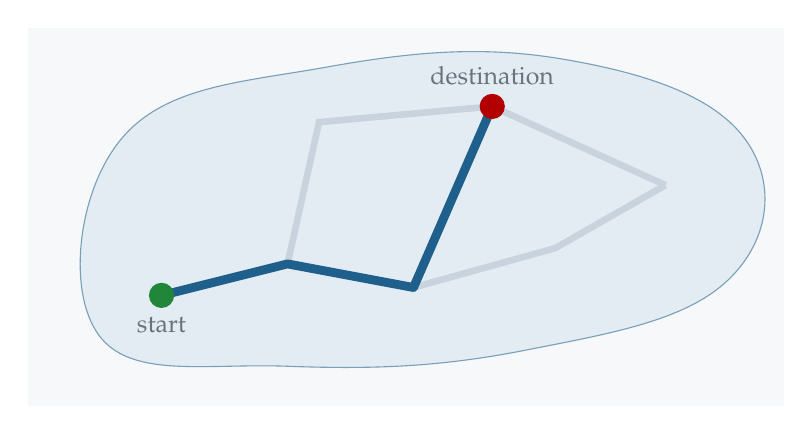
\begin{tikzpicture}[x=1cm,y=1cm]
  \fill[codebg] (-0.3,-0.4) rectangle (9.3,4.4);
  \fill[titlebg, draw=accent!60] plot[smooth cycle, tension=0.7] coordinates
    {(0.6,0.5) (3.0,0.1) (6.0,0.3) (8.6,1.2) (8.8,3.0) (6.5,4.0) (3.5,3.9) (0.9,3.0)};
  \draw[codeframe, line width=2.4pt] (1.4,1.0) -- (3.0,1.4) -- (4.6,1.1) -- (6.4,1.6) -- (7.8,2.4);
  \draw[codeframe, line width=2.4pt] (3.0,1.4) -- (3.4,3.2) -- (5.6,3.4);
  \draw[codeframe, line width=2.4pt] (4.6,1.1) -- (5.6,3.4) -- (7.8,2.4);
  \draw[accent, line width=3.2pt, line cap=round, line join=round]
    (1.4,1.0) -- (3.0,1.4) -- (4.6,1.1) -- (5.6,3.4);
  \fill[st] (1.4,1.0) circle (0.16);
  \fill[red!70!black] (5.6,3.4) circle (0.16);
  \node[font=\small, text=cm, anchor=north] at (1.4,0.85) {start};
  \node[font=\small, text=cm, anchor=south] at (5.6,3.55) {destination};
\end{tikzpicture}

\vfill
{\large A step-by-step tutorial\par}
\vspace{0.3cm}
{\normalsize Every line of code, every formula, nothing hidden\par}
\vspace{1.5cm}
\end{titlepage}

\frontmatter
\tableofcontents
\mainmatter

% ===========================================================================
\chapter{What we are going to build}

Kestrel Island is a small island in the North Atlantic, about four
kilometres across. It has a harbour town, Port Kestrel, a lake, two woods, a
brook, a lighthouse on its northern cape, and roads, lanes, tracks and
footpaths joining them all. It is also entirely imaginary: it exists only
as a file of numbers, \code{kestrel_island.map}.

By the end of this tutorial you will have written a program that turns that
file into a map in a window, and then lets you use it the way you use the
map app on a phone. Click where you want to start and where you want to go.
The program searches for the quickest way, and you can watch the search
spread out across the roads. Then a traveller sets off, a blue dot moving
along the highlighted route, while the program talks them through every
turn: ``In 300 m, turn left onto Mill Lane.''

\mappicture{nav_travel}

Press \code{x}, and the traveller takes a wrong turn on purpose. A moment
later the program notices that they have left the route, works out where
they are, and plans a new route from there, just as a satnav does.

There is a plain-text version too, for any two places:

\laterout{route.nex "beach car park" lighthouse}{route_beach}

\section{How digital maps work}

A map app looks like one program, but it is several quite different ideas
working together. Each of them is simple at heart, and this tutorial builds
every one of them in a few dozen lines of Nex.

\begin{description}[style=nextline, leftmargin=1.2em, itemsep=0.4em]
  \item[Positions on a round Earth.] A GPS gives positions as
    \emph{latitude} and \emph{longitude}: angles, not metres. We need to
    measure distances between them, which means a little spherical
    geometry (Chapter~\ref{ch:latlon}).
  \item[Flattening the Earth.] A screen is flat and the Earth is not.
    A \emph{map projection} turns latitude and longitude into flat
    $x$ and $y$ coordinates in metres. For a small island one simple
    projection is almost perfect (Chapter~\ref{ch:projection}).
  \item[Geometry.] Once things are flat, we need the distance from a point
    to a road, the area of a lake, whether a point is inside a wood, and
    which way a road points (Chapter~\ref{ch:geometry}).
  \item[The map as data.] The map file stores \emph{nodes} (single points)
    and lists of nodes that make roads and areas, the way OpenStreetMap,
    the world's largest open map, does it (Chapter~\ref{ch:mapfile}).
  \item[Drawing.] Turning that data into a picture people can read:
    colours, roads with outlines, labels that don't collide, a scale bar,
    and zooming in and out (Chapters~\ref{ch:drawing}
    and~\ref{ch:labels}).
  \item[Roads as a graph.] For finding a way, a map is a \emph{graph}:
    points joined by one-way or two-way connections, each with a length
    and a travel time (Chapter~\ref{ch:graph}).
  \item[Searching for a route.] Three classic algorithms: breadth-first
    search, Dijkstra's algorithm, and A*, which is what real route
    planners are built on (Chapters~\ref{ch:bfs}--\ref{ch:astar}).
  \item[Navigation.] Turning a route into instructions, following a
    moving traveller from noisy GPS fixes, and planning again when they go
    wrong (Chapters~\ref{ch:directions}--\ref{ch:wrongturn}).
\end{description}

Chapter~\ref{ch:livemap} puts it all together in the live map, and
Chapter~\ref{ch:next} looks at how the real thing differs: maps of whole
countries, tiles, traffic, and the clever tricks that answer a route
question about a continent in a few milliseconds.

\section{How this tutorial works}

We will build the whole project together, from an empty folder, in small
steps. Each step adds a few lines of code to one of the project's files,
and explains what the code does and why. When there is math behind the
code, we work through the math first, in simple steps, and then turn it
into code.

The code comes in boxes like this one. The title of the box says which
file the code belongs to, and where in the file it goes:

\begin{tcolorbox}[codebox, title={\textbf{New file}\enspace\texttt{example.nex}}]
\small Start a new file with this content.
\end{tcolorbox}
\begin{tcolorbox}[codebox, title={\texttt{example.nex}\enspace\textendash\enspace add at the end}]
\small Add this code at the end of the file.
\end{tcolorbox}
\begin{tcolorbox}[codebox, title={\texttt{example.nex}\enspace\textendash\enspace add before the line ...}]
\small Add this code at a particular place in the file, which the title tells you.
\end{tcolorbox}
\begin{tcolorbox}[codebox, title={\texttt{example.nex}\enspace\textendash\enspace continued}]
\small Add this code right after the code from the previous box.
\end{tcolorbox}

Green boxes are \emph{try-it} scripts: small throwaway programs that use
what we just built, so you can see it working. Their output follows in a
dark box, and when they draw a picture, the picture follows too:

\begin{tcolorbox}[trybox, title={\textbf{Try it}\enspace\texttt{try\_example.nex}}]
\small A small program to run now. It is not part of the project.
\end{tcolorbox}
\begin{tcolorbox}[outbox]
{\ttfamily\footnotesize\color{outfg}\$ nex try\_example.nex\\what it prints}
\end{tcolorbox}

Every program, every output and every picture in this tutorial was
produced by running the code exactly as printed here, so if your output
differs, compare your code with the boxes.

\section{What you need}

\begin{itemize}[nosep]
  \item \textbf{Nex}, installed so that the \code{nex} command works in a
        terminal. You should know the basics of the language: \code{let},
        functions and \code{result}, classes, loops, and contracts
        (\code{require}, \code{ensure}, \code{invariant}). We explain the
        less common features as we meet them.
  \item \textbf{The map file}, \code{kestrel_island.map}, from the
        \code{examples/digital_map} folder of the Nex distribution.
  \item \textbf{A display} for the live map in Chapter~\ref{ch:livemap}.
        Everything else, including all the pictures, works without one.
  \item \textbf{Math}: school geometry and trigonometry. We use
        Pythagoras' theorem, sine and cosine, and vectors (arrows), and we
        explain each one when it first comes up.
\end{itemize}

No mapping or graph library is used. Every distance, every projection,
every search and every pixel of the map is computed in Nex, in about 2,500
lines including comments and checks.

\section{The plan}

By the end you will have these files, each of which you will have written
yourself:

\begin{center}
\small
\begin{tabular}{@{}lll@{}}
\toprule
File & What it holds & Chapter \\
\midrule
\code{helpers.nex} & Printing numbers, distances and times neatly & \ref{ch:setup} \\
\code{geo.nex} & Latitude and longitude, flat points, the projection & \ref{ch:latlon}, \ref{ch:projection} \\
\code{geometry.nex} & Lines, segments, polygons and bearings & \ref{ch:geometry} \\
\code{island_map.nex} & Roads, areas and places, read from the map file & \ref{ch:mapfile} \\
\code{map_view.nex} & Drawing the map, at any zoom & \ref{ch:drawing}, \ref{ch:labels} \\
\code{road_graph.nex} & The roads as a graph, for driving or walking & \ref{ch:graph} \\
\code{search.nex} & Breadth-first search, Dijkstra's algorithm and A* & \ref{ch:bfs}--\ref{ch:astar} \\
\code{checks.nex} & Automatic checks of everything & \ref{ch:checks} \\
\code{directions.nex} & Turn-by-turn instructions & \ref{ch:directions} \\
\code{route.nex} & Directions between two places, printed & \ref{ch:directions} \\
\code{navigation.nex} & Following a traveller along a route & \ref{ch:following}, \ref{ch:wrongturn} \\
\code{simulation.nex} & A pretend traveller with a pretend GPS & \ref{ch:wrongturn} \\
\code{navigate.nex} & The live map & \ref{ch:livemap} \\
\bottomrule
\end{tabular}
\end{center}

% ===========================================================================
\chapter{Setting up}\label{ch:setup}

Make a folder for the project and go into it. Every file in this tutorial
goes in this one folder.

\begin{shell}
mkdir island
cd island
\end{shell}

Copy the map, \code{kestrel_island.map}, from the \code{examples/digital_map}
folder of the Nex distribution into it. It is a plain text file; we look
inside it in Chapter~\ref{ch:mapfile}.

\section{A first file: helpers}

The first file holds a few small helpers that the rest of the project uses
for printing.

First, a word about printing itself. Nex's \code{print} shows a string
with its quotes, as \code{"hello"}, which is handy when debugging but not
in a program's output. Every Nex program has a \code{Console} called
\code{console}, ready to use without creating it, and
\code{console.print_line("hello")} prints the text as it is, on a line of
its own. We use it for all our output.

Now numbers. Nex prints a \code{Real} with all its digits, like
\code{1879.3774630534463}, which is far more than anyone wants to read. The
built-in \code{format} writes a number with a fixed number of decimal
places, as text: \code{2.5.format(3)} is \code{"2.500"}, and
\code{(-3.14159).format(2)} is \code{"-3.14"}. It rounds to the nearest,
and a number exactly halfway rounds away from zero.

A navigator doesn't say ``in 347.2 metres''. It rounds, and the less
precise the better, as long as it is precise enough: ``in 350 m'',
``in 1.2 km''. Under a kilometre we round to the nearest 10 metres, which
is what \code{(metres / 10.0).round * 10} does; from a kilometre up we
give kilometres with one decimal. Times are given in whole minutes.

\begin{newfile}{helpers.nex}
-- helpers.nex: printing distances and times neatly, and finding the
-- user's files.

-- A distance the way a navigator says it: "40 m", "350 m", "1.2 km".
-- Under a kilometre it is rounded to 10 m, which is as precise as a
-- driver needs.
function distance_text(metres: Real): String
require
  non_negative: metres >= 0.0
do
  if metres < 995.0 then
    result := ((metres / 10.0).round * 10).to_string + " m"
  else
    result := (metres / 1000.0).format(1) + " km"
  end
end

-- A duration in whole minutes, "under a minute" or "1 h 05 min".
function duration_text(seconds: Real): String
require
  non_negative: seconds >= 0.0
do
  let minutes: Integer := (seconds / 60.0).round
  if minutes < 1 then
    result := "under a minute"
  elseif minutes < 60 then
    result := minutes.to_string + " min"
  else
    result := (minutes / 60).to_string + " h "
      + (minutes % 60).to_string.pad_start("0", 2) + " min"
  end
end
\end{newfile}

Why does \code{distance_text} switch to kilometres at 995 metres rather
than 1,000? Because 997 metres rounds to ``1000 m'', which looks odd; from
995 up we say ``1.0 km'' instead.

\code{minutes / 60} divides two \code{Integer}s, so it gives an
\code{Integer}, dropping the remainder: 65 minutes is 1 hour, and
\texttt{65~\%~60}, the remainder, is the 5 minutes left over. The minutes
always get two digits, \code{05} rather than \code{5}: the built-in
\code{pad_start} does that, as \code{s.pad_start("0", 2)} adds \code{"0"}s
on the left of \code{s} until it is 2 characters long.

The last helper finds a file the user names on the command line. The
\code{nex} launcher runs programs from its own installation folder, so a
plain name like \code{kestrel_island.map} would be looked for in the wrong
place. Every program also has \code{program}, the running
\code{Program}, which knows the folder you ran \code{nex} from:
\code{program.working_directory}. We put that in front of any name that
isn't already a full path:

\begin{append}{helpers.nex}
-- The full path of a file the user named. The `nex` launcher runs
-- programs from its own installation folder, so a relative name is
-- resolved against the folder the program was started from.
function user_path(raw: String): String do
  if raw.starts_with("/") then
    result := raw
  else
    result := program.working_directory + "/" + raw
  end
end
\end{append}

\section{Running a try-it script}

Let's check that it works. Make this file and run it:

\begin{tryit}{try_helpers.nex}
intern Helpers

console.print_line(2.5.format(3))
console.print_line((-3.14159).format(2))
console.print_line(distance_text(347.2) + ", " + distance_text(997.0) + ", "
  + distance_text(1234.0))
console.print_line(duration_text(25.0) + ", " + duration_text(150.0) + ", "
  + duration_text(3900.0))
\end{tryit}
\tryoutput{try_helpers}

\code{intern Helpers} finds \code{helpers.nex} in the same folder and loads
everything in it. The file does not need a class called \code{Helpers}:
ours holds only plain functions.

Try-it scripts are not part of the project. Keep them around to experiment
with, or delete them when you are done.

% ===========================================================================
\chapter{Where on Earth}\label{ch:latlon}

Every position on a digital map starts life as two numbers: a
\emph{latitude} and a \emph{longitude}. That is what a GPS receiver
reports, what the map file stores, and what you get if you ask a map app to
``share this location''. This chapter is about what those two numbers mean,
and how to measure the distance between two of them.

\section{Latitude and longitude}

Picture the Earth as a ball spinning about an axis through the North and
South Poles. The \emph{equator} is the circle around the middle, halfway
between the poles.

\begin{center}
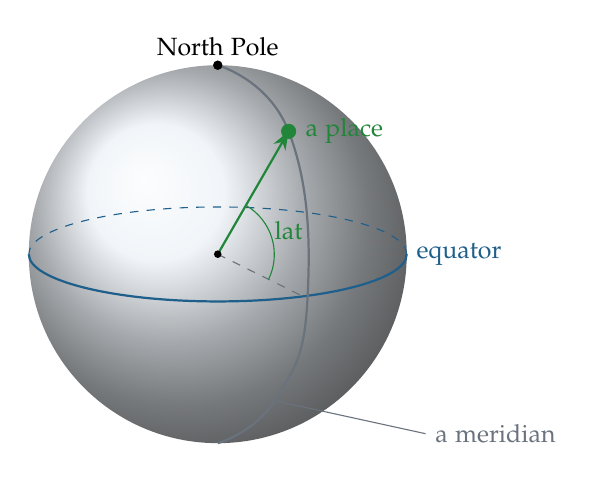
\begin{tikzpicture}[scale=1.2]
  \shade[ball color=titlebg!70!white] (0,0) circle (2);
  % the equator: the front half solid, the back half dashed
  \draw[accent, thick] (-2,0) arc[start angle=180, end angle=360, x radius=2, y radius=0.5];
  \draw[accent, dashed] (2,0) arc[start angle=0, end angle=180, x radius=2, y radius=0.5];
  % a meridian, from pole to pole across the front
  \draw[color=cm, thick] plot[smooth, tension=0.8] coordinates
    {(0,2) (0.75,1.3) (0.95,-0.47) (0.6,-1.55) (0,-2)};
  \coordinate (O) at (0,0);
  \coordinate (E) at (0.95,-0.47);
  \coordinate (P) at (0.75,1.3);
  \draw[color=cm, dashed] (O) -- (E);
  \draw[st, thick, -{Stealth}] (O) -- (P);
  \fill[st] (P) circle (0.08);
  \fill (O) circle (0.04);
  \draw[st] ($(O)!0.6cm!(E)$) arc[start angle=-26, end angle=60, radius=0.6cm];
  \node[st, font=\small] at (0.75,0.25) {lat};
  \fill (0,2) circle (0.05);
  \node[font=\small, above] at (0,2) {North Pole};
  \node[font=\small, right, st] at (P) {\ a place};
  \node[font=\small, text=accent, right] at (2,0) {equator};
  \draw[color=cm] (0.6,-1.55) -- (2.2,-1.9) node[right, font=\small, text=cm] {a meridian};
\end{tikzpicture}
\end{center}

\begin{itemize}
  \item \textbf{Latitude} says how far north or south a place is: the angle
    between the equator and the place, seen from the centre of the Earth.
    It runs from $0^\circ$ at the equator to $90^\circ$ at the North Pole,
    and to $-90^\circ$ at the South Pole. All the places with the same
    latitude form a circle around the Earth, called a \emph{parallel}.
  \item \textbf{Longitude} says how far east or west a place is. Every
    half circle from the North Pole to the South Pole is a
    \emph{meridian}, and longitude is the angle between a place's meridian
    and the one through Greenwich, in London, which was chosen in 1884 as
    the zero. It runs from $-180^\circ$ (west) to $180^\circ$ (east).
\end{itemize}

Kestrel Island's harbour is at latitude 47.052428 and longitude
-34.569106: about 47 degrees north of the equator, and about 34.6 degrees
west of Greenwich, out in the Atlantic. Positive latitudes are north,
negative ones south; positive longitudes are east, negative ones west.
People often write the same position as 47.05243\,N, 34.56911\,W.

Degrees with decimals are how computers store positions. Six decimal
places is plenty: one millionth of a degree of latitude is about 11
centimetres.

\section{The size of a degree}

How far is one degree? Going north along a meridian, a full circle of
$360^\circ$ is the whole way around the Earth, $2\pi R$, where $R$ is the
Earth's radius, about 6,371 km. So one degree of latitude is
\[
  \frac{2\pi \times 6\,371\,000}{360} \approx 111\,195 \text{ metres},
\]
everywhere on Earth.

A degree of longitude is different. The parallels get smaller towards the
poles, and a degree of longitude is $1/360$ of the parallel you are on. At
the equator that is 111 km too; at the poles it is nothing at all, because
every meridian meets there. We'll work out exactly how it shrinks in the
next chapter. What matters now is that a degree east and a degree north are
\emph{not} the same distance, so we can't find the distance between two
places by applying Pythagoras' theorem to their latitudes and longitudes.

\section{The distance between two places}

The shortest way between two places on a sphere is along a
\emph{great circle}: a circle around the sphere whose centre is the centre
of the sphere, such as the equator or any meridian. Airliners fly great
circles, which is why a flight from Europe to America goes up past
Greenland. The distance along it is given by the \emph{haversine formula}.

\begin{mathbox}[The haversine formula]
For two places with latitudes $\varphi_1, \varphi_2$ and longitudes
$\lambda_1, \lambda_2$, all in radians, work out
\[
  h = \sin^2\!\Big(\frac{\varphi_2 - \varphi_1}{2}\Big)
    + \cos\varphi_1 \cos\varphi_2 \, \sin^2\!\Big(\frac{\lambda_2 - \lambda_1}{2}\Big).
\]
Then the distance along the Earth's surface is
\[
  d = 2R \arcsin\sqrt{h}.
\]
\end{mathbox}

Where does that come from? Imagine a straight tunnel through the Earth
between the two places. Its length, the \emph{chord}, is easy to find with
3D coordinates: a place at latitude $\varphi$ and longitude $\lambda$ is at
\[
  R\,(\cos\varphi\cos\lambda,\ \cos\varphi\sin\lambda,\ \sin\varphi)
\]
measured from the centre of the Earth. Work out the squared distance
between two such points, simplify with a few trigonometric identities, and
you get $(2R)^2 h$, so the chord is $c = 2R\sqrt{h}$.

\begin{center}
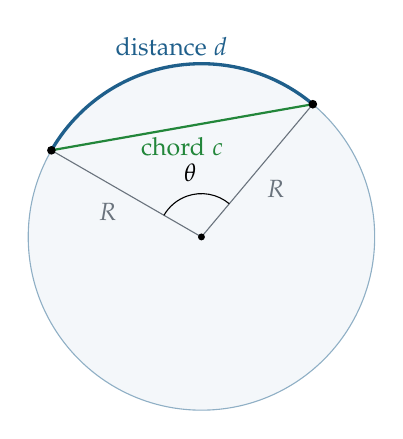
\begin{tikzpicture}[scale=1.1]
  \draw[accent!50, fill=titlebg!40] (0,0) circle (2);
  \coordinate (O) at (0,0);
  \coordinate (A) at (150:2);
  \coordinate (B) at (50:2);
  \draw[color=cm] (O) -- (A) node[midway, below left, font=\small] {$R$};
  \draw[color=cm] (O) -- (B) node[midway, below right, font=\small] {$R$};
  \draw[st, thick] (A) -- (B) node[midway, below, font=\small] {chord $c$};
  \draw[accent, very thick] (A) arc[start angle=150, end angle=50, radius=2]
    node[midway, above, font=\small] {distance $d$};
  \draw (O) ++(50:0.5) arc[start angle=50, end angle=150, radius=0.5];
  \node[font=\small] at (100:0.75) {$\theta$};
  \fill (A) circle (0.05) (B) circle (0.05) (O) circle (0.04);
\end{tikzpicture}
\end{center}

The chord and the two radii make a triangle with angle $\theta$ at the
centre. Cutting it in half gives two right-angled triangles, each with
hypotenuse $R$, angle $\theta/2$, and opposite side $c/2$, so
$c/2 = R\sin(\theta/2)$. Putting the two together,
$\sin(\theta/2) = c / 2R = \sqrt{h}$, so $\theta = 2\arcsin\sqrt{h}$, and
the distance along the surface, an arc of angle $\theta$ on a circle of
radius $R$, is $d = R\theta = 2R\arcsin\sqrt{h}$.

The name comes from old navigators' tables: $\sin^2(x/2)$ was called the
\emph{haversine} of $x$, ``half the versed sine''.

\section{Positions in Nex}

The Earth is not quite a sphere. It is about 21 km wider at the equator
than from pole to pole, and over long distances the haversine formula can
be out by up to half a percent. For an island a few kilometres across, a
sphere of the Earth's average radius is far more accurate than we need.

\begin{newfile}{geo.nex}
-- geo.nex: positions on the Earth, positions on a flat map, and the
-- projection that turns one into the other.

intern Helpers

class Earth
feature
  -- The Earth's mean radius in metres. The Earth is not quite a sphere
  -- (it is about 21 km wider at the equator than pole to pole), but for
  -- an island a few kilometres across a sphere is more than good enough.
  RADIUS = 6371000.0
end
\end{newfile}

A position is a pair of angles. The class checks that they are in range
when one is made, and \code{once} makes them unchangeable afterwards: a
position is a value, like a number, and code that wants a different
position makes a new one.

\begin{append}{geo.nex}
-- A position on the Earth's surface, in degrees, as a GPS reports it.
-- Latitude is north (+) or south (-) of the equator; longitude is east
-- (+) or west (-) of the meridian through Greenwich.
class Lat_Lon
create
  make(lat, lon: Real)
  require
    latitude_in_range: lat >= -90.0 and lat <= 90.0
    longitude_in_range: lon >= -180.0 and lon <= 180.0
  do
    latitude := lat
    longitude := lon
  end
feature
  once latitude: Real
  once longitude: Real
\end{append}

Now the haversine formula. Nex's trigonometry works in radians, so the
angles are converted first with \code{to_radians}.

\begin{continued}{geo.nex}
  -- The distance along the Earth's surface to `other`, in metres, by the
  -- haversine formula.
  distance_to(other: Lat_Lon): Real do
    let phi1: Real := latitude.to_radians
    let phi2: Real := other.latitude.to_radians
    let half_dphi: Real := (phi2 - phi1) / 2.0
    let half_dlambda: Real := (other.longitude - longitude).to_radians / 2.0
    -- In Nex, ^ binds as tightly as * and groups left to right, so
    -- a * b ^ 2 would mean (a * b) ^ 2. The parentheses matter.
    let h: Real := (half_dphi.sin ^ 2)
      + phi1.cos * phi2.cos * (half_dlambda.sin ^ 2)
    result := 2.0 * Earth.RADIUS * h.sqrt.min(1.0).asin
  ensure
    non_negative: result >= 0.0
  end
\end{continued}

Two details deserve a second look.

\textbf{The parentheses around the squares.} In mathematics, a power
binds more tightly than a multiplication, so $ab^2$ means $a(b^2)$. In
Nex, \code{^} has the same precedence as \code{*}, and operators of the
same precedence are worked out from left to right, so
\code{a * b ^ 2} means \code{(a * b) ^ 2}. Without the parentheses,
\code{phi1.cos * phi2.cos * half_dlambda.sin ^ 2} would square all three
factors, and every east-west distance would come out about 30\% too short
at Kestrel Island's latitude. It is the kind of mistake that runs without
complaint and gives plausible numbers, so it pays to remember.

\textbf{\code{h.sqrt.min(1.0)}.} In exact arithmetic $h$ is never more
than 1, but for two places on opposite sides of the Earth rounding can push
it a hair above, and $\arcsin$ of a number above 1 is undefined. Clamping
it costs nothing.

Last, a readable form for printing: the size of each angle, followed by its
direction.

\begin{continued}{geo.nex}
  -- "47.05123 N, 34.59877 W"
  to_string(): String do
    result := fixed(latitude.abs, 5) + when latitude >= 0.0 then " N, " else " S, " end
      + fixed(longitude.abs, 5) + when longitude >= 0.0 then " E" else " W" end
  end
end
\end{continued}

\begin{tryit}{try_geo.nex}
intern Geo

let harbour: Lat_Lon := create Lat_Lon.make(47.052428, -34.569106)
let lighthouse: Lat_Lon := create Lat_Lon.make(47.079318, -34.565277)
say("The harbour is at " + harbour.to_string())
say("The lighthouse is at " + lighthouse.to_string())
say("As the crow flies: " + fixed(harbour.distance_to(lighthouse), 1) + " m")

let london: Lat_Lon := create Lat_Lon.make(51.5074, -0.1278)
let new_york: Lat_Lon := create Lat_Lon.make(40.7128, -74.0060)
say("London to New York: " + fixed(london.distance_to(new_york) / 1000.0, 0) + " km")
\end{tryit}
\tryoutput{try_geo}

The lighthouse is about 3 km from the harbour. And London to New York
comes out at about 5,570 km, which is what an atlas says.

% ===========================================================================
\chapter{Flattening the Earth}\label{ch:projection}

A screen is flat. To draw a map we need every position as an $x$ and a $y$
on a flat surface, and it would be nice if those were in metres, so that
the ordinary geometry of the flat plane (Pythagoras' theorem, straight
lines, areas of polygons) just works. Turning latitude and longitude into
flat coordinates is called a \emph{map projection}.

\section{You can't flatten an orange peel}

Try to flatten a piece of orange peel and it tears or stretches. A sphere
cannot be laid flat without distorting it somehow, and every projection is
a choice about what to distort. Some keep areas right and bend shapes; some
keep shapes right in small patches and blow up areas far from the equator;
none keeps everything right everywhere.

\begin{aside}
\textbf{Web maps and Mercator.} Almost every map on the web, from
OpenStreetMap to the big commercial ones, uses the \emph{Web Mercator}
projection:
\[
  x = R\lambda, \qquad y = R \ln\tan\Big(\frac{\pi}{4} + \frac{\varphi}{2}\Big).
\]
Its great virtue is that it keeps angles right: a street corner that is a
right angle on the ground is a right angle on the screen, at every zoom.
Its great vice is scale: a metre on the ground is stretched by
$1/\cos\varphi$ on the map, more and more towards the poles. That is why
Greenland looks as big as Africa on a web map, when it is fourteen times
smaller. A map app that shows Mercator still has to measure distances on
the sphere, or correct for the stretch, as we do.
\end{aside}

The good news is that the smaller the area, the less any of this matters. A
piece of orange peel the size of a fingernail lies almost flat. Kestrel
Island is about four kilometres across, a fingernail on a twelve-thousand
kilometre ball, and the simplest projection there is will be accurate to a
few centimetres.

\section{How a degree of longitude shrinks}

The parallel at latitude $\varphi$ is a circle. Slice the Earth through
the poles and look at it side on:

\begin{center}
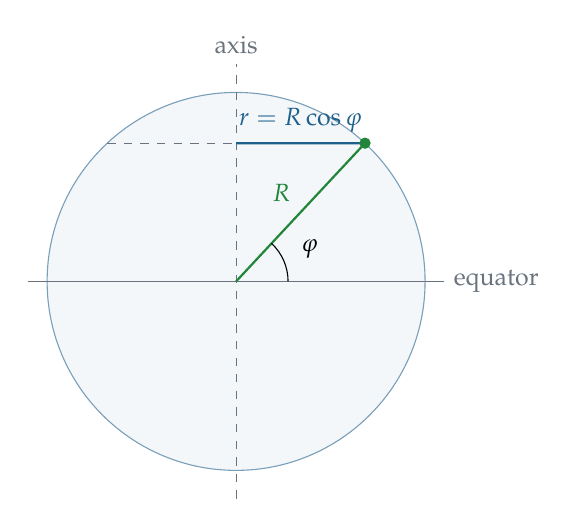
\begin{tikzpicture}[scale=1.2]
  \draw[accent!60, fill=titlebg!40] (0,0) circle (2);
  \draw[color=cm, dashed] (0,-2.3) -- (0,2.3) node[above, font=\small] {axis};
  \draw[color=cm] (-2.2,0) -- (2.2,0) node[right, font=\small] {equator};
  \coordinate (P) at (47:2);
  \draw[st, thick] (0,0) -- (P) node[midway, above left, font=\small] {$R$};
  \draw[accent, thick] (0,{2*sin(47)}) -- (P) node[midway, above, font=\small] {$r = R\cos\varphi$};
  \draw[color=cm, dashed] ({-2*cos(47)},{2*sin(47)}) -- (0,{2*sin(47)});
  \draw (0.55,0) arc[start angle=0, end angle=47, radius=0.55];
  \node[font=\small] at (24:0.85) {$\varphi$};
  \fill[st] (P) circle (0.06);
\end{tikzpicture}
\end{center}

The parallel's radius is the side of a right-angled triangle whose
hypotenuse is the Earth's radius $R$, with the angle $\varphi$ at the
centre, so it is $r = R\cos\varphi$. A degree of longitude is $1/360$ of
that circle, $2\pi R \cos\varphi / 360$: the 111,195 metres of a degree at
the equator, times $\cos\varphi$. At Kestrel Island's latitude,
$\cos 47^\circ \approx 0.68$, so a degree east is only about 75.8 km, while
a degree north is still 111.2 km.

\section{A local projection}

So here is the projection. Pick a centre for the map, at latitude
$\varphi_0$ and longitude $\lambda_0$. Then a place at $\varphi$, $\lambda$
(in degrees) goes to
\[
  x = (\lambda - \lambda_0) \cdot k_\lambda, \qquad
  y = (\varphi - \varphi_0) \cdot k_\varphi,
\]
where $k_\varphi = 2\pi R/360$ metres per degree of latitude, and
$k_\lambda = k_\varphi \cos\varphi_0$ metres per degree of longitude,
measured at the centre. The centre goes to $(0, 0)$; $x$ grows to the east
and $y$ to the north, both in metres. This is called the
\emph{equirectangular} projection.

It is exactly right along the centre's parallel, where we measured
$k_\lambda$. North or south of it, the true size of a degree of longitude
differs a little from $k_\lambda$. How little? Moving 1.6 km north, the
distance from the centre to Kestrel Island's northern tip, changes the
latitude by $0.0144^\circ$, which changes $\cos\varphi$ by about 0.03\%.
So an east-west distance up there comes out 0.03\% too long: 30
centimetres in a kilometre. For a road map, that is perfect.

Going back is just as easy: $\lambda = \lambda_0 + x / k_\lambda$ and
$\varphi = \varphi_0 + y / k_\varphi$.

\section{Points on the flat map}

A flat position is a \code{Point} with an \code{x} and a \code{y}. We will
use points in two ways: as positions, and as \emph{arrows} (vectors), such
as ``the arrow from the harbour to the lighthouse'', which is
\code{lighthouse - harbour}. Adding an arrow to a position moves the
position along the arrow; multiplying an arrow by a number stretches it.

Nex lets a class give a method the name of an arithmetic operator with
\code{alias}, so that \code{a + b} on two points means \code{a.plus(b)}.
That keeps geometry readable: \code{a + (b - a) * 0.5} is the point halfway
from \code{a} to \code{b}.

\begin{append}{geo.nex}
-- A position on a flat map, in metres: x east and y north of the map's
-- centre.
class Point
create
  make(px, py: Real) do
    x := px
    y := py
  end
feature
  once x: Real
  once y: Real

  plus(other: Point): Point alias "+" do
    result := create Point.make(x + other.x, y + other.y)
  end

  minus(other: Point): Point alias "-" do
    result := create Point.make(x - other.x, y - other.y)
  end

  -- This point scaled by k, as an arrow from the origin.
  times(k: Real): Point alias "*" do
    result := create Point.make(x * k, y * k)
  end
\end{append}

Two more operations on arrows. The \emph{length} of an arrow $(x, y)$ is
$\sqrt{x^2 + y^2}$, by Pythagoras; Nex's \code{hypot} computes exactly
that. The \emph{dot product} of two arrows, $a_x b_x + a_y b_y$, will be
useful in the next chapter, where we explain what it measures. The distance
between two points is the length of the arrow from one to the other.

\begin{continued}{geo.nex}
  -- The dot product, treating both points as arrows from the origin.
  dot(other: Point): Real do
    result := x * other.x + y * other.y
  end

  -- The length of this point as an arrow from the origin.
  length(): Real do
    result := x.hypot(y)
  end

  distance_to(other: Point): Real do
    result := (other - this).length
  ensure
    non_negative: result >= 0.0
  end

  -- "(123.4, -56.7)"
  to_string(): String do
    result := "(" + fixed(x, 1) + ", " + fixed(y, 1) + ")"
  end
end
\end{continued}

\section{The projection}

The projection holds the centre and the two scale factors, worked out once:

\begin{append}{geo.nex}
-- The local flat projection of the area around `centre`: a small piece of
-- the globe laid flat, with `centre` at (0, 0), x pointing east and y
-- north, both in metres.
--
-- A degree of latitude is the same length everywhere, but a degree of
-- longitude shrinks towards the poles, in proportion to the cosine of the
-- latitude: meridians meet at the poles. This projection measures both at
-- the centre's latitude. That is exact along the centre's parallel and
-- very nearly exact a few kilometres away, which is all a town or an
-- island needs. (A whole country or continent needs a cleverer projection.)
class Projection
create
  make(c: Lat_Lon) do
    centre := c
    metres_per_degree_lat := Earth.RADIUS * Real.PI / 180.0
    metres_per_degree_lon := metres_per_degree_lat * c.latitude.to_radians.cos
  end
feature
  centre: Lat_Lon
  metres_per_degree_lat: Real
  metres_per_degree_lon: Real

  to_point(p: Lat_Lon): Point do
    result := create Point.make(
      (p.longitude - centre.longitude) * metres_per_degree_lon,
      (p.latitude - centre.latitude) * metres_per_degree_lat)
  end

  to_lat_lon(p: Point): Lat_Lon do
    result := create Lat_Lon.make(
      centre.latitude + p.y / metres_per_degree_lat,
      centre.longitude + p.x / metres_per_degree_lon)
  ensure
    round_trip: to_point(result).distance_to(p) < 0.001
  end
invariant
  positive_scales: metres_per_degree_lat > 0.0 and metres_per_degree_lon > 0.0
end
\end{append}

The postcondition of \code{to_lat_lon} checks the two directions against
each other: projecting the answer forward again must land within a
millimetre of where we started. A contract like this is cheap insurance.
If someone later ``improves'' one direction and forgets the other, the
program stops at the first mismatch instead of drawing roads a few metres
off.

\begin{tryit}{try_projection.nex}
intern Geo

let harbour: Lat_Lon := create Lat_Lon.make(47.052428, -34.569106)
let lighthouse: Lat_Lon := create Lat_Lon.make(47.079318, -34.565277)
let flat: Projection := create Projection.make(create Lat_Lon.make(47.066, -34.5695))
let h: Point := flat.to_point(harbour)
let l: Point := flat.to_point(lighthouse)
say("harbour    " + h.to_string())
say("lighthouse " + l.to_string())
say("on the sphere:   " + fixed(harbour.distance_to(lighthouse), 2) + " m")
say("on the flat map: " + fixed(h.distance_to(l), 2) + " m")
say("back again: " + flat.to_lat_lon(l).to_string())

-- Pretending a degree is the same length both ways:
let k: Real := flat.metres_per_degree_lat
let naive: Point := create Point.make((lighthouse.longitude - harbour.longitude) * k,
  (lighthouse.latitude - harbour.latitude) * k)
say("degrees as if they were squares: " + fixed(naive.length(), 2) + " m")
\end{tryit}
\tryoutput{try_projection}

The flat map agrees with the sphere to within a few centimetres over three
kilometres. Pretending that a degree of longitude is as long as a degree of
latitude gets the distance wrong by several metres here, and it would be
much worse for two places side by side east and west. A map drawn that way
would look stretched sideways, by $1/\cos 47^\circ$, nearly one and a
half times.

% ===========================================================================
\chapter{A geometry toolkit}\label{ch:geometry}

With everything on a flat plane in metres, a map needs only a handful of
geometric tools, and they are all in this chapter:

\begin{itemize}[nosep]
  \item the length of a road, and the point a given distance along it;
  \item the point of a road closest to a GPS fix, and how far away it is;
  \item the area of a lake, and whether a point is inside a wood;
  \item which way a road points, and how sharply it turns.
\end{itemize}

\section{Lines}

On a map, a road or a river is a \emph{polyline}: a list of points joined
by straight \emph{segments}. Its length is the sum of the lengths of its
segments.

\begin{newfile}{geometry.nex}
-- geometry.nex: the flat geometry a map needs. Lines, segments and
-- polygons, and the directions of travel along them.

intern Geo

-- The total length of a line through `points`, in order.
function line_length(points: Array[Point]): Real do
  from
    let i: Integer := 1
  until
    i >= points.length
  do
    result := result + points.get(i - 1).distance_to(points.get(i))
    i := i + 1
  end
ensure
  non_negative: result >= 0.0
end
\end{newfile}

\code{result} starts at \code{0.0}, the zero value of \code{Real}, so the
loop can add to it straight away.

To find the point \code{d} metres along a line, walk along it segment by
segment, subtracting each segment's length from \code{d}, until \code{d}
is less than the length of the segment you are on. The point is then that
far into the segment: a fraction \code{d / length} of the way from its
start \code{a} to its end \code{b}, which is \code{a + (b - a) * (d / length)}.

\begin{append}{geometry.nex}
-- The point `d` metres along the line through `pts` (its last point if d
-- is past the end).
function point_along(pts: Array[Point], d: Real): Point
require
  not_empty: not pts.is_empty
do
  result := pts.get(pts.length - 1)
  let left: Real := d
  let found: Boolean := false
  from
    let i: Integer := 1
  until
    found or i >= pts.length
  do
    let a: Point := pts.get(i - 1)
    let b: Point := pts.get(i)
    let seg: Real := a.distance_to(b)
    if left <= seg and seg > 0.0 then
      result := a + (b - a) * (left / seg)
      found := true
    else
      left := left - seg
    end
    i := i + 1
  end
end

-- The average of some points: their centre of mass.
function average(pts: Array[Point]): Point
require
  not_empty: not pts.is_empty
do
  let sum: Point := create Point.make(0.0, 0.0)
  across pts as p do
    sum := sum + p
  end
  result := sum * (1.0 / pts.length.to_real)
end
\end{append}

The average of the corners of an area is a good enough place to write the
area's name on a map; we'll use it for exactly that.

\section{Segments, and the dot product}

When a GPS says you are at some point $p$, a navigator wants to know which
point of the road you are on: the point of the segment from $a$ to $b$
closest to $p$.

\begin{center}
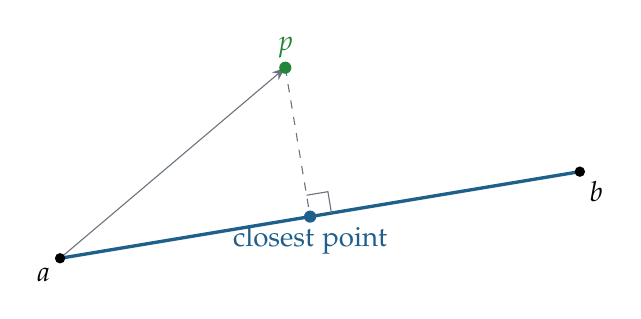
\begin{tikzpicture}[scale=1.1]
  \coordinate (A) at (0,0);
  \coordinate (B) at (6,1);
  \coordinate (P) at (2.6,2.2);
  \coordinate (C) at ($(A)!(P)!(B)$);
  \draw[accent, very thick] (A) -- (B);
  \draw[color=cm, dashed] (P) -- (C);
  \draw[color=cm, -{Stealth}] (A) -- (P);
  \fill (A) circle (0.06) node[below left] {$a$};
  \fill (B) circle (0.06) node[below right] {$b$};
  \fill[st] (P) circle (0.07) node[above] {$p$};
  \fill[accent] (C) circle (0.07) node[below] {closest point};
  \draw[color=cm] ($(C)!0.25cm!(B)$) -- ($($(C)!0.25cm!(B)$)!0.25cm!90:(B)$) -- ($(C)!0.25cm!(P)$);
\end{tikzpicture}
\end{center}

Every point of the segment is $a + t\,(b - a)$ for some $t$ from 0 (at $a$)
to 1 (at $b$). The closest one is where the dashed line from $p$ meets the
segment at a right angle, and the dot product finds it. For two arrows
$u$ and $v$,
\[
  u \cdot v = u_x v_x + u_y v_y = |u|\,|v|\cos\theta,
\]
where $\theta$ is the angle between them. So $u \cdot v / |v|$ is
$|u|\cos\theta$: how far $u$ reaches in the direction of $v$, the length of
its \emph{shadow} on $v$. With $u = p - a$ and $v = b - a$, the shadow is
how far along the segment the closest point is, and dividing by the
segment's length once more turns it into the fraction we want:
\[
  t = \frac{(p - a) \cdot (b - a)}{|b - a|^2}.
\]
If $t$ comes out below 0 or above 1, the right angle falls off the end of
the segment, and the nearest point is the nearer end. \code{clamp(0.0, 1.0)}
pulls $t$ back into range, which picks exactly that end.

\begin{append}{geometry.nex}
-- The point of the segment a-b closest to p.
--
-- Every point of the segment is a + t (b - a) for some t between 0 and 1.
-- The closest one to p is where the line from p meets the segment at a
-- right angle, which is at t = (p - a)·(b - a) / |b - a|^2. If that t is
-- below 0 or above 1, the right angle is off the end of the segment, and
-- the closest point is the nearer end.
function closest_point_on_segment(p, a, b: Point): Point do
  let ab: Point := b - a
  let len2: Real := ab.dot(ab)
  if len2 = 0.0 then
    result := a
  else
    let t: Real := ((p - a).dot(ab) / len2).clamp(0.0, 1.0)
    result := a + ab * t
  end
ensure
  no_further_than_ends: p.distance_to(result) <= p.distance_to(a) + 0.000001
    and p.distance_to(result) <= p.distance_to(b) + 0.000001
end

function distance_to_segment(p, a, b: Point): Real do
  result := p.distance_to(closest_point_on_segment(p, a, b))
end
\end{append}

The postcondition is a sanity check we can state without knowing anything
about dot products: the closest point can be no further away than either
end. The tiny allowance, a millionth of a metre, is for rounding.

\section{Polygons}

An area, such as a lake or a wood, is a \emph{polygon}: its outline is a
list of corners, and the last corner joins back to the first.

\subsection{Area: the shoelace formula}

The area of a polygon with corners $(x_0, y_0), \dots, (x_{n-1}, y_{n-1})$ is
\[
  A = \frac{1}{2}\,\Big|\sum_{i=0}^{n-1} (x_i\, y_{i+1} - x_{i+1}\, y_i)\Big|,
\]
where the corner after the last is the first again. It is called the
\emph{shoelace formula} because of the criss-cross pattern of the products
when the corners are written in a column.

Why does it work? Each term $x_i y_{i+1} - x_{i+1} y_i$ is twice the area
of the triangle from the origin to one edge of the outline, positive if
the edge goes anticlockwise around the origin and negative if it goes
clockwise. Going all the way round the outline, the triangles outside the
polygon are counted once each way and cancel, and what is left is the
polygon itself. The absolute value at the end makes the answer positive
whichever way round the corners are listed.

\begin{append}{geometry.nex}
-- The area inside a polygon, in square metres, by the shoelace formula.
-- `ring` lists the corners in order around the outline; the last corner
-- joins back to the first.
function polygon_area(ring: Array[Point]): Real
require
  is_polygon: ring.length >= 3
do
  let twice: Real := 0.0
  from
    let i: Integer := 0
  until
    i = ring.length
  do
    let p: Point := ring.get(i)
    let q: Point := ring.get((i + 1) % ring.length)
    twice := twice + (p.x * q.y - q.x * p.y)
    i := i + 1
  end
  result := twice.abs / 2.0
ensure
  non_negative: result >= 0.0
end
\end{append}

\texttt{(i + 1) \% ring.length} is the index of the next corner, which is
0 again after the last one.

\subsection{Inside or outside: casting a ray}

Is a point inside a polygon? Walk from the point in a straight line,
due east, all the way to the edge of the world, and count how many times
you cross the outline. Every crossing takes you from inside to outside or
back, and you end up outside. So if you crossed an odd number of times, you
started inside; an even number, outside.

\begin{center}
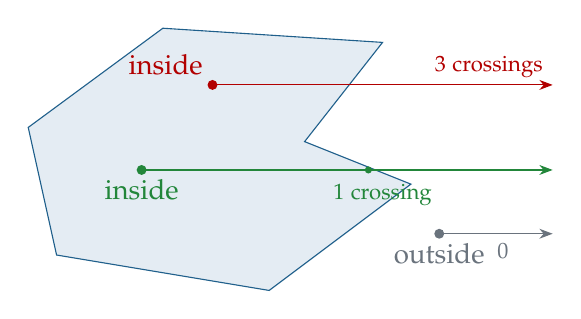
\begin{tikzpicture}[scale=0.9]
  \fill[titlebg, draw=accent] (0,0) -- (3,-0.5) -- (5,1) -- (3.5,1.6) -- (4.6,3)
    -- (1.5,3.2) -- (-0.4,1.8) -- cycle;
  \fill[st] (1.2,1.2) circle (0.07) node[below] {inside};
  \draw[st, -{Stealth}] (1.2,1.2) -- (7,1.2);
  \fill[st] (4.4,1.2) circle (0.05);
  \node[font=\footnotesize, st] at (4.6,0.85) {1 crossing};
  \fill[red!70!black] (2.2,2.4) circle (0.07) node[above left] {inside};
  \draw[red!70!black, -{Stealth}] (2.2,2.4) -- (7,2.4);
  \node[font=\footnotesize, text=red!70!black] at (6.1,2.65) {3 crossings};
  \fill[color=cm] (5.4,0.3) circle (0.07) node[below] {outside};
  \draw[color=cm, -{Stealth}] (5.4,0.3) -- (7,0.3);
  \node[font=\footnotesize, text=cm] at (6.3,0.05) {0};
\end{tikzpicture}
\end{center}

For each edge from $a$ to $b$, the ray crosses it if one end is above the
point and the other is not, and the edge passes the point's height to the
right of the point. Where along the edge does it pass that height? A
fraction $(p_y - a_y)/(b_y - a_y)$ of the way from $a$ to $b$, so at
$x = a_x + \frac{p_y - a_y}{b_y - a_y}(b_x - a_x)$.

\begin{append}{geometry.nex}
-- Whether p is inside the polygon, by casting a ray from p due east and
-- counting how many edges of the outline it crosses: an odd number means
-- inside, an even number outside.
function polygon_contains(ring: Array[Point], p: Point): Boolean
require
  is_polygon: ring.length >= 3
do
  let inside: Boolean := false
  from
    let i: Integer := 0
  until
    i = ring.length
  do
    let a: Point := ring.get(i)
    let b: Point := ring.get((i + 1) % ring.length)
    -- Does edge a-b cross the horizontal line through p, to p's right?
    if (a.y > p.y) /= (b.y > p.y) then
      let crossing_x: Real := a.x + (p.y - a.y) / (b.y - a.y) * (b.x - a.x)
      if crossing_x > p.x then
        inside := not inside
      end
    end
    i := i + 1
  end
  result := inside
end
\end{append}

The test \code{(a.y > p.y) /= (b.y > p.y)} compares two \code{Boolean}s:
it is true when exactly one end of the edge is above the point. It also
guarantees that \code{b.y - a.y} isn't zero, so the division is safe.

\section{Directions}

Navigators, compasses and sailors give directions as \emph{bearings}:
angles in degrees measured clockwise from north, so that north is
$0^\circ$, east $90^\circ$, south $180^\circ$ and west $270^\circ$.

Mathematicians measure angles the other way: anticlockwise from east (the
$x$ axis). The function $\operatorname{atan2}(y, x)$ gives that angle for
the arrow $(x, y)$, correctly in all four quarters of the circle. Swapping
its arguments swaps the roles of the two axes, which turns the
mathematicians' angle into the compass's: $\operatorname{atan2}(x, y)$
measures from north (the $y$ axis) clockwise towards east. In Nex,
\code{y.atan2(x)} is $\operatorname{atan2}(y, x)$, so the bearing of the
arrow $d$ is \code{d.x.atan2(d.y)}. It comes out between $-180^\circ$ and
$180^\circ$, and we add $360^\circ$ to the negative ones.

\begin{append}{geometry.nex}
-- The compass bearing from a to b, in degrees: 0 is north, 90 east, 180
-- south and 270 west, measured clockwise as on a compass.
function bearing(a, b: Point): Real do
  let d: Point := b - a
  result := d.x.atan2(d.y).to_degrees
  if result < 0.0 then
    result := result + 360.0
  end
ensure
  in_range: result >= 0.0 and result < 360.0
end

-- An arrow of length 1 pointing along a compass bearing.
function direction(heading: Real): Point do
  let r: Real := heading.to_radians
  result := create Point.make(r.sin, r.cos)
end
\end{append}

\code{direction} goes the other way, from a bearing back to an arrow. North
is $(0, 1)$ and east is $(1, 0)$, so the arrow is
$(\sin\theta, \cos\theta)$, again with sine and cosine in the opposite
places to the usual $(\cos\theta, \sin\theta)$.

When a traveller heading on bearing \code{before} turns onto a road with
bearing \code{after}, how far do they turn? The difference
\code{after - before}, but measured the short way round: heading
$350^\circ$ and turning to $10^\circ$ is a turn of $20^\circ$ to the
right, not $340^\circ$ to the left. So a difference over $180^\circ$ has
$360^\circ$ taken off, and one of $-180^\circ$ or less has $360^\circ$
added. Positive turns are to the right (clockwise), negative ones to the
left.

\begin{append}{geometry.nex}
-- How far a traveller turns when changing from heading `before` to
-- heading `after`: positive to the right, negative to the left, and never
-- more than half a turn either way.
function turn_angle(before, after: Real): Real do
  result := after - before
  if result > 180.0 then
    result := result - 360.0
  elseif result <= -180.0 then
    result := result + 360.0
  end
ensure
  in_range: result > -180.0 and result <= 180.0
end

-- The nearest of the eight compass points to a bearing: "north",
-- "north-east", ..., "north-west".
function compass_name(degrees: Real): String
require
  in_range: degrees >= 0.0 and degrees < 360.0
do
  let names: Array[String] := ["north", "north-east", "east", "south-east",
    "south", "south-west", "west", "north-west"]
  result := names.get(((degrees / 45.0).round) % 8)
end
\end{append}

The eight compass points are $45^\circ$ apart, so \code{degrees / 45.0},
rounded, is the number of the nearest one. A bearing of $350^\circ$ rounds
to 8, one past north-west, and \texttt{\% 8} turns that back into 0, north.

\begin{tryit}{try_geometry.nex}
intern Geometry

function pt(x, y: Real): Point do
  result := create Point.make(x, y)
end

let road: Array[Point] := [pt(0.0, 0.0), pt(300.0, 0.0), pt(300.0, 400.0)]
console.print_line("the road is " + fixed(line_length(road), 0) + " m long")
console.print_line("200 m along it: " + point_along(road, 200.0).to_string())
console.print_line("500 m along it: " + point_along(road, 500.0).to_string())
let fix: Point := pt(120.0, 9.0)
console.print_line("closest point to " + fix.to_string() + ": "
  + closest_point_on_segment(fix, road.get(0), road.get(1)).to_string()
  + ", " + fixed(distance_to_segment(fix, road.get(0), road.get(1)), 1) + " m away")

let field: Array[Point] := [pt(0.0, 0.0), pt(100.0, 0.0), pt(100.0, 50.0), pt(0.0, 50.0)]
console.print_line("the field is " + fixed(polygon_area(field), 0) + " square metres")
console.print_line("(50, 25) inside? " + polygon_contains(field, pt(50.0, 25.0)).to_string)
console.print_line("(150, 25) inside? " + polygon_contains(field, pt(150.0, 25.0)).to_string)

let heading: Real := bearing(road.get(0), road.get(1))
let turned: Real := bearing(road.get(1), road.get(2))
console.print_line("first heading " + fixed(heading, 0) + " (" + compass_name(heading) + "), then "
  + fixed(turned, 0) + " (" + compass_name(turned) + ")")
console.print_line("the turn: " + fixed(turn_angle(heading, turned), 0) + " degrees")
\end{tryit}
\tryoutput{try_geometry}

The road heads east, then turns north: a turn of $-90^\circ$, a left turn.
\code{to_string} without parentheses is how Nex writes a call with no
arguments on a built-in value; \code{to_string()} works too.

% ===========================================================================
\chapter{The map as data}\label{ch:mapfile}

A digital map is not a picture. It is a database of things (roads,
rivers, lakes, buildings, places) with their positions, and the pictures
are drawn from that database whenever they are needed, at whatever zoom
and in whatever style. That is how one map can be drawn for a car's
dashboard and for a hiker's phone, and why the same data can answer
``how do I get there?''.

\section{Nodes and ways}

OpenStreetMap, the free map of the world that anyone can edit, stores its
whole database with just three kinds of element:
\begin{itemize}[nosep]
  \item a \textbf{node} is a single point, with a latitude and a longitude;
  \item a \textbf{way} is an ordered list of nodes: a road, a river, or,
    if its last node is its first, the outline of an area;
  \item a \textbf{relation} groups other elements, such as all the roads
    of a bus route.
\end{itemize}
Every element also carries \emph{tags} that say what it is, such as
\code{highway=residential} or \code{name=Mill Lane}.

Our map file is a small cousin of that design. Here is the start of it:

\begin{shell}
# Kestrel Island: an imaginary island in the North Atlantic.
# ...
map Kestrel Island

node 1 47.053148 -34.574915
node 2 47.053148 -34.573595
node 3 47.053148 -34.572275
...
road street two-way Quay Street: 1 2 3 4 5 6 7 8 9
road street one-way Market Street: 10 11 12 13 14 15 16 17 18
...
road main two-way Coast Road: 48 49 50 51 52 53 54 55 56 ...
road path two-way Lake Walk: 100 144 145 146 147 148 149 ...
...
area land Kestrel Island: 174 175 176 177 178 179 180 ...
area water Mirror Lake: 238 239 240 241 242 243 244 245 ...
river Kestrel Brook: 256 257 258 259 260 261 262 263 264 265
...
place The Harbour: 266
place Lighthouse: 271
\end{shell}

Each line is one record. A \code{node} line gives a node's id and its
position. A \code{road} line gives the road's kind (\code{main},
\code{lane}, \code{street}, \code{track} or \code{path}), whether it is
one-way, its name, and then, after the colon, its nodes in order. An
\code{area} line gives the kind of area (\code{land}, \code{water},
\code{wood}, \code{sand} or \code{town}), its name, and the nodes around its
outline. A \code{river} is a line of nodes, from its source to the sea. A
\code{place} is a name for a single node.

Keeping the positions in nodes, and having everything else refer to nodes
by id, has a lovely consequence: \emph{roads that share a node are
joined}. Node 1 is the first node of both Quay Street and Anchor Street,
so that corner is a junction, and anyone on Quay Street can turn into
Anchor Street there. Two roads that merely cross on the map without
sharing a node, such as a road on a bridge over another, are not joined.
The connections that route planning needs are all in the data, without any
geometry.

The order of a one-way road's nodes matters too: Market Street may be
driven only from node 10 towards node 18, which on the map is from west to
east.

\section{Kinds of road}

A road's kind decides how it is drawn and how fast you can travel on it. A
fixed set of named values like this is what an \emph{enumeration} is for.
In Nex, an \code{enum union} declares one: the values are
\code{Road_Kind.Main}, \code{Road_Kind.Lane} and so on, each of them a
single shared object, and \code{Road_Kind.values} is an array of them all,
in the order they are written.

\begin{newfile}{island_map.nex}
-- island_map.nex: the map itself. Nodes, roads, areas, a river and named
-- places, read from a .map file.

intern Geo
intern Geometry
intern io/Path

-- The kinds of road, from fastest to slowest. A footpath is for walkers
-- only.
enum union Road_Kind
  Main
  Lane
  Street
  Track
  Footpath
end

-- The kind written in a .map file: "main", "lane", "street", "track" or
-- "path".
function road_kind(word: String): Road_Kind do
  if word = "main" then
    result := Road_Kind.Main
  elseif word = "lane" then
    result := Road_Kind.Lane
  elseif word = "street" then
    result := Road_Kind.Street
  elseif word = "track" then
    result := Road_Kind.Track
  elseif word = "path" then
    result := Road_Kind.Footpath
  else
    raise "unknown road kind: " + word
  end
end
\end{newfile}

The file says \code{path}, but the value is called \code{Footpath}, because
\code{Path} is already the name of the library class for file paths, which
we use below to read the file.

The \code{raise} at the end matters. \code{Road_Kind} is not an optional
type, so the function must return one on every path, and there is no
sensible kind for a word we don't know. Raising an error is the honest
answer, and Nex accepts it, since a path that raises never returns.

\section{Roads, areas, rivers and places}

Each kind of record becomes a small class. They hold node \emph{ids}, not
positions, exactly as the file does.

\begin{append}{island_map.nex}
-- A road: a line through two or more nodes, in order.
class Road
create
  make(road_name: String, road_kind: Road_Kind, one_way: Boolean, ids: Array[Integer])
  require
    at_least_two_nodes: ids.length >= 2
  do
    name := road_name
    kind := road_kind
    is_one_way := one_way
    node_ids := ids
  end
feature
  once name: String
  once kind: Road_Kind
  -- A one-way road may be driven only from its first node towards its last.
  once is_one_way: Boolean
  once node_ids: Array[Integer]
invariant
  at_least_two_nodes: node_ids.length >= 2
end

-- An area: the polygon through its nodes, the last joined back to the
-- first. The kind is "land", "water", "wood", "sand" or "town".
class Area
create
  make(area_kind, area_name: String, ids: Array[Integer])
  require
    at_least_three_nodes: ids.length >= 3
  do
    kind := area_kind
    name := area_name
    node_ids := ids
  end
feature
  once kind: String
  once name: String
  once node_ids: Array[Integer]
invariant
  at_least_three_nodes: node_ids.length >= 3
end

-- A river, as a line through its nodes from source to sea.
class River
create
  make(river_name: String, ids: Array[Integer])
  require
    at_least_two_nodes: ids.length >= 2
  do
    name := river_name
    node_ids := ids
  end
feature
  once name: String
  once node_ids: Array[Integer]
end

-- A named place: a single node with a name.
class Place
create
  make(place_name: String, id: Integer) do
    name := place_name
    node_id := id
  end
feature
  once name: String
  once node_id: Integer
end
\end{append}

A road needs at least two nodes and an area at least three, so the
constructors require it. A road with one node, or a lake with two corners,
would be a mistake in the map file, and it is far better to stop when the
file is read than to crash much later while drawing.

\section{Reading the file}

The map itself keeps every node's position twice: as latitude and longitude
from the file, and as a flat point in metres, for everything else. Both are
\code{Map}s from node ids. It reads the file line by line, skipping blank
lines and comments.

\begin{append}{island_map.nex}
class Island_Map
create
  -- Read a map from a .map file (see kestrel_island.map for the format).
  load(file: String) do
    name := "Untitled"
    positions := {}
    points := {}
    roads := []
    areas := []
    rivers := []
    places := []
    let line_number: Integer := 0
    across create Path.make(file).read_text().split("\n") as raw do
      line_number := line_number + 1
      let line: String := raw.trim()
      if line /= "" and not line.starts_with("#") then
        do
          read_line(line)
        rescue
          raise file + ", line " + line_number.to_string + ": " + exception.to_string
        end
      end
    end
    if positions.is_empty then
      raise file + ": no nodes"
    end
    projection := create Projection.make(middle_of(positions.values))
    across positions as entry do
      points.put(entry.key, projection.to_point(entry.value))
    end
  end
\end{append}

Two things happen after the reading.

First, the projection. Its centre is the middle of the map: halfway
between the most northern and most southern nodes, and halfway between
the most eastern and most western. That keeps every node within a couple
of kilometres of the centre, where the projection is most accurate.

Second, every position is projected once, and the flat points stored by
node id. From here on, nothing else in the project needs to know that the
Earth is round.

If anything goes wrong reading a line, the \code{rescue} catches the
error, and raises it again with the file name and line number in front, so
that a mistake in a 300-line file can be found at once.

Now the queries, starting with positions:

\begin{continued}{island_map.nex}
feature
  name: String
  -- Every node's position on the globe, by node id...
  positions: Map[Integer, Lat_Lon]
  -- ...and on the flat map, in metres from the map's centre.
  points: Map[Integer, Point]
  projection: Projection
  roads: Array[Road]
  areas: Array[Area]
  rivers: Array[River]
  places: Array[Place]

  -- The flat position of a node.
  point(id: Integer): Point
  require
    known_node: points.contains_key(id)
  do
    result := points.get(id)
  end

  -- The flat positions of several nodes, in order.
  points_of(ids: Array[Integer]): Array[Point] do
    across ids as id do
      result.add(point(id))
    end
  ensure
    same_length: result.length = ids.length
  end

  -- The smallest and largest x and y of all the nodes.
  min_x(): Real do
    result := extreme(true, true)
  end

  max_x(): Real do
    result := extreme(true, false)
  end

  min_y(): Real do
    result := extreme(false, true)
  end

  max_y(): Real do
    result := extreme(false, false)
  end
\end{continued}

\code{points_of} adds to \code{result} straight away: a routine returning
an \code{Array} starts with a fresh empty one.

People name places loosely, so \code{find_place} accepts any part of a
name, ignoring capitals: \code{"mill"} finds Old Mill. An exact match is
looked for first, so that a name that happens to be part of another
(Long Sands inside ``Long Sands Car Park'', say) can still be chosen.

Then a question every map app answers: what is at this point? Areas can
overlap (the lake lies inside the island), and the file lists the ones
drawn on top later, so the answer is the last area in the list that
contains the point. The \code{?Place} and \code{?Area} return types say
that the answer may be \code{nil}: no such place, or out at sea.

\begin{continued}{island_map.nex}
  -- The place called `query`, ignoring case; failing that, the first
  -- place whose name contains it ("mill" finds "Old Mill").
  find_place(query: String): ?Place do
    let wanted: String := query.to_lower()
    across places as p do
      if result = nil and p.name.to_lower() = wanted then
        result := p
      end
    end
    across places as p do
      if result = nil and p.name.to_lower().contains(wanted) then
        result := p
      end
    end
  end

  -- The area at a point, or nil out at sea. Areas listed later are drawn
  -- on top of earlier ones (the lake on top of the island), so the last
  -- one that contains the point is the one you would see there.
  area_at(p: Point): ?Area do
    across areas as a do
      if polygon_contains(points_of(a.node_ids), p) then
        result := a
      end
    end
  end
\end{continued}

Last, the private routines that do the reading. A line is split at its
colon into a \emph{head}, the words before it, and the node ids after it.
Every id must already have appeared in a \code{node} line; otherwise the
file is broken, and we say so. Then the first word says what kind of
record the line is.

\begin{continued}{island_map.nex}
private feature
  read_line(line: String) do
    let colon: Integer := line.index_of(":")
    let head: Array[String] := []
    let ids: Array[Integer] := []
    if colon >= 0 then
      head := words(line.substring(0, colon))
      across words(line.substring(colon + 1, line.length)) as w do
        let id: Integer := w.to_integer
        if not positions.contains_key(id) then
          raise "node " + w + " is used before it is defined"
        end
        ids.add(id)
      end
    else
      head := words(line)
    end
    let record: String := head.get(0)
    if record = "map" then
      name := joined(head, 1)
    elseif record = "node" then
      positions.put(head.get(1).to_integer,
        create Lat_Lon.make(head.get(2).to_real, head.get(3).to_real))
    elseif record = "road" then
      roads.add(create Road.make(joined(head, 3), road_kind(head.get(1)),
        head.get(2) = "one-way", ids))
    elseif record = "area" then
      areas.add(create Area.make(head.get(1), joined(head, 2), ids))
    elseif record = "river" then
      rivers.add(create River.make(joined(head, 1), ids))
    elseif record = "place" then
      places.add(create Place.make(joined(head, 1), ids.get(0)))
    else
      raise "unknown record: " + record
    end
  end

  -- The words of s, however many spaces separate them.
  words(s: String): Array[String] do
    across s.split(" ") as w do
      if w /= "" then
        result.add(w)
      end
    end
  end

  -- The words from index `first` on, joined back with single spaces.
  joined(ws: Array[String], first: Integer): String do
    result := " ".join(ws.drop(first))
  end
\end{continued}

A name can have spaces in it, so it is everything in the head after the
fixed words: \code{joined(head, 3)} on
\code{road street one-way Market Street} is \code{Market Street}.

Finally, the middle of a list of positions, for the projection's centre,
and the extremes of the flat points, for fitting the map on a screen:

\begin{continued}{island_map.nex}
  -- The point halfway between the most northern and southern latitudes,
  -- and the most eastern and western longitudes.
  middle_of(all: Array[Lat_Lon]): Lat_Lon do
    let south: Real := 90.0
    let north: Real := -90.0
    let west: Real := 180.0
    let east: Real := -180.0
    across all as p do
      south := south.min(p.latitude)
      north := north.max(p.latitude)
      west := west.min(p.longitude)
      east := east.max(p.longitude)
    end
    result := create Lat_Lon.make((south + north) / 2.0, (west + east) / 2.0)
  end

  -- The smallest (or largest) x (or y) of all the nodes.
  extreme(along_x, smallest: Boolean): Real do
    let first: Boolean := true
    across points.values as p do
      let v: Real := when along_x then p.x else p.y end
      if first or (smallest and v < result) or (not smallest and v > result) then
        result := v
        first := false
      end
    end
  end
end
\end{continued}

\section{Exploring the island}

Now we can load the island and ask it questions. One hectare is
10,000 square metres, about the size of a football pitch and a half.

\begin{tryit}{try_island.nex}
intern Island_Map
intern Helpers

let island: Island_Map := create Island_Map.load(user_path("kestrel_island.map"))
console.print_line(island.name + ": " + island.positions.size.to_string + " nodes, "
  + island.roads.length.to_string + " roads, " + island.places.length.to_string + " places")
console.print_line("centred on " + island.projection.centre.to_string())
console.print_line((island.max_x() - island.min_x()).format(0) + " m from west to east, "
  + (island.max_y() - island.min_y()).format(0) + " m from south to north")
console.print_line("")
across island.areas as a do
  console.print_line(a.name.pad_end(" ", 16) + (polygon_area(island.points_of(a.node_ids)) / 10000.0).format(1)
    .pad_start(" ", 7) + " hectares of " + a.kind)
end
console.print_line("")
across Road_Kind.values as kind do
  let total: Real := 0.0
  across island.roads as r do
    if r.kind = kind then
      total := total + line_length(island.points_of(r.node_ids))
    end
  end
  console.print_line(kind.to_string.pad_end(" ", 10) + distance_text(total).pad_start(" ", 7))
end
console.print_line("")
across island.places as p do
  if ?island.area_at(island.point(p.node_id)) as a then
    console.print_line(p.name + when a.kind = "land" then " is on " else " is in " end + a.name)
  end
end
\end{tryit}
\tryoutput{try_island}

The island is about ten square kilometres, and the program agrees with the
map: Kestrel Peak is in Hollow Wood, and the school and the market are in
Port Kestrel.

What happens if the file has a mistake in it? This script writes a small
broken map and tries to load it:

\begin{tryit}{try_bad_map.nex}
intern Island_Map
intern Helpers

let file: String := user_path("broken.map")
create Path.make(file).write_text("map Broken\nnode 1 47.0 -34.0\nnode 2 47.0 -34.1\nroad lane two-way Short Lane: 1 2 3\n")
do
  let island: Island_Map := create Island_Map.load(file)
rescue
  console.print_line(exception.to_string.replace(user_path(""), ""))
end
\end{tryit}
\tryoutput{try_bad_map}

The error names the file, the line and the problem: Short Lane uses a node
that the file never defines.

% ===========================================================================
\chapter{Drawing the map}\label{ch:drawing}

Now for a picture. Nex's \code{graphics/Canvas} library gives us a canvas
of pixels to draw on, which we can save as a PNG file or show in a window.
This chapter draws the island's land, water, woods and roads; the next one
adds the words.

\section{From metres to pixels}

The canvas does the arithmetic of turning map coordinates into pixels for
us. We tell it which rectangle of the map to show, with
\code{set_x_scale(x0, x1)} and \code{set_y_scale(y0, y1)}, and then draw
in map coordinates: metres. A canvas \code{w} pixels wide showing $x$ from
$x_0$ to $x_1$ puts the point $x$ at pixel column
\[
  \frac{x - x_0}{x_1 - x_0}\, w,
\]
and similarly for $y$, except that pixel rows count \emph{down} from the
top of the image, while our $y$ counts \emph{up} towards the north. The
canvas turns it over for us, so north is at the top, as on any map.

The one thing we must get right is the shape. If the rectangle we show
has a different shape from the canvas, the map is stretched. So instead of
choosing a rectangle, we choose a \emph{centre} and a \emph{scale}, in
metres per pixel, and work out the rectangle from those:
\[
  x_0 = c_x - \tfrac{1}{2}\, w \cdot \text{scale}, \qquad
  x_1 = c_x + \tfrac{1}{2}\, w \cdot \text{scale},
\]
and the same for $y$ with the canvas's height. Every pixel is then the same
number of metres wide as it is high. Zooming in is making the scale
smaller; panning is moving the centre.

There is one complication, for later. In Chapter~\ref{ch:livemap} the live
map draws panels across the top and the bottom of the window, with
instructions and settings, and the map should be centred in the space
between them. So the view knows how many pixels at the top and bottom are
covered, its \emph{insets}, and centres the map in the rest. For now both
are zero.

\section{The colours}

Map makers spend a long time on colours. Ours are close to the ones
OpenStreetMap's standard style uses, which are tuned so that the important
things (roads and names) stand out from the background (land and water):
pale, quiet colours for areas, stronger ones for roads.

\begin{newfile}{map_view.nex}
-- map_view.nex: drawing the map on a canvas, at any zoom.

intern Island_Map
intern Helpers
intern graphics/Canvas

-- The map's colours.
class Palette
feature
  SEA = create Color.make(170, 211, 223)
  LAND = create Color.make(242, 239, 233)
  SAND = create Color.make(240, 228, 190)
  TOWN = create Color.make(232, 224, 218)
  WOOD = create Color.make(181, 214, 160)
  WATER = create Color.make(170, 211, 223)
  RIVER = create Color.make(120, 175, 205)
  CASING = create Color.make(150, 140, 130)
  MAIN_ROAD = create Color.make(250, 205, 140)
  MAIN_CASING = create Color.make(205, 140, 70)
  MINOR_ROAD = create Color.make(255, 255, 255)
  TRACK = create Color.make(160, 115, 70)
  FOOTPATH = create Color.make(225, 95, 80)
  LABEL = create Color.make(60, 60, 60)
  ROAD_LABEL = create Color.make(90, 85, 80)
  WATER_LABEL = create Color.make(50, 110, 150)
  HALO = create Color.make_rgba(255, 255, 255, 220)
end
\end{newfile}

\code{HALO} is white and slightly see-through: its fourth number, the
\emph{alpha}, is 220 out of 255.

\section{The view}

A \code{Map_View} holds the map, a canvas, and where the canvas is looking.

\begin{append}{map_view.nex}
class Map_View
create
  -- A view of `m` on a new canvas `width` by `height` pixels, showing the
  -- whole map.
  make(m: Island_Map, width, height: Integer) do
    island := m
    canvas := create Canvas.make(width, height)
    centre := create Point.make(0.0, 0.0)
    metres_per_pixel := 1.0
    show_all()
  end
feature
  island: Island_Map
  canvas: Canvas
  -- The point of the map at the middle of the canvas...
  centre: Point
  -- ...and how many metres of the map one pixel covers. Bigger means
  -- zoomed out.
  metres_per_pixel: Real

  -- Pixels at the top and bottom of the canvas that something else covers
  -- (a program's own panels), to keep the scale bar and north arrow clear
  -- of.
  inset_top: Real
  inset_bottom: Real

  set_insets(top, bottom: Real)
  require
    non_negative: top >= 0.0 and bottom >= 0.0
    room_left: top + bottom < canvas.height.to_real
  do
    inset_top := top
    inset_bottom := bottom
    look_at(centre, metres_per_pixel)
  end
\end{append}

To show the whole map, take the map's width and height in metres, and see
how many metres per pixel it takes to fit each of them on the canvas. The
larger of the two fits both; making it 8\% larger leaves a margin of sea
all round.

\begin{continued}{map_view.nex}
  -- Zoom and pan so that the whole map fits, with a little sea around it.
  show_all() do
    let w: Real := island.max_x() - island.min_x()
    let h: Real := island.max_y() - island.min_y()
    let mpp: Real := (w / canvas.width.to_real).max(h / free_height()) * 1.08
    look_at(create Point.make((island.min_x() + island.max_x()) / 2.0,
      (island.min_y() + island.max_y()) / 2.0), mpp)
  end

  -- Centre the view on c, at mpp metres per pixel. "Centre" means the
  -- middle of the part of the canvas that the insets leave free.
  look_at(c: Point, mpp: Real)
  require
    positive_scale: mpp > 0.0
  do
    centre := c
    metres_per_pixel := mpp
    let half_w: Real := canvas.width.to_real * mpp / 2.0
    let top: Real := c.y + (inset_top + free_height() / 2.0) * mpp
    canvas.set_x_scale(c.x - half_w, c.x + half_w)
    canvas.set_y_scale(top - canvas.height.to_real * mpp, top)
  end

  -- The height of the canvas that the insets leave free, in pixels.
  free_height(): Real do
    result := canvas.height.to_real - inset_top - inset_bottom
  end

  -- A distance on the canvas in pixels, as metres on the map.
  metres(pixels: Real): Real do
    result := pixels * metres_per_pixel
  end
\end{continued}

In \code{look_at}, the centre \code{c} should land in the middle of the
free part of the canvas: \code{inset_top + free_height() / 2.0} pixels
down from the top. So the top edge of the canvas is that many pixels'
worth of metres north of \code{c}, and the bottom edge is the canvas's
whole height further south.

\code{metres} converts a size in pixels into metres at the current scale.
We use it for everything that should look the same size at every zoom:
dots, arrows, the gap between a label and its place. Roads, too, are drawn
a fixed number of pixels wide, however far we zoom, as on every map app.

\section{Layers}

A map is drawn in \emph{layers}, from the bottom up: the sea first, then
the land on top of it, then lakes and woods on the land, then rivers, then
roads, then the dots for places. Each layer paints over the ones below.

\begin{continued}{map_view.nex}
  -- Draw the whole map, layer by layer, from the sea up.
  draw_map() do
    canvas.clear(Palette.SEA)
    draw_areas()
    draw_rivers()
    draw_roads()
    draw_places()
    draw_scale_bar()
    draw_north_arrow()
  end

  draw_areas() do
    across island.areas as a do
      canvas.set_pen_color(area_color(a.kind))
      fill_polygon(island.points_of(a.node_ids))
    end
  end

  draw_rivers() do
    across island.rivers as r do
      line(island.points_of(r.node_ids), Palette.RIVER, 2.5)
    end
  end
\end{continued}

The order of the areas in the map file is the order they are drawn: the
island first, then the town, the woods and the lake on top of it. That is
why \code{area_at} in the last chapter took the \emph{last} area containing
a point.

\section{Roads}

Look closely at a road on a printed map or a map app. It is not one line
but two: a darker, wider line underneath, called the \emph{casing}, and
the road's own colour on top. The casing gives the road an outline, which
makes it stand out from the land. And because every road's casing is drawn
before any road's colour, where two roads meet the colour of one paints
over the casing of the other, and the junction looks joined, not crossed.

\begin{center}

\begin{tikzpicture}[x=1cm,y=1cm]
  \begin{scope}
    \draw[line width=7pt, black!45] (0,0) -- (3,0);
    \draw[line width=5pt, white] (0,0) -- (3,0);
    \draw[line width=7pt, black!45] (1.5,-1) -- (1.5,1);
    \draw[line width=5pt, white] (1.5,-1) -- (1.5,1);
    \node[font=\small, text=cm] at (1.5,-1.4) {one road at a time};
  \end{scope}
  \begin{scope}[xshift=5cm]
    \draw[line width=7pt, black!45] (0,0) -- (3,0);
    \draw[line width=7pt, black!45] (1.5,-1) -- (1.5,1);
    \draw[line width=5pt, white] (0,0) -- (3,0);
    \draw[line width=5pt, white] (1.5,-1) -- (1.5,1);
    \node[font=\small, text=cm] at (1.5,-1.4) {all casings first};
  \end{scope}
\end{tikzpicture}
\end{center}

Tracks are drawn as a thin brown line with no casing, and footpaths as a
line of red dots, which is how most maps show them. One-way streets get
small arrows, but only when the map is zoomed in far enough for them to
fit.

There is one more thing to know about the canvas. Changing its pen, its
colour or width, takes far longer than drawing a short line: each change
goes through several calls into the Java libraries underneath. On a map of
a few hundred road segments, setting the pen once per road, twice over,
takes longer than all the drawing. So each pass draws all the roads of
one kind together, and sets the pen only once per kind.

\begin{continued}{map_view.nex}
  -- Roads are drawn in two passes, the way printed maps do it: first
  -- every road a little wider in a darker colour (the casing), then every
  -- road again in its own colour. Where roads meet, the second pass paints
  -- over the first, so junctions join cleanly.
  --
  -- Each pass draws the roads one kind at a time. Changing the pen's
  -- colour or width takes far longer than drawing a short line, so it
  -- pays to change it once per kind instead of once per road.
  draw_roads() do
    across [Road_Kind.Street, Road_Kind.Lane, Road_Kind.Main] as kind do
      set_pen(when kind = Road_Kind.Main then Palette.MAIN_CASING else Palette.CASING end,
        road_width(kind) + 2.0)
      across island.roads as r do
        if r.kind = kind then
          segments(island.points_of(r.node_ids))
        end
      end
    end
    across Road_Kind.values.reverse as kind do
      if kind = Road_Kind.Footpath then
        canvas.set_pen_color(Palette.FOOTPATH)
      elseif kind = Road_Kind.Track then
        set_pen(Palette.TRACK, 2.0)
      else
        set_pen(when kind = Road_Kind.Main then Palette.MAIN_ROAD else Palette.MINOR_ROAD end,
          road_width(kind))
      end
      across island.roads as r do
        if r.kind = kind then
          let pts: Array[Point] := island.points_of(r.node_ids)
          if kind = Road_Kind.Footpath then
            dots(pts, 1.3, 8.0)
          else
            segments(pts)
          end
        end
      end
    end
    if metres_per_pixel < 2.5 then
      canvas.set_pen_color(Palette.ROAD_LABEL)
      across island.roads as r do
        if r.is_one_way then
          draw_one_way_arrows(island.points_of(r.node_ids))
        end
      end
    end
  end

  -- The width in pixels of a road of a given kind.
  road_width(kind: Road_Kind): Real do
    if kind = Road_Kind.Main then
      result := 5.0
    elseif kind = Road_Kind.Lane then
      result := 4.0
    elseif kind = Road_Kind.Street then
      result := 3.5
    else
      result := 2.0
    end
  end

  -- Small arrowheads along a one-way road, pointing the way traffic goes.
  draw_one_way_arrows(pts: Array[Point]) do
    from
      let i: Integer := 1
    until
      i >= pts.length
    do
      let a: Point := pts.get(i - 1)
      let b: Point := pts.get(i)
      if not off_canvas(a, b) then
        arrowhead(a + (b - a) * 0.5, bearing(a, b), 5.0)
      end
      i := i + 1
    end
  end
\end{continued}

The second pass goes through the kinds in reverse, from footpaths to main
roads, so that more important roads are drawn on top of less important
ones.

Places get a dot: a white one with a smaller dark one on top, so that it
shows up on any background.

\begin{continued}{map_view.nex}
  -- A dot for every place: white, with a smaller dark dot on top.
  draw_places() do
    canvas.set_pen_color(Color.WHITE)
    across island.places as p do
      let at: Point := island.point(p.node_id)
      canvas.filled_circle(at.x, at.y, metres(5.0))
    end
    canvas.set_pen_color(Palette.LABEL)
    across island.places as p do
      let at: Point := island.point(p.node_id)
      canvas.filled_circle(at.x, at.y, metres(3.5))
    end
  end
\end{continued}

\section{The scale bar and the north arrow}

Two things every map should have: a \emph{scale bar}, to show how far
things are, and a \emph{north arrow}, to show which way is up. Our maps are
always drawn with north up, but saying so costs nothing.

A scale bar should be a round length: 500 m, not 487 m. We aim for about
150 pixels, and take the largest round length that fits.

\begin{continued}{map_view.nex}
  -- A bar of a round length (100 m, 200 m, 500 m, 1 km, ...) in the
  -- bottom left corner.
  draw_scale_bar() do
    let target: Real := metres(150.0)
    let length: Real := 10.0
    across [20.0, 50.0, 100.0, 200.0, 500.0, 1000.0, 2000.0, 5000.0] as candidate do
      if candidate <= target then
        length := candidate
      end
    end
    let left: Real := canvas.x_min + metres(20.0)
    let base: Real := canvas.y_min + metres(inset_bottom + 20.0)
    canvas.set_pen_color(Palette.HALO)
    canvas.filled_rectangle(left + length / 2.0, base + metres(9.0),
      length / 2.0 + metres(8.0), metres(16.0))
    canvas.set_pen_color(Palette.LABEL)
    canvas.set_pen_radius(1.0)
    canvas.line(left, base, left + length, base)
    canvas.line(left, base - metres(3.0), left, base + metres(3.0))
    canvas.line(left + length, base - metres(3.0), left + length, base + metres(3.0))
    canvas.set_font(Font.SANS.with_size(11))
    canvas.text(left + length / 2.0, base + metres(12.0), distance_text(length))
  end

  -- An arrow pointing north, in the top right corner.
  draw_north_arrow() do
    let x: Real := canvas.x_max - metres(30.0)
    let y: Real := canvas.y_max - metres(inset_top + 45.0)
    canvas.set_pen_color(Palette.LABEL)
    canvas.filled_polygon([x, x - metres(8.0), x + metres(8.0)],
      [y + metres(14.0), y - metres(10.0), y - metres(10.0)])
    canvas.set_font(Font.SANS.bold().with_size(13))
    canvas.text(x, y + metres(26.0), "N")
  end
\end{continued}

The canvas's \code{x_min}, \code{x_max}, \code{y_min} and \code{y_max} are
the edges of what it shows, so these are placed relative to the corners,
whatever the zoom. \code{filled_rectangle} takes a centre and half the
width and height, and the canvas's \code{filled_polygon} takes the corners'
$x$ and $y$ coordinates as two separate arrays.

\section{Drawing tools}

Last, the drawing tools used above, which the live map will use too, for
drawing routes and markers on top of the map.

A line through a list of points is drawn one segment at a time. Before
drawing a segment, we check whether it is anywhere near the canvas. When
the map is zoomed in, most of the island is off the canvas, and drawing it
would be wasted work. A segment is certainly off the canvas if both its
ends are beyond the same edge, which takes a few comparisons to check.
(A segment can be off the canvas without that, cutting across a corner,
but drawing a few of those is harmless.)

\begin{continued}{map_view.nex}
  -- Drawing tools, used by the map and by overlays such as a route.

  -- A line through `pts`, `width` pixels wide.
  line(pts: Array[Point], color: Color, width: Real) do
    set_pen(color, width)
    segments(pts)
  end

  set_pen(color: Color, width: Real) do
    canvas.set_pen_color(color)
    canvas.set_pen_radius(width / 2.0)
  end

  -- The line through `pts`, with the pen as it is.
  segments(pts: Array[Point]) do
    from
      let i: Integer := 1
    until
      i >= pts.length
    do
      let a: Point := pts.get(i - 1)
      let b: Point := pts.get(i)
      if not off_canvas(a, b) then
        canvas.line(a.x, a.y, b.x, b.y)
      end
      i := i + 1
    end
  end

  -- Whether the segment a-b is certainly off the canvas, because both
  -- its ends are beyond the same edge. Drawing it would be wasted work.
  off_canvas(a, b: Point): Boolean do
    let m: Real := metres(12.0)
    result := (a.x < canvas.x_min - m and b.x < canvas.x_min - m)
      or (a.x > canvas.x_max + m and b.x > canvas.x_max + m)
      or (a.y < canvas.y_min - m and b.y < canvas.y_min - m)
      or (a.y > canvas.y_max + m and b.y > canvas.y_max + m)
  end
\end{continued}

The canvas's pen \emph{radius} is half the line's width, hence
\code{width / 2.0} in \code{set_pen}.

A dotted line puts a dot every \code{gap} pixels along the line. The dots
must be evenly spaced along the whole line, not restarting at each segment,
so we keep track of how far along the whole line the current segment
starts, and where along the line the next dot is due.

\begin{continued}{map_view.nex}
  -- Dots along the line through `pts`, in the pen's colour.
  dots(pts: Array[Point], radius, gap: Real) do
    let step: Real := metres(gap)
    -- How far along the whole line the current segment starts, and where
    -- the next dot goes.
    let start: Real := 0.0
    let next_dot: Real := 0.0
    from
      let i: Integer := 1
    until
      i >= pts.length
    do
      let a: Point := pts.get(i - 1)
      let b: Point := pts.get(i)
      let finish: Real := start + a.distance_to(b)
      if off_canvas(a, b) then
        -- Skip the dots this segment would have had.
        if next_dot <= finish then
          next_dot := next_dot + ((finish - next_dot) / step).floor.to_real * step + step
        end
      else
        from
        until
          next_dot > finish
        do
          let p: Point := a + (b - a) * ((next_dot - start) / (finish - start))
          canvas.filled_circle(p.x, p.y, metres(radius))
          next_dot := next_dot + step
        end
      end
      start := finish
      i := i + 1
    end
  end
\end{continued}

A filled polygon needs its corners as two arrays, and an arrowhead is a
small triangle: its tip, and two corners a little way back from the tip,
one on each side. \code{direction(heading)} is an arrow of length 1
pointing along the heading, and \code{direction(heading + 90.0)} points
square to its right.

\begin{continued}{map_view.nex}
  fill_polygon(pts: Array[Point]) do
    let xs: Array[Real] := []
    let ys: Array[Real] := []
    across pts as p do
      xs.add(p.x)
      ys.add(p.y)
    end
    canvas.filled_polygon(xs, ys)
  end

  -- A filled triangle `size` pixels long at `tip`, pointing along
  -- `heading` (a compass bearing).
  arrowhead(tip: Point, heading: Real, size: Real) do
    let forward: Point := direction(heading) * metres(size)
    let side: Point := direction(heading + 90.0) * metres(size * 0.6)
    let back: Point := tip - forward
    canvas.filled_polygon([tip.x, back.x + side.x, back.x - side.x],
      [tip.y, back.y + side.y, back.y - side.y])
  end

  show() do
    canvas.show()
  end

  save(file: String) do
    canvas.save(user_path(file))
  end

private feature
  area_color(kind: String): Color do
    if kind = "water" then
      result := Palette.WATER
    elseif kind = "wood" then
      result := Palette.WOOD
    elseif kind = "sand" then
      result := Palette.SAND
    elseif kind = "town" then
      result := Palette.TOWN
    else
      result := Palette.LAND
    end
  end
end
\end{continued}

\section{The first picture}

\begin{tryit}{try_draw.nex}
intern Map_View

let island: Island_Map := create Island_Map.load(user_path("kestrel_island.map"))
let view: Map_View := create Map_View.make(island, 1000, 700)
view.draw_map()
view.save("first_map.png")
say("saved first_map.png, at " + fixed(view.metres_per_pixel, 2) + " metres per pixel")
\end{tryit}
\tryoutput{try_draw}
\mappicture{first_map}

That is Kestrel Island. The orange ring is the Coast Road, the white lines
are lanes and the town's streets, the brown lines are tracks through the
woods, and the red dots are footpaths. The blue line from the lake to the
sea is Kestrel Brook. Port Kestrel is the grid of streets on the south
coast.

\section{Why we projected}

What if we had drawn the latitudes and longitudes directly, a degree east
the same size as a degree north? This script does exactly that for the
island and its lake, scaling degrees to metres with the length of a degree
of latitude, both ways:

\begin{tryit}{try_unprojected.nex}
intern Map_View

-- A node's position, pretending a degree is the same length both ways.
function naive(ll: Lat_Lon, middle: Lat_Lon, scale: Real): Point do
  result := create Point.make((ll.longitude - middle.longitude) * scale,
    (ll.latitude - middle.latitude) * scale)
end

let island: Island_Map := create Island_Map.load(user_path("kestrel_island.map"))
let view: Map_View := create Map_View.make(island, 1000, 700)
let k: Real := island.projection.metres_per_degree_lat
let centre: Lat_Lon := island.projection.centre
view.look_at(create Point.make(0.0, 0.0), view.metres_per_pixel * 1.45)
view.canvas.clear(Palette.SEA)
across island.areas as a do
  if a.kind = "land" or a.kind = "water" then
    let pts: Array[Point] := []
    across a.node_ids as id do
      pts.add(naive(island.positions.get(id), centre, k))
    end
    view.canvas.set_pen_color(when a.kind = "land" then Palette.LAND else Palette.WATER end)
    view.fill_polygon(pts)
  end
end
view.save("unprojected.png")
say("saved unprojected.png")
\end{tryit}
\tryoutput{try_unprojected}
\mappicture[0.8\linewidth]{unprojected}

The island is stretched sideways by $1/\cos 47^\circ$, about one and a
half times, and the round lake has become a long oval. Every distance and
every angle measured on that picture would be wrong.

% ===========================================================================
\chapter{Words on the map}\label{ch:labels}

A map without names is a puzzle. This chapter puts the names of places,
areas and roads on the map, which turns out to be one of the hard problems
of map making: there are more names than there is room for, and a label
that overlaps another makes both unreadable.

\section{Placing labels greedily}

Professional map makers place labels with care, trying many positions for
each and weighing them all against each other. We'll use the simplest
method that works well, which is also what many map apps do when they have
to be quick:

\begin{enumerate}[nosep]
  \item Put the labels in order of importance.
  \item Take them one at a time. Work out the rectangle the label would
    cover. If it overlaps a label already placed, skip it; otherwise place
    it, and its rectangle is taken.
\end{enumerate}

The important names always make it onto the map, and the less important
ones fill whatever room is left. Zoom in, and there is more room, so more
names appear. That is exactly what happens on a phone as you pinch to
zoom.

Our order is: place names, then area names, then road names, with main
roads before lanes before streets before tracks and paths. For a road, we
try three spots: halfway along it, then a quarter and three quarters of
the way.

We need a rectangle that can tell whether it overlaps another. Two
rectangles overlap when they overlap both left to right and bottom to
top, and two ranges overlap when each one starts before the other ends.
And a label: some text, where it goes, and how it looks.

\begin{addbefore}{map_view.nex}{before the class Map_View}{class Map_View}
-- A rectangle on the map, for keeping labels apart.
class Box
create
  make(l, b, r, t: Real) do
    left := l
    bottom := b
    right := r
    top := t
  end
feature
  once left: Real
  once bottom: Real
  once right: Real
  once top: Real

  overlaps(other: Box): Boolean do
    result := left < other.right and other.left < right
      and bottom < other.top and other.bottom < top
  end
end

-- A piece of text to put on the map.
class Label
create
  make(p: Point, s: String, f: Font, c: Color, in_middle: Boolean) do
    at := p
    text := s
    font := f
    colour := c
    centred := in_middle
  end
feature
  once at: Point
  once text: String
  once font: Font
  once colour: Color
  -- Whether the text is centred on `at`, or starts there.
  once centred: Boolean
end
\end{addbefore}

The view keeps the labels that have been placed and the room they take,
and the three fonts it uses:

\begin{addbefore}{map_view.nex}{after the field metres_per_pixel}{  -- Pixels at the top and bottom of the canvas that something else covers}
  -- The labels that have found room on the map, and the room they take.
  labels: Array[Label]
  taken: Array[Box]
  PLACE_FONT = Font.SANS.bold().with_size(12)
  AREA_FONT = Font.SERIF.italic().with_size(13)
  ROAD_FONT = Font.SANS.with_size(10)
\end{addbefore}

\begin{tightaddbefore}{map_view.nex}{to make, before show_all()}{    show_all()}
    labels := []
    taken := []
\end{tightaddbefore}

\section{Placing the labels}

Places are labelled just to the right of their dot, areas in the middle of
the area (the average of its corners), and roads at the three spots along
them. Each one goes through \code{add_label}, which decides whether it
fits.

\begin{addbefore}{map_view.nex}{before draw_scale_bar}{  -- A bar of a round length (100 m, 200 m, 500 m, 1 km, ...) in the}
  -- Labels must not overlap, or none of them can be read. The map places
  -- them greedily, most important first: each label goes in only if there
  -- is still room for it, and takes that room from the labels after it.
  -- Place names come first, then area names, then road names, main roads
  -- before lanes before streets.

  -- Each place's name, just to the right of its dot.
  place_place_labels() do
    across island.places as p do
      let at: Point := island.point(p.node_id) + create Point.make(metres(8.0), 0.0)
      add_label(create Label.make(at, p.name, PLACE_FONT, Palette.LABEL, false))
    end
  end

  -- Area names in the middle of each area (except the island itself,
  -- whose name is the map's title).
  place_area_labels() do
    across island.areas as a do
      if a.kind /= "land" then
        add_label(create Label.make(average(island.points_of(a.node_ids)), a.name,
          AREA_FONT, when a.kind = "water" then Palette.WATER_LABEL else Palette.LABEL end,
          true))
      end
    end
  end

  -- Each road's name, halfway along it if there is room there, or else a
  -- quarter or three quarters of the way along.
  place_road_labels() do
    across Road_Kind.values as kind do
      across island.roads as r do
        if r.kind = kind then
          let pts: Array[Point] := island.points_of(r.node_ids)
          let length: Real := line_length(pts)
          let placed: Boolean := false
          across [0.5, 0.25, 0.75] as fraction do
            if not placed then
              placed := add_label(create Label.make(point_along(pts, length * fraction),
                r.name, ROAD_FONT, Palette.ROAD_LABEL, true))
            end
          end
        end
      end
    end
  end
\end{addbefore}

\code{add_label} needs to know how much room a label takes. The canvas can
measure text exactly, but only privately, while drawing it; we estimate
instead. In these fonts, a character is on average a little more than half
as wide as the font's size, so a label of $n$ characters in a 10-point font
is about $0.58 \times 10 \times n$ pixels wide, and a few pixels of padding
around it keeps neighbours from touching.

A label whose rectangle is entirely off the canvas is skipped too: it
can't be seen, and it would only take room that doesn't exist.

\begin{continued}{map_view.nex}
  -- Add `label` if there is room for it, and answer whether there was.
  add_label(label: Label): Boolean do
    let w: Real := metres(label.text.length.to_real * label.font.size.to_real * 0.58 + 6.0)
    let h: Real := metres(label.font.size.to_real + 4.0)
    let left: Real := when label.centred then label.at.x - w / 2.0 else label.at.x end
    let room: Box := create Box.make(left, label.at.y - h / 2.0, left + w, label.at.y + h / 2.0)
    -- A label off the canvas takes no room, and isn't drawn.
    result := room.right > canvas.x_min and room.left < canvas.x_max
      and room.top > canvas.y_min and room.bottom < canvas.y_max
    across taken as other do
      if room.overlaps(other) then
        result := false
      end
    end
    if result then
      taken.add(room)
      labels.add(label)
    end
  end
\end{continued}

\section{Halos}

A label drawn straight onto the map is hard to read where it crosses a
road or the edge of a wood. Map makers draw a \emph{halo} around the
letters: a thin outline in the background colour, which separates them
from whatever is underneath. We make one by drawing the text in white
eight times, nudged one pixel in each direction, and then once in its own
colour on top.

That is nine pieces of text for every label, and the pen colour changes
twice for each. We saw in the last chapter that changing the pen is slow,
so we draw all the halos first, in one colour, then all the text, and
change the font or colour only when it differs from the label before.

\begin{continued}{map_view.nex}
  -- Draw the labels that found room: first a white outline around every
  -- one, so that they stay readable over roads and areas, then the text
  -- itself.
  draw_labels() do
    canvas.set_pen_color(Palette.HALO)
    across labels as label do
      use_font(label.font)
      across halo_offsets() as o do
        label_text(label, label.at + o)
      end
    end
    across labels as label do
      use_font(label.font)
      if label.colour /= canvas.pen_color then
        canvas.set_pen_color(label.colour)
      end
      label_text(label, label.at)
    end
  end

  -- Labels come in only a few fonts and colours, and the canvas is slow
  -- to change them (see draw_roads), so they are changed only when they
  -- differ.
  use_font(f: Font) do
    if f /= canvas.font then
      canvas.set_font(f)
    end
  end

  label_text(label: Label, p: Point) do
    if label.centred then
      canvas.text(p.x, p.y, label.text)
    else
      canvas.text_left(p.x, p.y, label.text)
    end
  end

  -- One pixel's worth of nudge in eight directions.
  halo_offsets(): Array[Point] do
    let d: Real := metres(1.2)
    across [-1.0, 0.0, 1.0] as i do
      across [-1.0, 0.0, 1.0] as j do
        if i /= 0.0 or j /= 0.0 then
          result.add(create Point.make(i * d, j * d))
        end
      end
    end
  end
\end{continued}

Last, \code{draw_map} places and draws the labels after the places' dots,
starting each time with no labels and no room taken:

\begin{tightaddbefore}{map_view.nex}{to draw_map, before draw_scale_bar()}{    draw_scale_bar()}
    taken := []
    labels := []
    place_place_labels()
    place_area_labels()
    place_road_labels()
    draw_labels()
\end{tightaddbefore}

\section{The finished map}

\begin{tryit}{try_labels.nex}
intern Map_View

let island: Island_Map := create Island_Map.load(user_path("kestrel_island.map"))
let view: Map_View := create Map_View.make(island, 1000, 700)
view.draw_map()
view.save("island.png")
say(view.labels.length.to_string + " labels found room")

-- Zoom in on the town: 1.4 metres per pixel, centred on Market Square.
if ?island.find_place("market") as market then
  view.look_at(island.point(market.node_id), 1.4)
  view.draw_map()
  view.save("town.png")
  say(view.labels.length.to_string + " labels found room in the town")
end
\end{tryit}
\tryoutput{try_labels}
\mappicture{island}

At this scale there is room for every place name, every area but the town
(whose name would cover Market Square's), and most of the roads. In the
town, the streets are too close together for all their names. Zoomed in,
all of them fit, and the one-way arrows appear:

\mappicture{town}

The town has four one-way streets: Market Street runs east and Church
Street west, so that between them traffic can go both ways, and the same
for Net Lane (north) and Chapel Street (south). They will make the
driving directions in town more interesting than the walking ones.

% ===========================================================================
\chapter{Roads as a graph}\label{ch:graph}

To find a way from one place to another, a route planner forgets almost
everything about the map: the colours, the lake, the names of the woods.
What is left is a \emph{graph}.

\section{Graphs}

A graph is a set of \emph{nodes} (also called vertices) joined by
\emph{edges}. For a road map, the nodes are the points along the roads and
the edges are the stretches of road between neighbouring points. An edge
has a direction, from its \emph{source} node to its \emph{target} node: a
two-way road gives two edges, one each way, and a one-way road gives only
the one in the direction of traffic. And every edge has a \emph{cost}:
its length in metres, or the time it takes to travel, which depends on the
kind of road.

\begin{center}
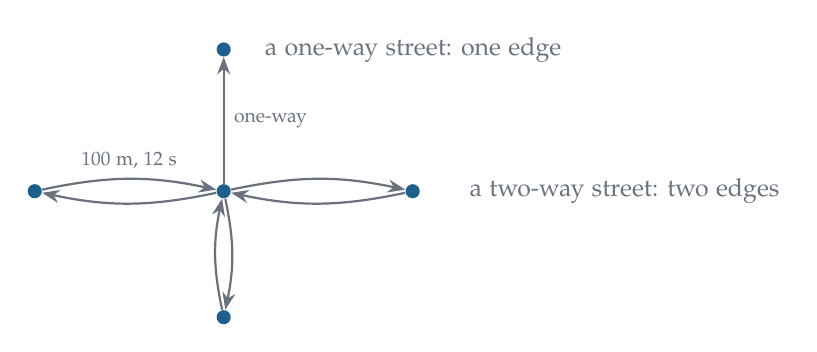
\begin{tikzpicture}[
  n/.style={circle, fill=accent, inner sep=1.8pt},
  e/.style={-{Stealth[length=2.2mm]}, thick, color=cm},
  lab/.style={font=\scriptsize, text=cm}]
  \node[n] (a) at (0,0) {};
  \node[n] (b) at (2.4,0) {};
  \node[n] (c) at (4.8,0) {};
  \node[n] (d) at (2.4,1.8) {};
  \node[n] (e) at (2.4,-1.6) {};
  \draw[e] (a) to[bend left=12] node[above, lab] {100 m, 12 s} (b);
  \draw[e] (b) to[bend left=12] (a);
  \draw[e] (b) to[bend left=12] (c);
  \draw[e] (c) to[bend left=12] (b);
  \draw[e] (b) -- node[right, lab] {one-way} (d);
  \draw[e] (e) to[bend left=12] (b);
  \draw[e] (b) to[bend left=12] (e);
  \node[font=\small, text=cm, anchor=west] at (5.4,0) {a two-way street: two edges};
  \node[font=\small, text=cm, anchor=west] at (2.8,1.8) {a one-way street: one edge};
\end{tikzpicture}
\end{center}

The same map gives different graphs to different travellers. A driver
can't use footpaths and must respect one-way streets. A walker can use
every road and path, in either direction. So the graph is built for a
\emph{mode} of travel: driving or walking.

\section{Speeds}

How fast does a traveller go? Real route planners use the speed limit of
each road, adjusted by the time of day and live traffic. We use one speed
for each kind of road: 60\,km/h on the main road, 40 on the lanes, 30 in
town and 20 on the bumpy tracks, while a walker goes at a steady
5\,km/h anywhere. A speed of 0 means the traveller can't use that kind of
road at all.

\begin{newfile}{road_graph.nex}
-- road_graph.nex: the roads as a graph, for one way of travelling.

intern Island_Map

-- How the traveller gets about.
enum union Mode
  Driving
  Walking
end

-- How fast a traveller goes on a kind of road, in km/h; 0 means the
-- traveller may not use it at all.
function speed_kmh(mode: Mode, kind: Road_Kind): Real do
  if mode = Mode.Walking then
    result := 5.0
  elseif kind = Road_Kind.Main then
    result := 60.0
  elseif kind = Road_Kind.Lane then
    result := 40.0
  elseif kind = Road_Kind.Street then
    result := 30.0
  elseif kind = Road_Kind.Track then
    result := 20.0
  else
    result := 0.0
  end
ensure
  non_negative: result >= 0.0
end
\end{newfile}

An edge knows its two nodes, its length, and the road it belongs to. The
time it takes is worked out once, when the edge is made: a speed of $v$
km/h is $v / 3.6$ metres per second (a kilometre is 1,000 metres and an
hour 3,600 seconds), and time is distance divided by speed.

\begin{append}{road_graph.nex}
-- One step of travel: from node `source` straight to the next node
-- along a road, `target`.
class Edge
create
  make(s, t: Integer, metres, kmh: Real, r: Road)
  require
    different_nodes: s /= t
    positive_length: metres > 0.0
    positive_speed: kmh > 0.0
  do
    source := s
    target := t
    length := metres
    seconds := metres / (kmh / 3.6)
    road := r
  end
feature
  once source: Integer
  once target: Integer
  -- How long the step is, in metres...
  once length: Real
  -- ...and how long it takes, in seconds.
  once seconds: Real
  -- The road the step is part of.
  once road: Road
end
\end{append}

\section{Building the graph}

How should a graph be stored? The question a route planner asks over and
over is ``where can I go from this node?'', so we store, for every node,
the list of edges leaving it. This is called an \emph{adjacency list}. A
map from node ids to arrays of edges does it.

To build the graph, go through every road the traveller may use, and every
pair of neighbouring nodes along it. Add the edge in the road's direction,
and, unless the road is one-way and the traveller is driving, the edge
back.

\begin{append}{road_graph.nex}
class Road_Graph
create
  -- The graph of the roads of `m` that a traveller can use in mode `how`.
  build(m: Island_Map, how: Mode) do
    island := m
    mode := how
    adjacency := {}
    edge_count := 0
    top_speed := 0.0
    across m.roads as r do
      let kmh: Real := speed_kmh(how, r.kind)
      if kmh > 0.0 then
        top_speed := top_speed.max(kmh / 3.6)
        let both_ways: Boolean := not r.is_one_way or how = Mode.Walking
        from
          let i: Integer := 1
        until
          i >= r.node_ids.length
        do
          let a: Integer := r.node_ids.get(i - 1)
          let b: Integer := r.node_ids.get(i)
          let metres: Real := m.point(a).distance_to(m.point(b))
          add_edge(create Edge.make(a, b, metres, kmh, r))
          if both_ways then
            add_edge(create Edge.make(b, a, metres, kmh, r))
          end
          i := i + 1
        end
      end
    end
  end
feature
  island: Island_Map
  mode: Mode
  -- For every node, the edges that leave it.
  adjacency: Map[Integer, Array[Edge]]
  edge_count: Integer
  -- The fastest speed on any edge, in metres per second.
  top_speed: Real
\end{append}

The graph also remembers the fastest speed on any of its edges. That will
be useful in Chapter~\ref{ch:astar}.

The questions the graph answers: is a node on its roads, which nodes it
has, which edges leave a node, and is there an edge from one node to
another. A node with no edges leaving it, such as the last node of a
one-way street that ends at nothing, is still a node of the graph, so
\code{add_edge} makes sure both ends are in the map.

\begin{continued}{road_graph.nex}
  -- Whether `id` is on a road this graph's traveller can use.
  has_node(id: Integer): Boolean do
    result := adjacency.contains_key(id)
  end

  -- Every node of the graph.
  nodes(): Array[Integer] do
    result := adjacency.keys
  end

  -- The edges leaving `id` (none if it is not in the graph).
  edges_from(id: Integer): Array[Edge] do
    result := adjacency.try_get(id, [])
  end

  -- The edge from a to b, if there is one.
  edge_between(a, b: Integer): ?Edge do
    across edges_from(a) as e do
      if e.target = b then
        result := e
      end
    end
  end
\end{continued}

\section{Joining the roads}

A place, or a point someone clicks on the map, is usually not on a road
at all. The harbour is at the water's edge, a little south of Quay
Street; the campsite is in a field at the end of a track. To plan a route
from it, we first join the roads at the nearest node, which is called
\emph{snapping}. The nearest node is simply the one at the smallest
distance; for the few hundred nodes of an island, checking them all is
instant. (A real map has hundreds of millions of nodes, and finds the
nearest with a \emph{spatial index}, which narrows the search to the
nodes in the same small square of the map.)

\begin{continued}{road_graph.nex}
  -- The node of the graph closest to p: where a traveller standing at p
  -- joins the roads.
  nearest_node(p: Point): Integer
  require
    not_empty: edge_count > 0
  do
    let best: Real := -1.0
    across adjacency.keys as id do
      let d: Real := island.point(id).distance_to(p)
      if best < 0.0 or d < best then
        best := d
        result := id
      end
    end
  ensure
    in_graph: has_node(result)
  end

private feature
  add_edge(e: Edge) do
    if not adjacency.contains_key(e.source) then
      adjacency.put(e.source, [])
    end
    -- A one-way road's last node has no edge leaving it, but it is still a
    -- node of the graph.
    if not adjacency.contains_key(e.target) then
      adjacency.put(e.target, [])
    end
    adjacency.get(e.source).add(e)
    edge_count := edge_count + 1
  end
invariant
  non_negative_count: edge_count >= 0
end
\end{continued}

Because the snapping is done in the traveller's own graph, a walker can be
snapped to a footpath, but a driver never is.

\section{Looking at a junction}

Where Harbour Street crosses Market Street, in the middle of town, four
stretches of road meet. Market Street is one-way, eastbound. This script
finds the node the two streets share and lists the edges leaving it, for a
driver and for a walker:

\begin{tryit}{try_graph.nex}
intern Road_Graph
intern Helpers

let island: Island_Map := create Island_Map.load(user_path("kestrel_island.map"))
let driving: Road_Graph := create Road_Graph.build(island, Mode.Driving)
let walking: Road_Graph := create Road_Graph.build(island, Mode.Walking)
console.print_line("driving: " + driving.nodes.length.to_string + " nodes, "
  + driving.edge_count.to_string + " edges")
console.print_line("walking: " + walking.nodes.length.to_string + " nodes, "
  + walking.edge_count.to_string + " edges")

-- The node that Harbour Street and Market Street share.
let crossing: Integer := 0
across island.roads as a do
  across island.roads as b do
    if a.name = "Harbour Street" and b.name = "Market Street" then
      across a.node_ids as id do
        if b.node_ids.contains(id) then
          crossing := id
        end
      end
    end
  end
end
across [driving, walking] as g do
  console.print_line("")
  console.print_line(g.mode.to_string + " from node " + crossing.to_string + ":")
  across g.edges_from(crossing) as e do
    console.print_line("  to node " + e.target.to_string.pad_end(" ", 4) + " along " + e.road.name
      + ", " + bearing(island.point(e.source), island.point(e.target)).round.to_string
      + " degrees, " + e.length.format(0) + " m, " + e.seconds.format(1) + " s")
  end
end
\end{tryit}
\tryoutput{try_graph}

A driver can leave the junction three ways: north and south on Harbour
Street, and east on Market Street. A walker has a fourth: west on Market
Street, against the traffic. The same 100 metres takes 12 seconds to
drive and 72 seconds to walk.

The walking graph has more nodes than the driving one, since it includes
the footpaths, and nearly twice as many edges per road, since every road
is two-way on foot.

% ===========================================================================
\chapter{The fewest steps: breadth-first search}\label{ch:bfs}

We have a graph. Now: what is the best way from one node to another? This
chapter and the next two answer that question three times, each time a
little better. All three algorithms share one idea. Starting from the
source, they explore the graph outwards, keeping a list of nodes they know
how to reach but haven't explored yet, called the \emph{frontier}. They
differ only in which frontier node they explore next.

\section{What a search finds}

Every search gives back the same kind of answer: the path it found, as a
list of nodes from the source to the target, and the total cost of that
path. It also gives back two things that describe its work, so that we can
compare the algorithms and draw them: the nodes it explored, in the order
it explored them, and how it reached each node.

That last part is the trick that makes all these searches cheap. When the
search first reaches node $n$ from node $m$, it writes down
``$n$ came from $m$'': $m$ is $n$'s \emph{parent}. It never needs to store
whole paths. When it reaches the target, it follows the parent links back
to the source, and that is the path, backwards.

\begin{newfile}{search.nex}
-- search.nex: finding a way from one node to another. Breadth-first
-- search, Dijkstra's algorithm and A*.

intern Road_Graph

-- What a search found, and how much work it did to find it.
class Search_Result
create
  make(name: String, nodes: Array[Integer], total: Real,
    order: Array[Integer], tree: Map[Integer, Integer]) do
    algorithm := name
    path := nodes
    cost := total
    explored := order
    parents := tree
  end
feature
  algorithm: String
  -- The nodes of the way found, from start to finish; empty if there is
  -- no way.
  path: Array[Integer]
  -- What the search was minimising, added up along the path.
  cost: Real
  -- Every node the search finished with, in the order it did so.
  explored: Array[Integer]
  -- How the search reached each node it saw: parents.get(n) is the node
  -- it came to n from. Together these links form a tree.
  parents: Map[Integer, Integer]

  found(): Boolean do
    result := not path.is_empty
  end
end

-- The way from `source` to `target`, following the parent links back
-- from `target` and then turning the list around.
function trace_back(parents: Map[Integer, Integer], source, target: Integer): Array[Integer] do
  let backwards: Array[Integer] := [target]
  let at: Integer := target
  from
  until
    at = source
  do
    at := parents.get(at)
    backwards.add(at)
  end
  result := backwards.reverse
ensure
  starts_at_source: result.get(0) = source
  ends_at_target: result.get(result.length - 1) = target
end
\end{newfile}

Two more helpers, which we'll use in contracts and checks: whether a list
of nodes really is a route through the graph (every step must be an
edge), and the total cost of a route, for any way of costing an edge.

\begin{append}{search.nex}
-- Whether `path` is a way through the graph: every step is an edge.
function is_route(g: Road_Graph, path: Array[Integer]): Boolean do
  result := not path.is_empty
  from
    let i: Integer := 1
  until
    not result or i >= path.length
  do
    result := g.edge_between(path.get(i - 1), path.get(i)) /= nil
    i := i + 1
  end
end

-- The total of `cost` over the steps of a route.
function route_cost(g: Road_Graph, path: Array[Integer], cost: Function(Edge): Real): Real
require
  is_a_route: is_route(g, path)
do
  from
    let i: Integer := 1
  until
    i >= path.length
  do
    if ?g.edge_between(path.get(i - 1), path.get(i)) as e then
      result := result + cost(e)
    end
    i := i + 1
  end
end
\end{append}

\code{route_cost}'s last parameter is a \emph{function}:
\code{Function(Edge): Real} is the type of a function that takes an edge
and gives back a number. Passing it in lets one routine add up lengths,
times, or anything else. Here are the two ways of costing an edge we will
use, each as a function that returns the costing function:

\begin{append}{search.nex}
-- Two ways to measure an edge: by its length, or by how long it takes.
function by_distance(): Function(Edge): Real do
  result := fn (e: Edge): Real do result := e.length end
end

function by_time(): Function(Edge): Real do
  result := fn (e: Edge): Real do result := e.seconds end
end
\end{append}

\code{fn (e: Edge): Real do ... end} is an \emph{anonymous function}: a
function written as a value, without a name. Inside it, \code{result} is
the anonymous function's own result.

\section{Breadth-first search}

The simplest search explores the frontier in the order it found it: first
in, first out, like a queue at a shop. Start with just the source in the
queue. Repeatedly take the node at the front of the queue; if it is the
target, stop; otherwise put each of its neighbours that hasn't been seen
before at the back of the queue, with the node as its parent.

\begin{center}
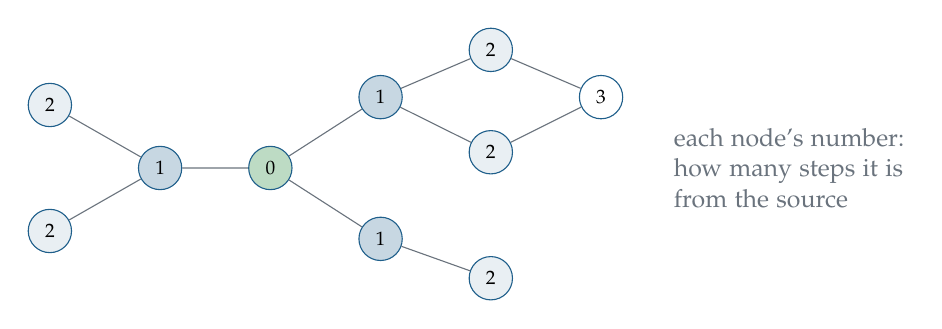
\begin{tikzpicture}[
  n/.style={circle, draw=accent, fill=white, inner sep=0pt, minimum size=5.5mm, font=\scriptsize},
  e/.style={color=cm}]
  \node[n, fill=st!30] (s) at (0,0) {0};
  \foreach \i/\x/\y in {a/1.4/0.9, b/1.4/-0.9, c/-1.4/0} \node[n, fill=accent!25] (\i) at (\x,\y) {1};
  \foreach \i/\x/\y in {d/2.8/1.5, f/2.8/0.2, g/2.8/-1.4, h/-2.8/0.8, k/-2.8/-0.8} \node[n, fill=accent!10] (\i) at (\x,\y) {2};
  \node[n] (m) at (4.2,0.9) {3};
  \draw[e] (s) -- (a) (s) -- (b) (s) -- (c) (a) -- (d) (a) -- (f) (b) -- (g) (c) -- (h) (c) -- (k) (d) -- (m) (f) -- (m);
  \node[font=\small, text=cm, align=left, anchor=west] at (5,0) {each node's number:\\how many steps it is\\from the source};
\end{tikzpicture}
\end{center}

Nodes come out of the queue in rings: the source, then every node one step
from it, then every node two steps away, and so on. A node is put in the
queue the first time it is seen, from a node one ring further in. So when
the target comes out, the parent links lead back to the source along a
path with \emph{the fewest steps} there is. That is what breadth-first
search finds.

Removing the first element of a Nex array shifts all the others down, so
instead of removing anything, we keep an index, \code{front}, of the next
node to take. The nodes before it have all been explored.

\begin{append}{search.nex}
-- Breadth-first search: the way with the fewest steps.
--
-- The search keeps a queue of nodes to visit, first in, first out. It
-- starts with just the source. It takes the node at the front of the
-- queue and puts every neighbour it has not seen before at the back, and
-- repeats until it takes out the target. Nodes come out in order of how
-- many steps they are from the source: all the nodes 1 step away, then
-- all those 2 steps away, and so on. So the first time the search reaches
-- the target, it has reached it in as few steps as possible.
function breadth_first(g: Road_Graph, source, target: Integer): Search_Result
require
  source_on_roads: g.has_node(source)
  target_on_roads: g.has_node(target)
do
  let queue: Array[Integer] := [source]
  let front: Integer := 0
  let seen: Set[Integer] := #{source}
  let parents: Map[Integer, Integer] := {}
  let explored: Array[Integer] := []
  let found: Boolean := false
  from
  until
    found or front = queue.length
  do
    let node: Integer := queue.get(front)
    front := front + 1
    explored.add(node)
    if node = target then
      found := true
    else
      across g.edges_from(node) as e do
        if not seen.contains(e.target) then
          seen.add(e.target)
          parents.put(e.target, node)
          queue.add(e.target)
        end
      end
    end
  end
  let path: Array[Integer] := []
  if found then
    path := trace_back(parents, source, target)
  end
  result := create Search_Result.make("breadth-first", path,
    (path.length - 1).max(0).to_real, explored, parents)
ensure
  valid_path: not result.found() or is_route(g, result.path)
end
\end{append}

If the queue runs out before the target turns up, the target can't be
reached, and the path is empty. The cost of a breadth-first path is its
number of steps.

The postcondition says that whatever the search finds is a real route:
``either nothing was found, or the path is a route''. It is checked every
time the search runs.

\section{Watching a search}

To see what the searches do, we'll draw them: the map, then a line from
every explored node to its parent in purple, which shows the part of the
graph the search covered, and the path it found in blue. This try-it file
holds the drawing code, and the next few chapters' try-its use it with
\code{intern Try_Pictures}.

\begin{tryit}{try_pictures.nex}
-- try_pictures.nex: drawing a search on the map, for the try-its of the
-- next few chapters.

intern Map_View
intern Search
intern Helpers

-- Draw the map, then the part of the graph that `found` explored in
-- purple, then the way it found in blue, and save the picture.
function picture_of_search(view: Map_View, found: Search_Result, file: String) do
  let island: Island_Map := view.island
  view.draw_map()
  view.set_pen(create Color.make_rgba(150, 60, 200, 170), 4.0)
  across found.explored as n do
    if found.parents.contains_key(n) then
      let a: Point := island.point(found.parents.get(n))
      let b: Point := island.point(n)
      view.canvas.line(a.x, a.y, b.x, b.y)
    end
  end
  view.line(island.points_of(found.path), create Color.make(40, 110, 220), 5.0)
  view.save(file)
end

-- A one-line summary of a search, for driving.
function summary(g: Road_Graph, found: Search_Result): String do
  result := found.algorithm + ": " + found.explored.length.to_string + " nodes explored, "
    + (found.path.length - 1).to_string + " steps, "
    + distance_text(route_cost(g, found.path, by_distance())) + ", "
    + duration_text(route_cost(g, found.path, by_time()))
end
\end{tryit}

Now a search from the beach car park, on the south-west coast, to the
lighthouse, on the northern cape. A place isn't a node of the graph, so we
snap each one to its nearest node first.

\begin{tryit}{try_bfs.nex}
intern Try_Pictures

let island: Island_Map := create Island_Map.load(user_path("kestrel_island.map"))
let g: Road_Graph := create Road_Graph.build(island, Mode.Driving)
if ?island.find_place("beach") as a and ?island.find_place("lighthouse") as b then
  let source: Integer := g.nearest_node(island.point(a.node_id))
  let target: Integer := g.nearest_node(island.point(b.node_id))
  let found: Search_Result := breadth_first(g, source, target)
  console.print_line(summary(g, found))
  picture_of_search(create Map_View.make(island, 1000, 700), found, "bfs.png")
end
\end{tryit}
\tryoutput{try_bfs}
\mappicture{bfs}

The purple spreads out evenly in every direction from the car park, along
every road, until it touches the lighthouse. The path it found goes all the
way round the west of the island on the Coast Road.

Is that the best way? It is the way with the fewest steps, but a step is
not a fixed distance. Look back at the map file: the nodes along the Coast
Road are about 320 metres apart, while the lanes have one every 170 metres
or so, and the town's streets one every 100. So a route along the Coast
Road has few, long steps, and breadth-first search likes it for that
reason alone. The road up the middle of the island, by Lake Road and Hill
Road, is shorter in metres, but it has more steps.

Breadth-first search is the right tool when every step costs the same,
like moves in a puzzle or links between web pages. Roads are not like
that. We need a search that counts metres, or seconds.

% ===========================================================================
\chapter{The cheapest way: Dijkstra's algorithm}\label{ch:dijkstra}

In 1956, Edsger Dijkstra, a young Dutch programmer, wanted a problem to
show off a new computer to people who knew nothing about computers. He
chose finding the shortest route between two cities in the Netherlands,
and, sitting at a café, worked out how to do it in twenty minutes. His
algorithm is still at the heart of every route planner.

\section{The idea}

Breadth-first search explores the frontier in the order it found it. In
Dijkstra's algorithm, every frontier node also carries the cost of the
cheapest way to it found so far, and the search always explores the
\emph{cheapest} frontier node next.

When the search explores node $n$, it looks at every edge from $n$ to a
neighbour $m$. The way to $m$ through $n$ costs the way to $n$, plus the
edge. If that is cheaper than any way to $m$ found before (or $m$ hasn't
been seen at all), it becomes $m$'s best known way: $m$ gets that cost,
and $n$ as its parent.

\begin{mathbox}[Why the cheapest frontier node is finished]
Say node $n$ is the cheapest on the frontier, with cost $c$. Could there
be a cheaper way to $n$ that the search hasn't found yet? Any such way
starts at the source, inside the explored region, and must leave the
region at some point, through some frontier node $f$. The way to $f$
already costs at least $c$, because $n$ was the cheapest on the frontier,
and the rest of the way from $f$ to $n$ can only add to that, since no edge
costs less than nothing. So no way to $n$ costs less than $c$, and $n$'s
best way is final. The search can explore it, and never look at it again.
\end{mathbox}

So the explored region grows in order of cost, like a ring of water
spreading from a stone dropped in a pond, except that the ripple runs
fast along cheap roads and slowly along expensive ones. When the target is
explored, its cost is final, and following its parents gives the cheapest
way there.

The argument needs one thing: no edge may have a negative cost. Lengths
and travel times never do.

\section{A priority queue}

``Take the cheapest frontier node'' could be done by looking through the
whole frontier every time, but there is a data structure made for it: a
\emph{priority queue}, which hands out its items smallest first. Nex has
one built in, \code{Min_Heap}. Adding an item and taking out the smallest
both take a time proportional to $\log n$ for $n$ items, instead of $n$.

What goes in the queue is a node with its cost, and its \emph{priority}:
the number the queue sorts by. For Dijkstra's algorithm the priority is
just the cost; in the next chapter it won't be. A \code{Min_Heap} of our
own class needs to be told how to compare two items: a function that gives
a negative number when the first comes first, positive when it comes
second, and 0 when they tie. \code{Real}'s \code{compare} does exactly that.

\begin{append}{search.nex}
-- A node waiting to be explored, with the cost of the best way to it
-- found so far, and its priority: the lower, the sooner it is explored.
class Waiting
create
  make(n: Integer, c, p: Real) do
    node := n
    cost := c
    priority := p
  end
feature
  once node: Integer
  once cost: Real
  once priority: Real
end

-- Lower priority first.
function by_priority(): Function(Waiting, Waiting): Integer do
  result := fn (a, b: Waiting): Integer do result := a.priority.compare(b.priority) end
end
\end{append}

A priority queue doesn't let us change the cost of an item already in it,
which we would need when a cheaper way to a waiting node turns up. Instead
we simply add the node again, with its new cost. The cheaper copy comes out
first; when the old, dearer copy comes out later, the node is already
finished, and we skip it. This is called \emph{lazy deletion}, and it is
the usual way to do it.

\section{The algorithm}

\begin{append}{search.nex}
-- Dijkstra's algorithm: the way with the lowest total cost, where `cost`
-- gives the cost of each edge (its length, or the time it takes).
--
-- Like breadth-first search, but the queue is a priority queue: the next
-- node out is always the one with the cheapest way to it found so far.
-- When a node comes out, no cheaper way to it can turn up later, because
-- any other way would have to go through a node still waiting, and every
-- one of those is already at least as expensive. So the node is finished.
function dijkstra(g: Road_Graph, source, target: Integer,
  cost: Function(Edge): Real): Search_Result
require
  source_on_roads: g.has_node(source)
  target_on_roads: g.has_node(target)
do
  let waiting: Min_Heap[Waiting] := create Min_Heap[Waiting].from_comparator(by_priority())
  waiting.insert(create Waiting.make(source, 0.0, 0.0))
  let best: Map[Integer, Real] := {source: 0.0}
  let parents: Map[Integer, Integer] := {}
  let finished: Set[Integer] := #{}
  let explored: Array[Integer] := []
  let found: Boolean := false
  from
  until
    found or waiting.is_empty
  do
    let w: Waiting := waiting.extract_min
    -- A node can be in the queue more than once, if a cheaper way to it
    -- turned up after it was first added. Only its first time out counts.
    if not finished.contains(w.node) then
      finished.add(w.node)
      explored.add(w.node)
      if w.node = target then
        found := true
      else
        across g.edges_from(w.node) as e do
          let c: Real := w.cost + cost(e)
          if not best.contains_key(e.target) or c < best.get(e.target) then
            best.put(e.target, c)
            parents.put(e.target, w.node)
            waiting.insert(create Waiting.make(e.target, c, c))
          end
        end
      end
    end
  end
  let path: Array[Integer] := []
  if found then
    path := trace_back(parents, source, target)
  end
  result := create Search_Result.make("Dijkstra", path,
    best.try_get(target, 0.0), explored, parents)
ensure
  valid_path: not result.found() or is_route(g, result.path)
  cost_adds_up: not result.found()
    or (route_cost(g, result.path, cost) - result.cost).abs < 0.001
end
\end{append}

Compare it with \code{breadth_first}: the shape is the same, a loop that
takes a node from the frontier and looks at its edges. The queue has become
a priority queue, \code{seen} has become \code{best}, which remembers a
cost for every node seen, and a node is finished when it comes \emph{out}
of the queue, not when it goes in.

The second postcondition checks the algorithm's bookkeeping against an
independent calculation: adding up the cost of each edge along the path
found must give the cost the search reports.

\section{Shortest or quickest?}

The cost function decides what ``best'' means. With \code{by_distance()},
Dijkstra's algorithm finds the shortest route; with \code{by_time()}, the
quickest.

\begin{tryit}{try_dijkstra.nex}
intern Try_Pictures

let island: Island_Map := create Island_Map.load(user_path("kestrel_island.map"))
let g: Road_Graph := create Road_Graph.build(island, Mode.Driving)
if ?island.find_place("beach") as a and ?island.find_place("lighthouse") as b then
  let source: Integer := g.nearest_node(island.point(a.node_id))
  let target: Integer := g.nearest_node(island.point(b.node_id))
  let shortest: Search_Result := dijkstra(g, source, target, by_distance())
  say("shortest  " + summary(g, shortest))
  let quickest: Search_Result := dijkstra(g, source, target, by_time())
  say("quickest  " + summary(g, quickest))
  picture_of_search(create Map_View.make(island, 1000, 700), shortest, "dijkstra.png")
end
\end{tryit}
\tryoutput{try_dijkstra}
\mappicture{dijkstra}

The shortest way goes up the middle of the island: Lake Road, then Hill
Road, then Lighthouse Lane, 3.4 km. The quickest goes round the west coast
on the Coast Road. It is 700 metres longer, but the Coast Road is a 60\,km/h
road, against 40 for the lanes, and that more than makes up for it. Real
navigators nearly always plan the quickest route, and that is what our
navigator will do too.

Breadth-first search found the quickest route as well, but only by luck:
the Coast Road happens to have both few steps and fast ones.

Look at the purple, though. Dijkstra's algorithm explored most of
the island to find a route to its northern tip, including the whole of the
town in the south, which is in exactly the wrong direction. It has no
idea where the lighthouse is; it only knows what things cost. The next
chapter gives it a sense of direction.

% ===========================================================================
\chapter{A sense of direction: A*}\label{ch:astar}

Dijkstra's algorithm explores in order of cost so far, so it spreads in
every direction alike. But we know where the target is. A node a kilometre
from the source and two from the target is a better bet than one a
kilometre from the source and five from the target. In 1968 Peter Hart,
Nils Nilsson and Bertram Raphael, building a robot called Shakey at the
Stanford Research Institute, turned that thought into an algorithm, and
called it A*.

\section{The idea}

A* is Dijkstra's algorithm with one change: the priority of a frontier
node $n$ is not just $g(n)$, the cost of the best way to it so far, but
\[
  f(n) = g(n) + h(n),
\]
where $h(n)$ is an \emph{estimate} of the cost still to come, from $n$ to
the target. $f(n)$ is an estimate of the cost of the whole route through
$n$. Nodes on the way to the target have low estimates, so they come out of
the queue early; nodes leading away have high ones, and wait, very often
until the target has been found and the search is over.

That raises a worry. Dijkstra's algorithm is right because it explores
nodes in order of their true cost. If the estimate pushes a node to the
front of the queue, could A* finish the target before finding its cheapest
way? Not if the estimate is never too high.

\begin{mathbox}[When A* finds the best route]
Call an estimate \emph{admissible} if it never overestimates:
$h(n)$ is at most the true cost of the cheapest way from $n$ to the
target. When the target $t$ comes out of the queue, its priority is
$f(t) = g(t) + 0$, the cost of the route found. Every node $m$ still in the
queue has $f(m) \ge f(t)$, and $f(m)$ is \emph{at most} the cost of the
best route through $m$, since $h(m)$ doesn't overestimate. So no route
through any waiting node can be cheaper than the one found.

Our estimates have a slightly stronger property, called being
\emph{consistent}: for every edge from $n$ to $m$, $h(n) \le
\text{cost}(n, m) + h(m)$. The estimate never drops by more than the edge
costs. With a consistent estimate, a node is also finished the first time
it comes out of the queue, exactly as in Dijkstra's algorithm, so the same
code works.
\end{mathbox}

With $h(n) = 0$ for every node, A* is Dijkstra's algorithm. The better the
estimate, the fewer nodes A* explores; a perfect estimate would lead it
straight to the target without a single wasted step.

\section{Estimates}

When the cost is distance, the obvious estimate is the straight-line
distance to the target. No road between two points is shorter than the
straight line between them, so it never overestimates. And it is
consistent, because of the \emph{triangle inequality}: going from $n$
straight to the target is never longer than going from $n$ to $m$ and then
straight to the target.

When the cost is time, the straight-line distance must be turned into a
time that is never too much. Dividing it by the fastest speed on any road
does it: no trip can be quicker than travelling the straight line at top
speed all the way. That is what the graph's \code{top_speed} is for.

Each estimate is a function from a node to a number, built for one target.
Note how the anonymous function uses \code{goal} and \code{speed}, which
are local variables of the function that made it. The anonymous function
\emph{captures} them, and keeps them for as long as it lives, after
\code{time_estimate} itself has returned. A function value with captured
variables is called a \emph{closure}.

\begin{append}{search.nex}
-- A straight-line estimate of the cost from any node to `target`, when
-- the cost is distance: no road between two points is shorter than the
-- straight line between them.
function distance_estimate(g: Road_Graph, target: Integer): Function(Integer): Real do
  let goal: Point := g.island.point(target)
  result := fn (n: Integer): Real do
    result := g.island.point(n).distance_to(goal)
  end
end

-- The same when the cost is time: no trip is quicker than the straight
-- line at the top speed of any road.
function time_estimate(g: Road_Graph, target: Integer): Function(Integer): Real do
  let goal: Point := g.island.point(target)
  let speed: Real := g.top_speed
  result := fn (n: Integer): Real do
    result := g.island.point(n).distance_to(goal) / speed
  end
end
\end{append}

\section{The algorithm}

Here is A*. The only differences from \code{dijkstra} are the extra
parameter, \code{estimate}, and the priority given to each node added to
the queue: \code{c + estimate(e.target)} instead of \code{c}.

\begin{append}{search.nex}
-- A* ("A star"): Dijkstra's algorithm with a sense of direction.
--
-- The priority of a waiting node is the cost of the best way to it so
-- far, plus an estimate of the cost from it to the target. Nodes that
-- lead towards the target come out sooner, and nodes that lead away wait,
-- often until the target is found and they are never explored at all.
-- As long as the estimate is never more than the true cost, the way A*
-- finds is just as cheap as the one Dijkstra finds.
function a_star(g: Road_Graph, source, target: Integer,
  cost: Function(Edge): Real, estimate: Function(Integer): Real): Search_Result
require
  source_on_roads: g.has_node(source)
  target_on_roads: g.has_node(target)
do
  let waiting: Min_Heap[Waiting] := create Min_Heap[Waiting].from_comparator(by_priority())
  waiting.insert(create Waiting.make(source, 0.0, estimate(source)))
  let best: Map[Integer, Real] := {source: 0.0}
  let parents: Map[Integer, Integer] := {}
  let finished: Set[Integer] := #{}
  let explored: Array[Integer] := []
  let found: Boolean := false
  from
  until
    found or waiting.is_empty
  do
    let w: Waiting := waiting.extract_min
    if not finished.contains(w.node) then
      finished.add(w.node)
      explored.add(w.node)
      if w.node = target then
        found := true
      else
        across g.edges_from(w.node) as e do
          let c: Real := w.cost + cost(e)
          if not best.contains_key(e.target) or c < best.get(e.target) then
            best.put(e.target, c)
            parents.put(e.target, w.node)
            waiting.insert(create Waiting.make(e.target, c, c + estimate(e.target)))
          end
        end
      end
    end
  end
  let path: Array[Integer] := []
  if found then
    path := trace_back(parents, source, target)
  end
  result := create Search_Result.make("A*", path,
    best.try_get(target, 0.0), explored, parents)
ensure
  valid_path: not result.found() or is_route(g, result.path)
  cost_adds_up: not result.found()
    or (route_cost(g, result.path, cost) - result.cost).abs < 0.001
end
\end{append}

We could have written \code{dijkstra} as a call to \code{a_star} with an
estimate of zero. Keeping both, side by side, makes it easy to see how
little separates them.

Last, one function that chooses an algorithm by name and plans the
quickest route, or the shortest. The programs at the end of the tutorial
use it, so that you can switch algorithms while they run.

\begin{append}{search.nex}
-- Search with the algorithm called `algorithm` ("bfs", "dijkstra" or
-- "astar"), for the quickest way, or the shortest one if `shortest`.
function find_route(g: Road_Graph, source, target: Integer, algorithm: String,
  shortest: Boolean): Search_Result
require
  source_on_roads: g.has_node(source)
  target_on_roads: g.has_node(target)
  known_algorithm: algorithm = "bfs" or algorithm = "dijkstra" or algorithm = "astar"
do
  let cost: Function(Edge): Real := when shortest then by_distance() else by_time() end
  let estimate: Function(Integer): Real :=
    when shortest then distance_estimate(g, target) else time_estimate(g, target) end
  if algorithm = "bfs" then
    result := breadth_first(g, source, target)
  elseif algorithm = "dijkstra" then
    result := dijkstra(g, source, target, cost)
  else
    result := a_star(g, source, target, cost, estimate)
  end
end
\end{append}

\section{Dijkstra against A*}

\begin{tryit}{try_astar.nex}
intern Try_Pictures

let island: Island_Map := create Island_Map.load(user_path("kestrel_island.map"))
let g: Road_Graph := create Road_Graph.build(island, Mode.Driving)
if ?island.find_place("beach") as a and ?island.find_place("lighthouse") as b then
  let source: Integer := g.nearest_node(island.point(a.node_id))
  let target: Integer := g.nearest_node(island.point(b.node_id))
  console.print_line(summary(g, dijkstra(g, source, target, by_time())))
  let found: Search_Result := a_star(g, source, target, by_time(), time_estimate(g, target))
  console.print_line(summary(g, found))
  picture_of_search(create Map_View.make(island, 1000, 700), found, "astar.png")
end

console.print_line("")
console.print_line("Nodes explored for the quickest route by car:")
across [["harbour", "lighthouse"], ["campsite", "fisher"], ["school", "peak"],
    ["mill", "beach"]] as trip do
  if ?island.find_place(trip.get(0)) as a and ?island.find_place(trip.get(1)) as b then
    let s: Integer := g.nearest_node(island.point(a.node_id))
    let t: Integer := g.nearest_node(island.point(b.node_id))
    console.print_line("  " + (a.name + " to " + b.name).pad_end(" ", 34)
      + dijkstra(g, s, t, by_time()).explored.length.to_string.pad_start(" ", 4)
      + a_star(g, s, t, by_time(), time_estimate(g, t)).explored.length.to_string.pad_start(" ", 5))
  end
end
\end{tryit}
\tryoutput{try_astar}
\mappicture{astar}

A* finds the same route as Dijkstra's algorithm, exactly as quick, but
explores less than half as many nodes: the purple now leans towards the
lighthouse, and most of the town, off to the east of the car park, is
left alone.

The other trips show that the saving varies. From the mill to the beach,
A* explores a fifth as many nodes as Dijkstra's algorithm. But from the
school to Kestrel Peak it saves hardly anything. The quickest way to the
peak ends on the slow tracks through the wood, and the estimate, which
assumes 60\,km/h all the way, is far below the true time. When the
estimate is that far off, A* has little to go on, and behaves almost like
Dijkstra's algorithm.

That is the general rule: the closer the estimate is to the truth, the
less A* explores. Our estimate for time is cautious, because it has to be:
it must never be too high, so it assumes the top speed everywhere. When
walking, every road has the same speed, so the straight-line estimate is
much closer to the truth, and A* is even more focused. The checks in the next chapter compare the two over every pair of
places.

% ===========================================================================
\chapter{Trust, but verify}\label{ch:checks}

Route planning is the kind of code where a bug hides well. A search that
is wrong now and then still finds a route every time, and the route still
looks reasonable on the map; it is just not quite the best one, for some
pairs of places. Nobody notices until somebody does.

Our contracts already check every single call: every path found is a real
route, its cost adds up, every projection goes back where it came from.
What contracts can't easily say is how different parts relate to each
other, or what should be true of the map as a whole. So the last file of
the core gets a set of \emph{checks}: a program that tests properties we
know must hold, over every pair of places on the island, for both drivers
and walkers.

\section{A checker}

A checker counts what passes and what fails, and prints each result. At
the end it prints a summary, and if anything failed it stops the program
with a non-zero exit code, the signal that scripts and build tools look
for.

\begin{newfile}{checks.nex}
-- checks.nex: executable checks for every piece of the project.
-- Run: nex checks.nex

intern Search
intern Helpers

class Checker
feature
  passed: Integer
  failed: Integer

  check(label: String, ok: Boolean) do
    if ok then
      passed := passed + 1
      say("PASS " + label)
    else
      failed := failed + 1
      say("FAIL " + label)
    end
  end

  close_to(label: String, expected, actual, tolerance: Real) do
    check(label + " (expected " + fixed(expected, 3) + ", got " + fixed(actual, 3) + ")",
      (expected - actual).abs <= tolerance)
  end

  summary() do
    say("---")
    say(passed.to_string + " passed, " + failed.to_string + " failed")
    if failed > 0 then
      exit(1)
    end
  end
end

function pt(x, y: Real): Point do
  result := create Point.make(x, y)
end
\end{newfile}

\code{close_to} is for numbers worked out with \code{Real}s, which are
rarely exactly equal to what we expect, because of rounding. It passes if
the two are within a given tolerance.

\section{The basics}

The first checks are of the helpers, the geography and the geometry. Each
compares a result with an answer we know independently: one degree of
latitude is $2\pi R / 360$; a 10-metre square has an area of 100; the
point 5 metres along a line that goes 3 metres east and then 4 north is
2 metres up its second segment.

\begin{append}{checks.nex}
function check_helpers(c: Checker) do
  c.check("fixed rounds", fixed(2.345, 2) = "2.35" and fixed(-0.5, 1) = "-0.5")
  c.check("distance_text", distance_text(347.0) = "350 m" and distance_text(1234.0) = "1.2 km")
  c.check("duration_text", duration_text(20.0) = "under a minute"
    and duration_text(150.0) = "3 min" and duration_text(3900.0) = "1 h 05 min")
end

function check_geo(c: Checker) do
  let a: Lat_Lon := create Lat_Lon.make(47.0, -34.0)
  let b: Lat_Lon := create Lat_Lon.make(48.0, -34.0)
  -- A degree of latitude is 1/360 of a circle around the Earth.
  c.close_to("one degree of latitude, in metres", 2.0 * Real.PI * Earth.RADIUS / 360.0,
    a.distance_to(b), 0.01)
  c.close_to("distance is symmetric", a.distance_to(b), b.distance_to(a), 0.000001)
  let p: Projection := create Projection.make(a)
  let q: Lat_Lon := create Lat_Lon.make(47.02, -33.97)
  c.close_to("projection keeps distances, a few km from the centre", a.distance_to(q),
    p.to_point(a).distance_to(p.to_point(q)), a.distance_to(q) * 0.001)
  let back: Lat_Lon := p.to_lat_lon(p.to_point(q))
  c.close_to("projection round trip", 0.0, back.distance_to(q), 0.001)
  c.check("east is +x, north is +y", p.to_point(q).x > 0.0 and p.to_point(q).y > 0.0)
end

function check_geometry(c: Checker) do
  let square: Array[Point] := [pt(0.0, 0.0), pt(10.0, 0.0), pt(10.0, 10.0), pt(0.0, 10.0)]
  c.close_to("area of a 10 m square", 100.0, polygon_area(square), 0.000001)
  c.check("inside the square", polygon_contains(square, pt(5.0, 5.0)))
  c.check("outside the square", not polygon_contains(square, pt(15.0, 5.0))
    and not polygon_contains(square, pt(-1.0, 5.0)))
  c.close_to("distance to a segment, beside it", 5.0,
    distance_to_segment(pt(5.0, 5.0), pt(0.0, 0.0), pt(10.0, 0.0)), 0.000001)
  c.close_to("distance to a segment, past its end", 5.0,
    distance_to_segment(pt(13.0, 4.0), pt(0.0, 0.0), pt(10.0, 0.0)), 0.000001)
  c.check("bearings", bearing(pt(0.0, 0.0), pt(0.0, 1.0)) = 0.0
    and bearing(pt(0.0, 0.0), pt(1.0, 0.0)) = 90.0
    and bearing(pt(0.0, 0.0), pt(0.0, -1.0)) = 180.0
    and bearing(pt(0.0, 0.0), pt(-1.0, 0.0)) = 270.0)
  c.check("turn angles wrap around north", turn_angle(350.0, 10.0) = 20.0
    and turn_angle(10.0, 350.0) = -20.0 and turn_angle(0.0, 180.0) = 180.0)
  c.check("compass names", compass_name(0.0) = "north" and compass_name(100.0) = "east"
    and compass_name(350.0) = "north")
  let line: Array[Point] := [pt(0.0, 0.0), pt(3.0, 0.0), pt(3.0, 4.0)]
  c.close_to("line length", 7.0, line_length(line), 0.000001)
  c.close_to("point along a line", 2.0, point_along(line, 5.0).y, 0.000001)
end
\end{append}

\section{The map and its graphs}

Next, the map. Every place should be on land, and not in the lake; the
middle of the lake should be water; a point out at sea should be in no
area at all. And the graphs should obey the rules of the road: Market
Street is one-way, eastbound, so the driving graph must not have an edge
going west along it, while the walking graph must; and no footpath may
appear in the driving graph.

\begin{append}{checks.nex}
function check_map(c: Checker, m: Island_Map) do
  c.check("map loaded", m.name = "Kestrel Island" and m.places.length = 10
    and m.roads.length > 0 and m.areas.length > 0)
  let all_on_land: Boolean := true
  across m.places as p do
    if ?m.area_at(m.point(p.node_id)) as a then
      if a.kind = "water" then
        all_on_land := false
      end
    else
      all_on_land := false
    end
  end
  c.check("every place is on land", all_on_land)
  let lake_centre: Point := pt(0.0, 0.0)
  across m.areas as a do
    if a.kind = "water" then
      lake_centre := average(m.points_of(a.node_ids))
    end
  end
  if ?m.area_at(lake_centre) as a then
    c.check("the middle of the lake is water", a.kind = "water")
  else
    c.check("the middle of the lake is water", false)
  end
  c.check("out at sea is no area", m.area_at(pt(m.max_x() + 100.0, 0.0)) = nil)
  c.check("find_place by part of a name", ?m.find_place("mill") as p and p.name = "Old Mill")
end

function check_graphs(c: Checker, m: Island_Map, driving, walking: Road_Graph) do
  c.check("walking can use more roads than driving", walking.edge_count > driving.edge_count)
  -- Market Street is one-way, eastbound.
  let eastward: Boolean := true
  let westward_on_foot: Boolean := false
  across m.roads as r do
    if r.name = "Market Street" then
      across driving.edges_from(r.node_ids.get(1)) as e do
        if e.road.name = "Market Street" and e.target = r.node_ids.get(0) then
          eastward := false
        end
      end
      across walking.edges_from(r.node_ids.get(1)) as e do
        if e.road.name = "Market Street" and e.target = r.node_ids.get(0) then
          westward_on_foot := true
        end
      end
    end
  end
  c.check("cars may not drive the wrong way up a one-way street", eastward)
  c.check("walkers may", westward_on_foot)
  let no_footpaths: Boolean := true
  across driving.nodes as id do
    across driving.edges_from(id) as e do
      if e.road.kind = Road_Kind.Footpath then
        no_footpaths := false
      end
    end
  end
  c.check("no footpaths in the driving graph", no_footpaths)
end
\end{append}

\section{The searches}

Now the important ones. For every pair of places, and for drivers and
walkers alike, we run every search, and check:

\begin{itemize}[nosep]
  \item \textbf{Every place can reach every other.} With one-way streets,
    it is easy to make a map where a car can get into a street but never
    out. A real map gets this wrong surprisingly often.
  \item \textbf{A* agrees with Dijkstra's algorithm}, for the quickest
    routes and for the shortest. This is what A*'s mathematics promises,
    and if our estimate were ever too high, it is where we would see it.
  \item \textbf{Breadth-first search finds the fewest steps}: no route the
    others find has fewer.
  \item \textbf{The estimates never overshoot}: the estimate from the
    start is never more than the true cost.
  \item \textbf{A* does less work}, over all the pairs together.
  \item \textbf{The triangle inequality}: for any three places $a$, $b$
    and $x$, the shortest way from $a$ to $b$ is no longer than the
    shortest way from $a$ to $x$ plus the shortest from $x$ to $b$. If it
    ever were, the way through $x$ would be a shorter way from $a$ to $b$
    that the search had missed.
\end{itemize}

That is 100 pairs of places (each place to itself included) and five
searches for each, twice over: a thousand searches. They take a few
seconds.

\begin{append}{checks.nex}
-- The node a traveller in graph g starts from to go to or from a place.
function node_of(g: Road_Graph, p: Place): Integer do
  result := g.nearest_node(g.island.point(p.node_id))
end

function check_searches(c: Checker, m: Island_Map, g: Road_Graph, label: String) do
  -- Shortest distances between every pair of places, for the triangle
  -- check below.
  let dist: Map[String, Real] := {}
  let all_found: Boolean := true
  let same_time: Boolean := true
  let same_distance: Boolean := true
  let bfs_fewest: Boolean := true
  let admissible: Boolean := true
  let a_star_work: Integer := 0
  let dijkstra_work: Integer := 0
  across m.places as a do
    across m.places as b do
      let s: Integer := node_of(g, a)
      let t: Integer := node_of(g, b)
      let fast: Search_Result := dijkstra(g, s, t, by_time())
      let fast_a: Search_Result := a_star(g, s, t, by_time(), time_estimate(g, t))
      let short: Search_Result := dijkstra(g, s, t, by_distance())
      let short_a: Search_Result := a_star(g, s, t, by_distance(), distance_estimate(g, t))
      let fewest: Search_Result := breadth_first(g, s, t)
      all_found := all_found and fast.found() and short.found() and fewest.found()
      same_time := same_time and (fast.cost - fast_a.cost).abs < 0.001
      same_distance := same_distance and (short.cost - short_a.cost).abs < 0.001
      bfs_fewest := bfs_fewest and fewest.path.length <= short.path.length
        and fewest.path.length <= fast.path.length
      admissible := admissible and time_estimate(g, t)(s) <= fast.cost + 0.001
        and distance_estimate(g, t)(s) <= short.cost + 0.001
      a_star_work := a_star_work + fast_a.explored.length
      dijkstra_work := dijkstra_work + fast.explored.length
      dist.put(a.name + ">" + b.name, short.cost)
    end
  end
  c.check(label + ": every place can reach every other", all_found)
  c.check(label + ": A* finds routes as quick as Dijkstra's", same_time)
  c.check(label + ": A* finds routes as short as Dijkstra's", same_distance)
  c.check(label + ": breadth-first search finds the fewest steps", bfs_fewest)
  c.check(label + ": the estimates never overshoot", admissible)
  c.check(label + ": A* explores fewer nodes than Dijkstra ("
    + a_star_work.to_string + " against " + dijkstra_work.to_string + ")",
    a_star_work < dijkstra_work)
  let triangle: Boolean := true
  across m.places as a do
    across m.places as b do
      across m.places as x do
        triangle := triangle and dist.get(a.name + ">" + b.name)
          <= dist.get(a.name + ">" + x.name) + dist.get(x.name + ">" + b.name) + 0.001
      end
    end
  end
  c.check(label + ": no detour through a third place is shorter", triangle)
end
\end{append}

\code{time_estimate(g, t)(s)} makes the estimate function for target
\code{t} and calls it straight away, on \code{s}.

The shortest distances are remembered in a \code{Map} with keys like
\code{"Old Mill>Lighthouse"}, so the triangle check, with its thousand
combinations, needs no more searches.

Last, the program itself:

\begin{append}{checks.nex}
function main() do
  let c: Checker := create Checker
  let m: Island_Map := create Island_Map.load(user_path("kestrel_island.map"))
  let driving: Road_Graph := create Road_Graph.build(m, Mode.Driving)
  let walking: Road_Graph := create Road_Graph.build(m, Mode.Walking)
  check_helpers(c)
  check_geo(c)
  check_geometry(c)
  check_map(c, m)
  check_graphs(c, m, driving, walking)
  check_searches(c, m, driving, "driving")
  check_searches(c, m, walking, "walking")
  c.summary()
end

main()
\end{append}

\runoutput{checks.nex}{checks_core}

Everything passes. Look at the work done: over all the pairs, A* explores
about half as many nodes as Dijkstra's algorithm for drivers, and about a
third for walkers, for whom the straight-line estimate is closer to the
truth, just as the last chapter said.

Run the checks again whenever you change anything: the map file, a speed,
an algorithm. If you break something, a line saying \code{FAIL} tells you
what.

Try it. In \code{time_estimate}, divide by \code{speed / 2.0} instead of
\code{speed}, so that the estimate is twice what it should be, and run the
checks again. They don't even get as far as the search checks:

\begin{textout}
Error: Postcondition violation: cost_adds_up
  a_star, called ... in check_searches, does not deliver its postcondition
  `cost_adds_up`.
\end{textout}

With an estimate that is too high, A* can finish a node before it has found
the cheapest way to it. When the cheaper way turns up later, the search
gives the node a new parent and a new cost, but the nodes it already
reached from it keep the costs they got through the old way. The path
traced back through the parents then no longer costs what the search
says it does, and \code{a_star}'s own postcondition catches the
contradiction the first time it happens, long before anyone could notice a
slightly wrong route on the map. Put \code{speed} back, and everything
passes again.

% ===========================================================================
\chapter{Turn by turn}\label{ch:directions}

A route is a list of nodes: from the beach car park to the lighthouse, a
couple of dozen of them. Nobody wants to hear about nodes. They want to
hear ``Head west on Coast Road. After 3.8 km, turn left onto Lighthouse
Lane.'' This chapter turns routes into instructions, and then into the
first complete program of the project.

\section{Where to say something}

Most nodes of a route need no instruction at all: the traveller just keeps
going along the same road. Something needs saying only where the road
changes. So we walk along the route, edge by edge, and cut it into
\emph{stretches}, each along a single road. Every stretch begins with an
instruction:

\begin{itemize}[nosep]
  \item the first stretch with which way to set off: ``Head north on
    Harbour Street'';
  \item every later stretch with the turn onto its road: ``Turn left onto
    Mill Lane'';
\end{itemize}
and a last instruction says that the traveller has arrived.

How sharp is a turn? At the node where the road changes, compare the
bearing of the segment arriving there with the bearing of the segment
leaving it; \code{turn_angle} from Chapter~\ref{ch:geometry} gives the
difference, positive to the right. Then a few thresholds put it into words:

\begin{center}
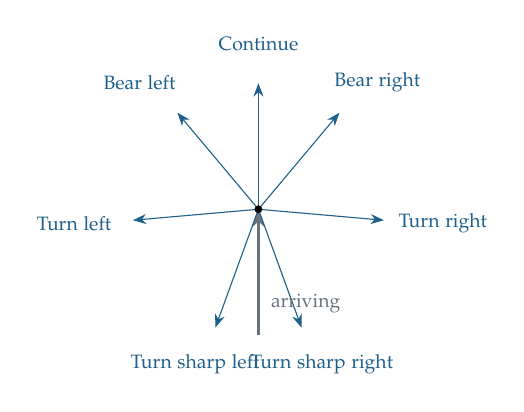
\begin{tikzpicture}[scale=1.0]
  \draw[color=cm, thick, -{Stealth}] (0,-1.6) -- (0,0);
  \foreach \a/\lab in {0/Continue, 40/Bear right, -40/Bear left, 95/Turn right,
      -95/Turn left, 160/Turn sharp right, -160/Turn sharp left} {
    \draw[accent, -{Stealth}] (0,0) -- ({1.6*sin(\a)},{1.6*cos(\a)});
    \node[font=\scriptsize, text=accent] at ({2.35*sin(\a)},{2.1*cos(\a)}) {\lab};
  }
  \fill (0,0) circle (0.05);
  \node[font=\scriptsize, text=cm] at (0.6,-1.2) {arriving};
\end{tikzpicture}
\end{center}

Less than $25^\circ$ either way is carrying straight on; up to $60^\circ$
is bearing left or right; up to $140^\circ$ is turning; more than that is
turning sharply, nearly back the way you came.

\begin{newfile}{directions.nex}
-- directions.nex: turning a route into instructions a person can follow.

intern Search
intern Helpers

-- One instruction: what to do, where, and how far into the route.
class Instruction
create
  make(words: String, at: Integer, metres, degrees: Real) do
    text := words
    node := at
    distance := metres
    turn := degrees
  end
feature
  -- What to do: "Turn left onto Mill Lane".
  once text: String
  -- The node where it happens.
  once node: Integer
  -- How far it is from the start of the route, in metres.
  once distance: Real
  -- How sharply the traveller turns there, in degrees: positive to the
  -- right, negative to the left, 0 for straight on.
  once turn: Real
end

-- The words for a turn of `angle` degrees (positive to the right).
function manoeuvre(angle: Real): String do
  let side: String := when angle > 0.0 then "right" else "left" end
  if angle.abs < 25.0 then
    result := "Continue"
  elseif angle.abs < 60.0 then
    result := "Bear " + side
  elseif angle.abs < 140.0 then
    result := "Turn " + side
  else
    result := "Turn sharp " + side
  end
end
\end{newfile}

Each instruction remembers how far into the route it is. The navigator
will need that, to say ``in 300 m''. It also keeps the turn's angle, so
that the live map can draw an arrow bending the right way.

\section{The instructions}

\begin{append}{directions.nex}
-- Instructions for following `path` to `destination`.
--
-- A route can have dozens of nodes, but a person needs to be told
-- something only where the road changes. So the route is cut into
-- stretches along one road each. The first instruction says which way to
-- set off; each later stretch starts with the turn onto its road; and the
-- last instruction says that the traveller has arrived.
function directions(g: Road_Graph, path: Array[Integer], destination: String): Array[Instruction]
require
  is_a_route: is_route(g, path)
do
  let pts: Array[Point] := g.island.points_of(path)
  if path.length = 1 then
    result.add(create Instruction.make("You are at " + destination, path.get(0), 0.0, 0.0))
  else
    let travelled: Real := 0.0
    let previous: ?Edge := nil
    from
      let i: Integer := 0
    until
      i = path.length - 1
    do
      if ?g.edge_between(path.get(i), path.get(i + 1)) as e then
        if ?previous as before then
          if e.road.name /= before.road.name then
            let angle: Real := turn_angle(bearing(pts.get(i - 1), pts.get(i)),
              bearing(pts.get(i), pts.get(i + 1)))
            result.add(create Instruction.make(manoeuvre(angle) + " onto " + e.road.name,
              path.get(i), travelled, angle))
          end
        else
          result.add(create Instruction.make("Head "
            + compass_name(bearing(pts.get(0), pts.get(1))) + " on " + e.road.name,
            path.get(0), 0.0, 0.0))
        end
        travelled := travelled + e.length
        previous := e
      end
      i := i + 1
    end
    result.add(create Instruction.make("Arrive at " + destination,
      path.get(path.length - 1), travelled, 0.0))
  end
ensure
  starts_at_start: result.get(0).distance = 0.0
  ends_at_end: (result.get(result.length - 1).distance
    - route_cost(g, path, by_distance())).abs < 0.001
end
\end{append}

\code{previous} is the edge before the current one, or \code{nil} for the
very first edge. \code{?previous as before} is Nex's \emph{object test}:
it is true when \code{previous} is not \code{nil}, and inside the
\code{if} it names the edge \code{before}, with the type \code{Edge}
instead of \code{?Edge}, so that we can use its road. On the first edge
there is no edge before, so that is where we say which way to set off.

The postcondition checks that the distances add up: the last instruction
is exactly as far into the route as the route is long.

Real navigators say a good deal more than ours: ``keep left'' where a road
forks, ``take the second exit'' at a roundabout, ``turn right after the
church'' when there is a landmark, and they warn about turns where the road
keeps its name but the route leaves it. They all start from the same idea:
find the places where something changes, and describe the change.

\section{A route planner}

Now everything comes together in a program. It takes two place names, and
a few options, from the command line, plans a route, and prints its
instructions, with the distance of each stretch.

\begin{newfile}{route.nex}
-- route.nex: directions from one place to another, printed.
--
--   nex route.nex                              -- list the places
--   nex route.nex "The Harbour" Lighthouse     -- the quickest way by car
--   nex route.nex harbour lighthouse --walk    -- on foot
--   nex route.nex harbour lighthouse --shortest
--   nex route.nex harbour lighthouse --algorithm dijkstra   (or bfs, astar)
--
-- A place can be given by part of its name: "mill" is "Old Mill".

intern Directions
intern Helpers

function main() do
  let args: Array[String] := program.arguments
  let names: Array[String] := []
  let mode: Mode := Mode.Driving
  let shortest: Boolean := false
  let algorithm: String := "astar"
  let map_file: String := "kestrel_island.map"
  from
    let i: Integer := 0
  until
    i >= args.length
  do
    let arg: String := args.get(i)
    if arg = "--walk" then
      mode := Mode.Walking
    elseif arg = "--shortest" then
      shortest := true
    elseif arg = "--algorithm" and i + 1 < args.length then
      algorithm := args.get(i + 1)
      i := i + 1
    elseif arg = "--map" and i + 1 < args.length then
      map_file := args.get(i + 1)
      i := i + 1
    else
      names.add(arg)
    end
    i := i + 1
  end
\end{newfile}

\code{program.arguments} gives the words typed after the
program's name. Options start with \code{--}; anything else is a place
name. Next, with the map loaded, either explain how to use the program,
or plan the route:

\begin{continued}{route.nex}
  let island: Island_Map := create Island_Map.load(user_path(map_file))
  if names.length /= 2 then
    console.print_line("usage: nex route.nex FROM TO [--walk] [--shortest] [--algorithm bfs|dijkstra|astar]")
    console.print_line("")
    console.print_line("Places on " + island.name + ":")
    across island.places as p do
      console.print_line("  " + p.name)
    end
  elseif ?island.find_place(names.get(0)) as start
      and ?island.find_place(names.get(1)) as finish then
    let g: Road_Graph := create Road_Graph.build(island, mode)
    let source: Integer := g.nearest_node(island.point(start.node_id))
    let target: Integer := g.nearest_node(island.point(finish.node_id))
    let found: Search_Result := find_route(g, source, target, algorithm, shortest)
    if found.found() then
      print_route(g, found, start.name, finish.name)
    else
      console.print_line("There is no way from " + start.name + " to " + finish.name + ".")
    end
  else
    console.print_line("I don't know one of those places. Run nex route.nex to list them.")
  end
end
\end{continued}

The instructions are printed numbered, each with the length of its stretch:
the distance from it to the next instruction.

\begin{continued}{route.nex}
function print_route(g: Road_Graph, found: Search_Result, from_name, to_name: String) do
  let how: String := when g.mode = Mode.Walking then "Walking" else "Driving" end
  console.print_line(how + " from " + from_name + " to " + to_name + ": "
    + distance_text(route_cost(g, found.path, by_distance())) + ", about "
    + duration_text(route_cost(g, found.path, by_time())) + ".")
  console.print_line(found.algorithm + " explored " + found.explored.length.to_string
    + " of the " + g.nodes.length.to_string + " nodes.")
  console.print_line("")
  let steps: Array[Instruction] := directions(g, found.path, to_name)
  from
    let i: Integer := 0
  until
    i = steps.length
  do
    let step: Instruction := steps.get(i)
    let line: String := (i + 1).to_string.pad_start(" ", 3) + ". " + step.text
    if i + 1 < steps.length then
      line := line.pad_end(" ", 42)
        + distance_text(steps.get(i + 1).distance - step.distance).pad_start(" ", 8)
    end
    console.print_line(line)
    i := i + 1
  end
end

main()
\end{continued}

\section{Planning some trips}

With no places, the program lists them:

\runoutput{route.nex}{route_places}

From the beach to the lighthouse, by car, the quickest way and the
shortest:

\runoutput{route.nex "beach car park" lighthouse}{route_beach}
\runoutput{route.nex beach lighthouse --shortest}{route_beach_shortest}

From Market Square to the harbour, a few hundred metres, by car and on
foot. The one-way streets send the car east, then south down Chapel
Street, and back west along the quay; the walker goes straight down
Harbour Street:

\runoutput{route.nex market harbour}{route_market_drive}
\runoutput{route.nex market harbour --walk}{route_market_walk}

And from Kestrel Peak, in the middle of Hollow Wood, to the lighthouse. A
car must take the track out of the wood and go round by the Coast Road;
on foot, the paths over the hill and along the cliffs are much shorter:

\runoutput{route.nex peak lighthouse}{route_peak_drive}
\runoutput{route.nex peak lighthouse --walk}{route_peak_walk}

\section{Checking the directions}

Two more checks: that the directions start and end the way they should, and
that the one-way streets really do send drivers round by Chapel Street
while walkers go the short way.

\begin{addbefore}{checks.nex}{before main}{function main() do}
function check_directions(c: Checker, m: Island_Map, driving, walking: Road_Graph) do
  if ?m.find_place("market") as a and ?m.find_place("harbour") as b then
    let drive: Search_Result := dijkstra(driving, node_of(driving, a), node_of(driving, b), by_time())
    let steps: Array[Instruction] := directions(driving, drive.path, b.name)
    c.check("directions start by setting off", steps.get(0).text.starts_with("Head "))
    c.check("directions end by arriving", steps.get(steps.length - 1).text = "Arrive at The Harbour")
    let detour: Boolean := false
    across steps as step do
      if step.text = "Turn right onto Chapel Street" then
        detour := true
      end
    end
    c.check("one-way streets send drivers round by Chapel Street", detour)
    let walk: Search_Result := dijkstra(walking, node_of(walking, a), node_of(walking, b), by_time())
    c.check("walkers go the short way", route_cost(walking, walk.path, by_distance())
      < route_cost(driving, drive.path, by_distance()))
  end
  c.check("manoeuvres", manoeuvre(5.0) = "Continue" and manoeuvre(-40.0) = "Bear left"
    and manoeuvre(90.0) = "Turn right" and manoeuvre(-170.0) = "Turn sharp left")
end
\end{addbefore}

\begin{tightaddbefore}{checks.nex}{to main, before c.summary()}{  c.summary()}
  check_directions(c, m, driving, walking)
\end{tightaddbefore}

The checks now use \code{directions.nex}, so we intern it at the top of the
file. (\code{directions.nex} interns \code{search.nex} itself, so the
second \code{intern} is no longer needed, but interning a file twice is
harmless.)

\begin{tightaddbefore}{checks.nex}{at the top}{intern Search}
intern Directions
\end{tightaddbefore}

% ===========================================================================
\chapter{Following the traveller}\label{ch:following}

Printed directions are planned once and read once. A navigator is
different: it rides along. About once a second, the GPS gives it a new
position, a \emph{fix}, and it must work out:

\begin{itemize}[nosep]
  \item how far along the route the traveller has got;
  \item what the next instruction is, and how far away;
  \item how far there is still to go, and how long it will take;
  \item and whether the traveller is still on the route at all.
\end{itemize}

\section{Noisy fixes}

A GPS fix is never exactly right. Out in the open, a phone is usually
within about five metres of the truth; between tall buildings, where the
satellites' signals bounce off walls, it can be out by fifty. A fix taken
while driving down the middle of a road might put the car in a garden.

So a navigator never takes a fix at face value. It assumes the traveller
is on the road, most likely on the route it planned, and moves each fix to
the nearest point of the route. This is called \emph{map matching}. The
distance between the fix and that point, the \emph{offset}, says how well
they match: a few metres is noise, but fifty metres, again and again, means
the traveller is somewhere else.

\section{The route as a line}

For following a route, we want it as a line on the map, with a ruler
along it: for any point of the route, how far along it is. We store, for
each node of the route, the distance from the start of the route to that
node, and the time it takes to get there.

\begin{center}
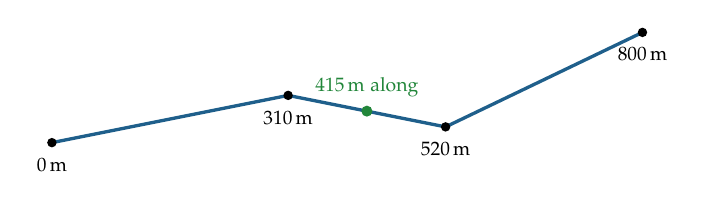
\begin{tikzpicture}[x=1cm, y=1cm]
  \draw[accent, very thick] (0,0) -- (3,0.6) -- (5,0.2) -- (7.5,1.4);
  \foreach \p/\d in {(0,0)/0, (3,0.6)/310, (5,0.2)/520, (7.5,1.4)/800}
    \fill \p circle (0.06) node[below=2pt, font=\scriptsize] {\d\,m};
  \fill[st] (4,0.4) circle (0.07);
  \node[font=\scriptsize, text=st, above] at (4,0.45) {415\,m along};
\end{tikzpicture}
\end{center}

A point $d$ metres along the route is on the segment whose start is at
most $d$ along and whose end is more than $d$ along. Within that segment,
it is a fraction of the way from start to end, and so is its time: the
time at the start of the segment, plus the same fraction of the segment's
time.

\begin{newfile}{navigation.nex}
-- navigation.nex: following a route as the traveller moves. Knowing how
-- far along the route they are, what to tell them next, and when they
-- have left the route.

intern Directions
intern Helpers

-- Where a position lies relative to a line: the nearest point of the
-- line, how far along the line that point is, and how far the position
-- is from it.
class Line_Match
create
  make(p: Point, d, off: Real) do
    point := p
    along := d
    offset := off
  end
feature
  once point: Point
  -- Metres from the start of the line.
  once along: Real
  -- Metres from the line.
  once offset: Real
end

-- A route as a line on the map, measured along its length.
class Route_Line
create
  make(g: Road_Graph, path: Array[Integer])
  require
    is_a_route: is_route(g, path)
  do
    nodes := path
    points := g.island.points_of(path)
    along := [0.0]
    times := [0.0]
    from
      let i: Integer := 1
    until
      i = path.length
    do
      if ?g.edge_between(path.get(i - 1), path.get(i)) as e then
        along.add(along.get(i - 1) + e.length)
        times.add(times.get(i - 1) + e.seconds)
      end
      i := i + 1
    end
  end
feature
  nodes: Array[Integer]
  points: Array[Point]
  -- How far along the route each node is, in metres...
  along: Array[Real]
  -- ...and how long it takes to get there, in seconds.
  times: Array[Real]

  length(): Real do
    result := along.get(along.length - 1)
  end

  duration(): Real do
    result := times.get(times.length - 1)
  end
\end{newfile}

Now the questions about a point $d$ metres along: which segment it is on,
where it is, which way the route is heading there, and how long it takes to
get there. A route with only one node, from a place to itself, has no
segments at all, and each query handles that first.

\begin{continued}{navigation.nex}
  -- The segment that the point `d` metres along the route is on: i for
  -- the segment from node i to node i + 1.
  segment_at(d: Real): Integer do
    result := 0
    from
    until
      result >= points.length - 2 or along.get(result + 1) > d
    do
      result := result + 1
    end
  ensure
    valid_segment: result >= 0 and (result < points.length - 1 or points.length = 1)
  end

  -- The point `d` metres along the route.
  point_at(d: Real): Point do
    if points.length = 1 then
      result := points.get(0)
    else
      let i: Integer := segment_at(d)
      result := points.get(i) + (points.get(i + 1) - points.get(i)) * fraction(i, d)
    end
  end

  -- The direction of travel `d` metres along the route.
  heading_at(d: Real): Real do
    if points.length = 1 then
      result := 0.0
    else
      let i: Integer := segment_at(d)
      result := bearing(points.get(i), points.get(i + 1))
    end
  end

  -- How long it takes to travel the first `d` metres of the route.
  time_at(d: Real): Real do
    if points.length = 1 then
      result := 0.0
    else
      let i: Integer := segment_at(d)
      result := times.get(i) + (times.get(i + 1) - times.get(i)) * fraction(i, d)
    end
  end
\end{continued}

For drawing, the live map will show the part of the route already travelled
in grey and the rest in blue, so the line can be cut in two at any point:

\begin{continued}{navigation.nex}
  -- The route from `d` metres on (or up to `d` metres, if not `after`),
  -- as a line, for drawing.
  part(d: Real, after: Boolean): Array[Point] do
    let i: Integer := segment_at(d)
    if after then
      result.add(point_at(d))
      result := result.concat(points.drop(i + 1))
    else
      result := points.take(i + 1)
      result.add(point_at(d))
    end
  end
\end{continued}

\section{Map matching}

To match a fix to the route, we use \code{closest_point_on_segment}, from
Chapter~\ref{ch:geometry}, to find the closest point of every segment, and
keep the nearest. How far along the route is it? As far as the start of its
segment, plus its distance from that start.

There is a catch. Routes can double back, or run close beside themselves:
out along a lane and back along the same lane, or down one street and up
the next. The nearest point of the whole route might be on a part the
traveller won't reach for minutes, and if we believed it, the navigator
would suddenly announce the instructions for the way back. So we search
only a \emph{window} of the route, between \code{low} and \code{high}
metres along it, around where the traveller was a moment ago. Real
navigators do the same, and more: they also use the direction and speed of
travel, and they weigh up several candidate roads over several fixes before
deciding.

\begin{continued}{navigation.nex}
  -- Where p is relative to the stretch of the route between `low` and
  -- `high` metres along it.
  locate(p: Point, low, high: Real): Line_Match do
    result := create Line_Match.make(points.get(0), 0.0, p.distance_to(points.get(0)))
    from
      let i: Integer := 0
    until
      i >= points.length - 1
    do
      if along.get(i + 1) >= low and along.get(i) <= high then
        let a: Point := points.get(i)
        let c: Point := closest_point_on_segment(p, a, points.get(i + 1))
        let off: Real := p.distance_to(c)
        if off < result.offset then
          result := create Line_Match.make(c, along.get(i) + a.distance_to(c), off)
        end
      end
      i := i + 1
    end
  end

private feature
  -- How far through segment i the point d metres along the route is,
  -- from 0 at its start to 1 at its end.
  fraction(i: Integer, d: Real): Real do
    let seg: Real := along.get(i + 1) - along.get(i)
    if seg > 0.0 then
      result := ((d - along.get(i)) / seg).clamp(0.0, 1.0)
    end
  end
end
\end{continued}

\section{The navigator}

The navigator holds the route and its instructions, and the one number
that matters most: its \emph{progress}, how far along the route the
traveller is. It also keeps the graph and the search algorithm, which it
will need in the next chapter, to plan a new route when the traveller goes
astray.

\begin{append}{navigation.nex}
-- The navigator: it knows the route, takes in GPS fixes, and says what to
-- do next.
class Navigator
create
  make(g: Road_Graph, path: Array[Integer], place: String, how: String)
  require
    is_a_route: is_route(g, path)
  do
    graph := g
    destination := place
    algorithm := how
    progress := 0.0
    misses := 0
    reroutes := 0
    route := create Route_Line.make(g, path)
    instructions := directions(g, path, place)
    last_fix := route.point_at(0.0)
  end
feature
  graph: Road_Graph
  -- The destination's name, and the algorithm used to plan routes to it.
  destination: String
  algorithm: String
  route: Route_Line
  instructions: Array[Instruction]
  -- How far along the route the traveller is, in metres.
  progress: Real
  -- How many fixes in a row have been too far from the route.
  misses: Integer
  -- How many times the route has been planned again.
  reroutes: Integer
  last_fix: Point
\end{append}

Each fix is matched to the route, looking from 40 metres behind the last
progress to 250 metres ahead of it. Driving at 60\,km/h, a car covers about
17 metres a second, so 250 metres is plenty of room ahead.

If the fix matches within 25 metres, the traveller is on the route, and
the progress moves up to where the fix matched. It never goes backwards:
the noise in the fixes makes the matched point jitter back and forth by a
few metres, and a navigator whose ``in 200 m'' becomes ``in 205 m'' looks
broken. The postcondition holds the navigator to that, with \code{old}:
in an \code{ensure}, \code{old progress} is the value \code{progress} had
when the routine was called.

If the fix is further away, it is a \emph{miss}. One miss might be a bad
fix. Three in a row, and the traveller has left the route.

\begin{continued}{navigation.nex}
  -- A fix further than this from the route doesn't count as on it...
  TOLERANCE = 25.0
  -- ...and this many of those in a row mean the traveller has left it.
  PATIENCE = 3
  -- How far back and ahead of the last known progress to look for the
  -- traveller on the route.
  LOOK_BACK = 40.0
  LOOK_AHEAD = 250.0

  -- Take in a new GPS fix.
  --
  -- GPS fixes are a few metres off, so the navigator moves each one to the
  -- nearest point of the route: this is called map matching. It looks
  -- only near where the traveller was a moment ago. A route can pass the
  -- same place twice, or run close to itself, and the nearest point of the
  -- whole route might be on a part the traveller has not reached yet.
  update(fix: Point) do
    last_fix := fix
    let m: Line_Match := route.locate(fix, (progress - LOOK_BACK).max(0.0),
      progress + LOOK_AHEAD)
    if m.offset <= TOLERANCE then
      progress := progress.max(m.along)
      misses := 0
    else
      misses := misses + 1
    end
  ensure
    no_going_back: progress >= old progress
  end

  is_off_route(): Boolean do
    result := misses >= PATIENCE
  end

  has_arrived(): Boolean do
    result := progress >= route.length() - 15.0
  end
\end{continued}

\section{What to say}

The next instruction is the first one further along the route than the
traveller. What to say about it depends on how far away it is: far off,
``In 300 m, turn left onto Mill Lane''; close by, ``Turn left onto Mill
Lane now''. And the time still to go is the route's whole duration, less
the time it takes to get to where the traveller is.

\begin{continued}{navigation.nex}
  -- The next instruction the traveller has not reached yet.
  next_instruction(): Instruction do
    result := instructions.get(instructions.length - 1)
    let found: Boolean := false
    across instructions as step do
      if not found and step.distance > progress + 1.0 then
        result := step
        found := true
      end
    end
  end

  -- What to say now: "In 300 m, turn left onto Mill Lane".
  prompt(): String do
    let next: Instruction := next_instruction()
    let d: Real := next.distance - progress
    if has_arrived() then
      result := "You have arrived at " + destination
    elseif d < 30.0 then
      result := next.text + " now"
    else
      result := "In " + distance_text(d) + ", " + lowercase_first(next.text)
    end
  end

  remaining_distance(): Real do
    result := (route.length() - progress).max(0.0)
  end

  remaining_time(): Real do
    result := (route.duration() - route.time_at(progress)).max(0.0)
  end
end

-- s with its first letter in lower case: "Turn left" -> "turn left".
function lowercase_first(s: String): String do
  if s.length = 0 then
    result := s
  else
    result := s.substring(0, 1).to_lower() + s.substring(1, s.length)
  end
end
\end{continued}

The remaining time comes from the route's own times, edge by edge, so it
knows that the rest of the trip is on a slow track or a fast main road.
Real navigators improve on this all the time, with the traveller's actual
speed and with live traffic.

\section{A pretend drive}

We don't have a traveller yet; the next chapter makes one. For now we can
pretend: take points along the route every 100 metres, push each one a few
metres off to the side, the way a GPS would, and give them to the
navigator. \code{direction(heading + 90.0)} is an arrow pointing square to
the right of the route, so adding six metres of it moves a point six metres
to the right.

\begin{tryit}{try_navigator.nex}
intern Navigation

let island: Island_Map := create Island_Map.load(user_path("kestrel_island.map"))
let g: Road_Graph := create Road_Graph.build(island, Mode.Driving)
if ?island.find_place("harbour") as a and ?island.find_place("lighthouse") as b then
  let found: Search_Result := find_route(g, g.nearest_node(island.point(a.node_id)),
    g.nearest_node(island.point(b.node_id)), "astar", false)
  let nav: Navigator := create Navigator.make(g, found.path, b.name, "astar")
  let line: Route_Line := nav.route
  console.print_line("route: " + distance_text(line.length()) + ", " + duration_text(line.duration()))
  let d: Real := 0.0
  let side: Real := 6.0
  from
  until
    d > line.length() + 100.0
  do
    let fix: Point := line.point_at(d) + direction(line.heading_at(d) + 90.0) * side
    nav.update(fix)
    if (d / 100.0).round % 5 = 0 or nav.has_arrived() then
      console.print_line(nav.progress.format(0).pad_start(" ", 5) + " m  " + nav.prompt().pad_end(" ", 42)
        + distance_text(nav.remaining_distance()) + ", " + duration_text(nav.remaining_time()))
    end
    d := d + 100.0
    side := -side
  end

  -- Another drive, which turns off the route 600 m from the start.
  let lost: Navigator := create Navigator.make(g, found.path, b.name, "astar")
  from
    d := 0.0
  until
    d > 600.0
  do
    lost.update(line.point_at(d))
    d := d + 100.0
  end
  repeat 3 do
    lost.update(line.point_at(600.0) + direction(line.heading_at(600.0) + 90.0) * 60.0)
    console.print_line("a fix 60 m from the route: " + lost.misses.to_string + " in a row, off the route: "
      + lost.is_off_route().to_string)
  end
end
\end{tryit}
\tryoutput{try_navigator}

Every fix was six metres to the left or right of the road, and every one
was matched back onto it. The prompts count down to the next change of
road, and the time left comes down as the distance does.

On the second drive, after 600 metres the fixes are suddenly 60 metres
from the route. One or two such fixes could be bad readings; three in a
row mean the traveller has left the route. What then? That is the next
chapter.

% ===========================================================================
\chapter{Wrong turns}\label{ch:wrongturn}

Every driver misses a turn now and then. A navigator can't stop them; it
can only notice, quickly, and work out a new way from wherever they have
ended up. ``Recalculating\ldots'' This chapter teaches the navigator to do
that, and then builds a pretend traveller, with a pretend GPS, to try it
out on.

\section{Where is the traveller now?}

When the traveller has left the route, the navigator's progress along it
means nothing any more. All it has is the last GPS fix. So, as before, it
assumes the traveller is on a road, but this time any road of the map, not
just the route: it finds the edge nearest to the fix.

Each two-way stretch of road is two edges, one each way, at exactly the
same distance from the fix. Which way is the traveller going? Away from
the route, most likely, since that is how they come to be off it. So of the
two, we take the edge whose end is further from the point where the
traveller left the route.

\begin{append}{navigation.nex}
-- The edge of g nearest p, going away from `behind`: of the two
-- directions along the nearest stretch of road, the one whose end is
-- further from `behind`.
function rejoin(g: Road_Graph, p: Point, behind: Point): Edge
require
  has_edges: g.edge_count > 0
do
  let all: Array[Edge] := []
  across g.nodes as id do
    all := all.concat(g.edges_from(id))
  end
  result := all.get(0)
  let best: Real := distance_to_segment(p, g.island.point(result.source),
    g.island.point(result.target))
  across all as e do
    let a: Point := g.island.point(e.source)
    let b: Point := g.island.point(e.target)
    let d: Real := distance_to_segment(p, a, b)
    let better: Boolean := d < best - 0.5
    if not better and (d - best).abs <= 0.5 then
      -- The same stretch of road the other way: keep the direction that
      -- leads away from `behind`.
      better := b.distance_to(behind) > g.island.point(result.target).distance_to(behind)
    end
    if better then
      best := d
      result := e
    end
  end
end
\end{append}

Two distances within half a metre of each other count as a tie, since two
edges along the same stretch of road should be exactly equal, but rounding
might make them differ in the last decimal place.

\section{Planning again}

The new route starts with the edge the traveller is on, and continues with
the best way from the end of that edge to the destination, planned with
the same algorithm as before. The traveller is already part of the way
along the first edge, so the progress starts there: the distance from the
edge's start to the point of the edge nearest the fix.

\begin{addbefore}{navigation.nex}{to Navigator, before is_off_route}{  is_off_route(): Boolean do}
  -- Plan a new route from where the traveller is now.
  --
  -- The navigator knows only the GPS fixes. The traveller is on the road
  -- nearest the last fix, heading away from where they left the route. So
  -- the new route starts with that stretch of road, and continues with
  -- the best way from the end of it to the destination.
  reroute() do
    let left_at: Point := route.point_at(progress)
    let e: Edge := rejoin(graph, last_fix, left_at)
    let goal: Integer := route.nodes.get(route.nodes.length - 1)
    let rest: Search_Result := find_route(graph, e.target, goal, algorithm, false)
    if rest.found() then
      let path: Array[Integer] := [e.source].concat(rest.path)
      route := create Route_Line.make(graph, path)
      instructions := directions(graph, path, destination)
      let a: Point := graph.island.point(e.source)
      progress := a.distance_to(closest_point_on_segment(last_fix, a,
        graph.island.point(e.target)))
      misses := 0
      reroutes := reroutes + 1
    end
  end
\end{addbefore}

The new route may well begin by turning round: if the traveller has just
gone the wrong way down a long road with no turnings, the quickest way back
may be a U-turn. The directions will say so: ``Turn sharp left''.

\section{A pretend traveller}

To watch all this happen, we need someone to navigate. Our traveller
moves along a path of nodes, at the speed of each road: an edge of 100
metres that takes 12 seconds to drive is covered at $100/12$ metres per
second. The traveller knows where it really is: on the edge from
\code{path[leg]} to \code{path[leg + 1]}, \code{offset} metres along it.

\begin{newfile}{simulation.nex}
-- simulation.nex: a pretend traveller with a pretend GPS, so that the
-- navigator has someone to guide.

intern Navigation
intern Rng

-- The traveller, moving along a path of nodes at the speed of each road.
-- Usually the path is the navigator's route, but a traveller can take a
-- wrong turn.
class Traveller
create
  make(g: Road_Graph, nodes: Array[Integer])
  require
    is_a_route: is_route(g, nodes)
    can_move: nodes.length >= 2
  do
    graph := g
    path := nodes
    leg := 0
    offset := 0.0
    wrong_turn_pending := false
  end
feature
  graph: Road_Graph
  -- The nodes the traveller means to pass through.
  path: Array[Integer]
  -- The traveller is `offset` metres along the edge from path[leg] to
  -- path[leg + 1].
  leg: Integer
  offset: Real
  -- Set to make the traveller go the wrong way at the next junction.
  wrong_turn_pending: Boolean

  has_arrived(): Boolean do
    result := leg >= path.length - 1
  end

  -- The edge the traveller is on.
  edge(): Edge
  require
    on_the_way: not has_arrived()
  do
    if ?graph.edge_between(path.get(leg), path.get(leg + 1)) as e then
      result := e
    else
      raise "the traveller's path has a step that is not an edge"
    end
  end

  -- Where the traveller really is.
  position(): Point do
    if has_arrived() then
      result := graph.island.point(path.get(path.length - 1))
    else
      let a: Point := graph.island.point(path.get(leg))
      let b: Point := graph.island.point(path.get(leg + 1))
      result := a + (b - a) * (offset / a.distance_to(b))
    end
  end

  -- Which way the traveller is facing, as a compass bearing.
  heading(): Real do
    if path.length < 2 then
      result := 0.0
    else
      let i: Integer := leg.min(path.length - 2)
      result := bearing(graph.island.point(path.get(i)), graph.island.point(path.get(i + 1)))
    end
  end

  -- Go the wrong way at the next junction.
  take_wrong_turn() do
    wrong_turn_pending := true
  end
\end{newfile}

Moving on by some number of seconds means covering the rest of the current
edge, if there is time, then the next edge, and so on, until the time is
used up or the traveller arrives. Each time the traveller reaches a node,
if a wrong turn is due, it takes it there.

\begin{continued}{simulation.nex}
  -- Move on by `seconds` of travel.
  advance(seconds: Real)
  require
    non_negative: seconds >= 0.0
  do
    let left: Real := seconds
    from
    until
      left <= 0.0 or has_arrived()
    do
      let e: Edge := edge()
      let speed: Real := e.length / e.seconds
      let to_go: Real := (e.length - offset) / speed
      if left < to_go then
        offset := offset + left * speed
        left := 0.0
      else
        left := left - to_go
        offset := 0.0
        leg := leg + 1
        if wrong_turn_pending and not has_arrived() then
          go_wrong()
        end
      end
    end
  end
\end{continued}

When the navigator plans a new route, the traveller takes it. The new route
starts with the edge the navigator believes the traveller is on; if that is
the edge the traveller really is on, the traveller simply swaps its path
for the new one. If the traveller has already reached the end of that edge,
the new route starts where it is about to arrive, which works too. If
neither, the navigator has guessed wrong, and the traveller carries on
regardless. The navigator will soon find it off the new route as well, and
try again.

\begin{continued}{simulation.nex}
  -- Take the navigator's new route, which starts on the traveller's edge
  -- or at the node the traveller is about to reach.
  follow(nodes: Array[Integer]) do
    if has_arrived() then
      if nodes.get(0) = path.get(path.length - 1) and nodes.length >= 2 then
        path := nodes
        leg := 0
        offset := 0.0
      end
    elseif nodes.length >= 2 and nodes.get(0) = path.get(leg)
        and nodes.get(1) = path.get(leg + 1) then
      path := nodes
      leg := 0
    elseif nodes.get(0) = path.get(leg + 1) then
      path := [path.get(leg)].concat(nodes)
      leg := 0
    end
  end
\end{continued}

A wrong turn happens at a junction: a node with some way out other than
the planned one and the one the traveller came from. Most nodes of a route
are not junctions, just points along a road, so a wrong turn that is due
waits for the next real junction. There, the traveller takes whichever
other road turns least, the classic mistake of going straight on when the
route turns, and then simply keeps going as straight as it can, for a
dozen edges, wherever that leads.

\begin{continued}{simulation.nex}
private feature
  -- At path[leg], turn off the planned way onto another road, and keep
  -- going straight on, wherever that leads.
  go_wrong() do
    let here: Integer := path.get(leg)
    let came_from: Integer := path.get(leg - 1)
    let planned: Integer := path.get(leg + 1)
    let options: Array[Edge] := []
    across graph.edges_from(here) as e do
      if e.target /= came_from and e.target /= planned then
        options.add(e)
      end
    end
    if not options.is_empty then
      let wrong: Edge := straightest(came_from, here, options)
      let detour: Array[Integer] := [wrong.target]
      let previous: Integer := here
      repeat 12 do
        let at: Integer := detour.get(detour.length - 1)
        let onward: Array[Edge] := []
        across graph.edges_from(at) as e do
          if e.target /= previous then
            onward.add(e)
          end
        end
        if not onward.is_empty then
          detour.add(straightest(previous, at, onward).target)
          previous := at
        end
      end
      path := path.take(leg + 1).concat(detour)
      wrong_turn_pending := false
    end
  end

  -- Of `options`, the edges leaving `at`, the one that turns least for a
  -- traveller arriving from `before`.
  straightest(before, at: Integer, options: Array[Edge]): Edge
  require
    has_options: not options.is_empty
  do
    let island: Island_Map := graph.island
    let heading_in: Real := bearing(island.point(before), island.point(at))
    result := options.get(0)
    across options as e do
      let turn: Real := turn_angle(heading_in, bearing(island.point(at), island.point(e.target))).abs
      let best: Real := turn_angle(heading_in, bearing(island.point(at),
        island.point(result.target))).abs
      if turn < best then
        result := e
      end
    end
  end
end
\end{continued}

\section{A pretend GPS}

A real GPS fix is off by a few metres, in a random direction, by a random
amount: usually a little, occasionally more. Errors like that follow the
\emph{normal distribution}, the bell curve. To make them, we need random
numbers, and to be able to repeat a run exactly (so that the pictures in
this tutorial come out the same every time), the random numbers must come
from a generator we can \emph{seed}: start from a chosen number, and get
the same sequence every time.

\begin{newfile}{rng.nex}
-- rng.nex: a small random number generator that can be seeded, for the
-- simulated GPS. With a seed, the "random" numbers are the same on every
-- run, so a simulated trip can be repeated exactly.
--
-- This is the Park-Miller "minimal standard" generator:
--     state := state * 48271 mod (2^31 - 1)

class Rng
create
  make(seed: Integer) do
    state := 1 + seed.abs % (MODULUS - 1)
  end
feature
  MODULUS = 2147483647
  MULTIPLIER = 48271

  state: Integer

  -- A real number spread evenly over the open interval (0, 1).
  uniform(): Real
  do
    state := (state * MULTIPLIER) % MODULUS
    result := state.to_real / MODULUS.to_real
  ensure
    open_interval: result > 0.0 and result < 1.0
  end

  -- A number from the standard normal ("bell curve") distribution, with
  -- mean 0 and standard deviation 1, by the Box-Muller transform.
  gauss(): Real do
    let radius: Real := (-2.0 * uniform().log).sqrt
    let angle: Real := 2.0 * Real.PI * uniform()
    result := radius * angle.cos
  end
invariant
  state_in_range: state >= 1 and state < MODULUS
end
\end{newfile}

The generator multiplies its state by 48,271 and keeps the remainder after
dividing by $2^{31} - 1$, a prime number. The result jumps about so
thoroughly that it looks random, and dividing by the modulus gives a number
between 0 and 1.

The \emph{Box--Muller transform} turns two such evenly spread numbers,
$u_1$ and $u_2$, into one from the bell curve: $\sqrt{-2\ln u_1}
\cos(2\pi u_2)$. It is a neat piece of mathematics: picking a random angle,
$2\pi u_2$, and a random distance, $\sqrt{-2\ln u_1}$, gives a point whose
$x$ and $y$ both follow the bell curve. We use just the $x$.

A fix is then the true position plus a normal error in each direction,
four metres on average:

\begin{append}{simulation.nex}
-- A pretend GPS receiver. Every fix is the true position plus a random
-- error of a few metres, the way a real one is.
class Gps
create
  make(seed: Integer, metres: Real) do
    rng := create Rng.make(seed)
    error := metres
  end
feature
  rng: Rng
  -- The typical size of the error, in metres (its standard deviation).
  error: Real

  fix(truth: Point): Point do
    result := truth + create Point.make(rng.gauss() * error, rng.gauss() * error)
  end
end
\end{append}

\section{A trip}

Finally, a trip puts the traveller, the GPS and the navigator together, with
a clock. As the clock moves on, the traveller moves, and once a second the
GPS takes a fix and gives it to the navigator. If the navigator finds the
traveller off the route, it plans a new one, and the traveller takes it.

Notice how little the navigator is told. It never asks the traveller where
it is: it gets only fixes, with their errors, exactly as a real navigator
gets only what the GPS chip says.

\begin{append}{simulation.nex}
-- A trip: a traveller, their GPS, and the navigator guiding them, with
-- the clock that moves them all on together.
class Trip
create
  make(g: Road_Graph, path: Array[Integer], destination, algorithm: String, seed: Integer)
  require
    is_a_route: is_route(g, path)
    can_move: path.length >= 2
  do
    traveller := create Traveller.make(g, path)
    gps := create Gps.make(seed, 4.0)
    navigator := create Navigator.make(g, path, destination, algorithm)
    clock := 0.0
    next_fix := 0.0
    fix := traveller.position()
  end
feature
  traveller: Traveller
  gps: Gps
  navigator: Navigator
  -- Seconds since the trip began...
  clock: Real
  -- ...and when the GPS gives its next fix (once a second).
  next_fix: Real
  -- The latest fix.
  fix: Point

  -- Move the trip on by `seconds`.
  advance(seconds: Real) do
    let stop: Real := clock + seconds
    from
    until
      next_fix > stop
    do
      traveller.advance(next_fix - clock)
      clock := next_fix
      fix := gps.fix(traveller.position())
      navigator.update(fix)
      if navigator.is_off_route() then
        navigator.reroute()
        traveller.follow(navigator.route.nodes)
      end
      next_fix := next_fix + 1.0
    end
    traveller.advance(stop - clock)
    clock := stop
  end

  is_over(): Boolean do
    result := traveller.has_arrived() and navigator.has_arrived()
  end
end
\end{append}

\code{advance} can be asked to move on by any amount of time, a fraction of
a second or a minute, and it still takes a fix at every whole second in
between. The live map will move it on by whatever time has passed since
the last frame it drew.

\section{Taking a wrong turn}

This script drives from the harbour to the lighthouse. Forty seconds in,
it tells the traveller to take a wrong turn, and it prints what the
navigator says along the way: the prompt whenever the next instruction
changes, and every thirty seconds in between.

\begin{tryit}{try_trip.nex}
intern Simulation

let island: Island_Map := create Island_Map.load(user_path("kestrel_island.map"))
let g: Road_Graph := create Road_Graph.build(island, Mode.Driving)
if ?island.find_place("harbour") as a and ?island.find_place("lighthouse") as b then
  let found: Search_Result := find_route(g, g.nearest_node(island.point(a.node_id)),
    g.nearest_node(island.point(b.node_id)), "astar", false)
  let trip: Trip := create Trip.make(g, found.path, b.name, "astar", 7)
  console.print_line("   0 s  " + trip.navigator.prompt())
  let step: String := trip.navigator.next_instruction().text
  let told: Boolean := false
  from
  until
    trip.is_over() or trip.clock > 1000.0
  do
    if trip.clock >= 40.0 and not told then
      trip.traveller.take_wrong_turn()
      told := true
    end
    let before: Integer := trip.navigator.reroutes
    trip.advance(1.0)
    let time: String := trip.clock.format(0).pad_start(" ", 4) + " s  "
    if trip.navigator.reroutes > before then
      console.print_line(time + "Off the route: planning a new one")
    end
    let next: String := trip.navigator.next_instruction().text
    if next /= step or trip.clock.round % 30 = 0 then
      console.print_line(time + trip.navigator.prompt().pad_end(" ", 44)
        + distance_text(trip.navigator.remaining_distance()) + " to go")
      step := next
    end
  end
  console.print_line(trip.clock.format(0).pad_start(" ", 4) + " s  " + trip.navigator.prompt())
  console.print_line("The trip took " + trip.clock.format(0) + " seconds; the route planned at the start takes "
    + (create Route_Line.make(g, found.path).duration()).format(0) + ".")
end
\end{tryit}
\tryoutput{try_trip}

Read it from the top. The traveller sets off up Harbour Street, and at 40
seconds a wrong turn is due. At the next junction the traveller turns off
the planned route. A few seconds later the navigator, seeing only the fixes,
has noticed: three fixes in a row too far from the route. It finds the road
the traveller is now on, plans a new route from there, and starts giving
instructions for it straight away: back up Net Lane to the Coast Road, and
on to Hill Road. The detour costs about half a minute, and the traveller
still gets to the lighthouse.

\section{Checking the navigation}

The last checks follow a whole trip, twice: once as planned, which must
arrive without ever leaving the route, in about the time the route should
take; and once with a wrong turn, which must still arrive, with at least
one new route planned on the way. They also check the route line: that it
starts and ends at the right nodes, and that a point 10 metres to the side
of it is matched back onto it, at the right place.

\begin{addbefore}{checks.nex}{before main}{function main() do}
function check_navigation(c: Checker, m: Island_Map, g: Road_Graph) do
  if ?m.find_place("harbour") as a and ?m.find_place("lighthouse") as b then
    let found: Search_Result := find_route(g, node_of(g, a), node_of(g, b), "astar", false)
    let line: Route_Line := create Route_Line.make(g, found.path)
    c.close_to("a route line starts at the start", 0.0,
      line.point_at(0.0).distance_to(m.point(found.path.get(0))), 0.000001)
    c.close_to("and ends at the end", 0.0, line.point_at(line.length())
      .distance_to(m.point(found.path.get(found.path.length - 1))), 0.000001)
    c.close_to("the time to the end is the duration", line.duration(),
      line.time_at(line.length()), 0.000001)
    let halfway: Real := line.length() / 2.0
    let beside: Point := line.point_at(halfway)
      + direction(line.heading_at(halfway) + 90.0) * 10.0
    let found_again: Line_Match := line.locate(beside, 0.0, line.length())
    c.close_to("a point 10 m off the route is matched to it", 10.0, found_again.offset, 0.001)
    c.close_to("at the right place along it", halfway, found_again.along, 0.001)

    let trip: Trip := create Trip.make(g, found.path, b.name, "astar", 1)
    from
    until
      trip.is_over() or trip.clock > 3.0 * line.duration()
    do
      trip.advance(1.0)
    end
    c.check("a simulated trip arrives", trip.is_over())
    c.check("without leaving the route", trip.navigator.reroutes = 0)
    c.close_to("in the time the route should take", line.duration(), trip.clock, 3.0)

    let lost: Trip := create Trip.make(g, found.path, b.name, "astar", 2)
    lost.traveller.take_wrong_turn()
    from
    until
      lost.is_over() or lost.clock > 3.0 * line.duration()
    do
      lost.advance(1.0)
    end
    c.check("after a wrong turn the traveller still arrives", lost.is_over())
    c.check("because the navigator planned a new route", lost.navigator.reroutes >= 1)
  end
end
\end{addbefore}

\begin{tightaddbefore}{checks.nex}{to main, before c.summary()}{  c.summary()}
  check_navigation(c, m, driving)
\end{tightaddbefore}

\begin{tightaddbefore}{checks.nex}{at the top}{intern Directions}
intern Simulation
\end{tightaddbefore}

\runoutput{checks.nex}{checks}

All 56 checks pass.

% ===========================================================================
\chapter{The live map}\label{ch:livemap}

Everything is in place: a map that draws itself at any zoom, three search
algorithms, directions, a navigator, and a traveller to guide. This
chapter puts them all in a window, the way a map app does.

\section{What it does}

The program opens a window showing the whole island. It works in
\emph{stages}:

\begin{enumerate}[nosep]
  \item \textbf{Choosing the start.} Click anywhere on the map, or on a
    place's name. The click snaps to the nearest node of the roads.
  \item \textbf{Choosing the destination.} Click again.
  \item \textbf{Searching.} The search runs, and its explored region
    unfolds on the map over two seconds, in purple, so you can watch it
    spread. Then the route appears in blue.
  \item \textbf{Travelling.} The view zooms in on the traveller and follows
    them as they go, with the next instruction across the top of the
    window. The part of the route already travelled turns grey, and the
    last few GPS fixes show as faint dots around the traveller.
  \item \textbf{Arrived.} Click to choose the next destination; the new
    trip starts where the last one ended.
\end{enumerate}

And keys change things at any time: \code{w} switches between walking and
driving, \code{a} between the three search algorithms, \code{s} between
the shortest and the quickest route, and \code{x} makes the traveller take
a wrong turn. \code{z} switches between following the traveller and
showing the whole map, the space bar pauses, \code{+} and \code{-} speed
the trip up and slow it down, \code{n} starts a new trip, and \code{q}
quits.

\section{An animation loop}

A program with a moving picture works like a film: it draws a still
picture, a \emph{frame}, shows it, and draws the next one, many times a
second. Between frames, it reads the mouse and keyboard and moves
everything on by the time that has passed. In outline:

\begin{shell}
until the window is closed:
    read the mouse and the keyboard
    move everything on by the time since the last frame
    draw the whole frame, off screen
    show it
\end{shell}

The whole frame is drawn every time, map and all: the canvas has no way to
move a picture already drawn. Drawing it takes the canvas around a
hundredth of a second, less when zoomed in, since roads off the canvas are
skipped; with the short pause each frame ends with, that makes something
like forty frames a second.

\emph{Double buffering} is what makes this look smooth. With it on,
drawing goes to an image the window doesn't show, and \code{show} copies
the finished frame into the window in one go. Without it, you would see
each frame being drawn, the map flickering as it is painted over.

\section{The stages and the colours}

\begin{newfile}{navigate.nex}
-- navigate.nex: the live map. Choose where to start and where to go,
-- watch the route being searched for, then watch a traveller follow it
-- while the navigator talks them through every turn.
--
--   nex navigate.nex                        -- click to choose the places
--   nex navigate.nex harbour lighthouse     -- start with these two
--   nex navigate.nex harbour lighthouse --walk --algorithm dijkstra
--
-- Keys, while the window is open:
--   w        walk or drive              a        change search algorithm
--   s        shortest or quickest way   x        take a wrong turn
--   z        follow the traveller or show the whole map
--   space    pause                      + / -    faster / slower
--   n        new trip                   q        quit
--
-- Without a display, it draws the start of the trip into navigate.png.
-- For pictures of a trip without opening a window:
--   --snapshot SECONDS FILE   draw the trip SECONDS into the journey
--   --wrong-turn SECONDS      and make the traveller go wrong then
--   --search-snapshot FILE    draw the search, partway through

intern Simulation
intern Map_View
intern graphics/Key
intern time/Date_Time

enum union Stage
  Choosing_Start
  Choosing_Finish
  Searching
  Travelling
  Arrived
end

class Colours
feature
  ROUTE = create Color.make(40, 110, 220)
  ROUTE_CASING = create Color.make(20, 60, 140)
  TRAVELLED = create Color.make(150, 160, 175)
  EXPLORED = create Color.make_rgba(150, 60, 200, 160)
  START = create Color.make(40, 160, 70)
  FINISH = create Color.make(210, 50, 50)
  TRAVELLER = create Color.make(20, 90, 200)
  FIX = create Color.make_rgba(20, 90, 200, 90)
  PANEL = create Color.make_rgba(255, 255, 255, 230)
  WARNING = create Color.make_rgba(255, 235, 200, 240)
  TEXT = create Color.make(40, 40, 40)
  DIM = create Color.make(110, 110, 110)
end
\end{newfile}

\section{The program's state}

Everything the program knows lives in one object, of class \code{App}: the
map and its view, a graph for each mode of travel, the current settings,
the stage, the places chosen, the latest search, the trip, and a few things
the animation needs.

\begin{append}{navigate.nex}
class App
create
  make(m: Island_Map) do
    island := m
    view := create Map_View.make(m, 1100, 760)
    view.set_insets(64.0, 26.0)
    view.canvas.set_title(m.name)
    driving := create Road_Graph.build(m, Mode.Driving)
    walking := create Road_Graph.build(m, Mode.Walking)
    graph := driving
    algorithm := "astar"
    shortest := false
    stage := Stage.Choosing_Start
    start_node := 0
    finish_node := 0
    start_name := ""
    finish_name := ""
    revealed := 0
    hold := 0.0
    speedup := 1.0
    following := true
    paused := false
    quitting := false
    was_pressed := false
    alert := 0.0
    seen_reroutes := 0
    trail := []
  end
feature
  island: Island_Map
  view: Map_View
  driving: Road_Graph
  walking: Road_Graph
  -- The graph for the current way of travelling: driving or walking.
  graph: Road_Graph
  algorithm: String
  shortest: Boolean
  stage: Stage
  start_node: Integer
  finish_node: Integer
  start_name: String
  finish_name: String
  -- The latest search, and how many of its explored nodes are on screen.
  search: ?Search_Result
  revealed: Integer
  -- Seconds to wait, showing the route, before the traveller sets off.
  hold: Real
  trip: ?Trip
  -- How many seconds of the trip pass in one second on screen.
  speedup: Real
  -- Whether the view follows the traveller, zoomed in.
  following: Boolean
  paused: Boolean
  quitting: Boolean
  was_pressed: Boolean
  -- Seconds left to show the "off route" warning.
  alert: Real
  seen_reroutes: Integer
  -- The latest GPS fixes, oldest first.
  trail: Array[Point]

  -- How long the search takes to unfold on screen, and how long a whole
  -- trip takes at the starting speed, in seconds.
  SEARCH_SECONDS = 2.0
  TRIP_SECONDS = 30.0
  -- The zoom while following the traveller, in metres per pixel.
  CLOSE_UP = 1.4
\end{append}

The panels across the top and bottom of the window are 64 and 26 pixels
high, and \code{set_insets} tells the view, so that the map is centred in
the space between them. The window is titled with the map's name. The search and the trip are \code{?} types,
because there aren't any until the places have been chosen.

A real trip takes minutes; nobody wants to watch one in real time. So the
trip runs faster than real time, by \code{speedup}, which is chosen for
each trip so that it takes about 30 seconds on screen.

\section{Planning a trip}

A trip can start from two place names, given on the command line, or from
two clicks. Either way, \code{plan} runs the search, prints the directions
in the terminal, and moves to the searching stage. Changing the mode of
travel can leave the start or the destination off the new graph (a
footpath has no node in the driving graph), so \code{plan} snaps both to
the nearest node of the current graph first.

\begin{continued}{navigate.nex}
  use_algorithm(name: String) do
    algorithm := name
  end

  -- Start a trip between two places, given by (part of) their names.
  choose_places(from_name, to_name: String) do
    if ?island.find_place(from_name) as a and ?island.find_place(to_name) as b then
      start_name := a.name
      start_node := graph.nearest_node(island.point(a.node_id))
      finish_name := b.name
      finish_node := graph.nearest_node(island.point(b.node_id))
      plan()
    else
      raise "unknown place: " + from_name + " or " + to_name
    end
  end

  -- Search for a route from the start to the finish, and show the search
  -- unfolding.
  plan() do
    -- After a change of mode, the start and finish move to the nearest
    -- nodes of the new graph.
    start_node := graph.nearest_node(island.point(start_node))
    finish_node := graph.nearest_node(island.point(finish_node))
    search := find_route(graph, start_node, finish_node, algorithm, shortest)
    revealed := 0
    trip := nil
    trail := []
    stage := Stage.Searching
    if ?search as s then
      print_directions(s)
    end
  end
\end{continued}

\section{The mouse and the keyboard}

The canvas tells us whether a mouse button is down right now, but not
whether it has just been clicked. A click is the moment the button goes
down, so we remember whether it was down at the last frame, and act only
when it is down now and wasn't then.

Typed keys queue up between frames, and we take them all.

\begin{continued}{navigate.nex}
  -- Read the mouse and the keyboard.
  handle_input() do
    let c: Canvas := view.canvas
    let pressed: Boolean := c.is_mouse_pressed()
    if pressed and not was_pressed and c.has_mouse_position() then
      clicked(create Point.make(c.mouse_x(), c.mouse_y()))
    end
    was_pressed := pressed
    from
    until
      not c.has_next_key_typed()
    do
      key_typed(c.next_key_typed())
    end
    if c.is_key_pressed(Key.ESCAPE) then
      quitting := true
    end
  end
\end{continued}

\code{mouse_x} and \code{mouse_y} give the mouse's position in the
canvas's own coordinates, which are our metres. So a click is already a
point on the map, ready to snap to the nearest node. If it is near a
place's dot, it takes the place's name; otherwise it is ``the marked spot''.

What a click means depends on the stage. The first sets the start, the
second the destination, which starts the search. After arriving, a click
sets a new destination, starting from where the traveller is. Clicking the
start again just moves it.

\begin{continued}{navigate.nex}
  clicked(p: Point) do
    let name: String := name_near(p)
    let node: Integer := graph.nearest_node(p)
    if stage = Stage.Choosing_Start then
      start_node := node
      start_name := name
      stage := Stage.Choosing_Finish
    elseif stage = Stage.Choosing_Finish or stage = Stage.Arrived then
      if stage = Stage.Arrived then
        start_node := finish_node
        start_name := finish_name
      end
      if node = start_node then
        start_node := node
        start_name := name
        stage := Stage.Choosing_Finish
      else
        finish_node := node
        finish_name := name
        plan()
      end
    end
  end
\end{continued}

Keys change a setting, and the three that change the route (mode,
algorithm, and shortest or quickest) plan it again at once, if there is a
route to plan. \code{graph == driving} asks whether \code{graph} is the
very same object as \code{driving}, which is how we tell which mode we are
in.

\begin{continued}{navigate.nex}
  key_typed(k: String) do
    if k = "q" then
      quitting := true
    elseif k = " " then
      paused := not paused
    elseif k = "+" or k = "=" then
      speedup := speedup * 2.0
    elseif k = "-" then
      speedup := (speedup / 2.0).max(1.0)
    elseif k = "z" then
      following := not following
    elseif k = "n" then
      stage := Stage.Choosing_Start
      search := nil
      trip := nil
    elseif k = "x" then
      if ?trip as t then
        t.traveller.take_wrong_turn()
      end
    elseif k = "w" or k = "a" or k = "s" then
      if k = "w" then
        graph := when graph == driving then walking else driving end
      elseif k = "a" then
        if algorithm = "astar" then
          algorithm := "bfs"
        elseif algorithm = "bfs" then
          algorithm := "dijkstra"
        else
          algorithm := "astar"
        end
      else
        shortest := not shortest
      end
      if stage /= Stage.Choosing_Start and stage /= Stage.Choosing_Finish then
        plan()
      end
    end
  end
\end{continued}

\section{Moving on}

\code{update} moves everything on by the real time since the last frame.

While searching, it reveals more of the search's explored nodes: enough
each second that all of them are on screen after \code{SEARCH_SECONDS}.
Then the trip begins, after a pause of a second and a half to let you see
the route. While travelling, it moves the trip on by the elapsed time
multiplied by the speed-up, and notes each new GPS fix.

\begin{continued}{navigate.nex}
  -- Move everything on by `seconds` of real time.
  update(seconds: Real) do
    alert := (alert - seconds).max(0.0)
    if not paused and ?search as s then
      if stage = Stage.Searching then
        let per_second: Real := s.explored.length.to_real / SEARCH_SECONDS
        revealed := (revealed + (per_second * seconds).ceiling.max(1)).min(s.explored.length)
        if revealed = s.explored.length then
          if s.path.length < 2 then
            stage := Stage.Arrived
          else
            stage := Stage.Travelling
            hold := 1.5
            let t: Trip := create Trip.make(graph, s.path, finish_name, algorithm, 42)
            speedup := (t.navigator.route.duration() / TRIP_SECONDS).max(1.0)
            trip := t
            seen_reroutes := 0
          end
        end
      elseif stage = Stage.Travelling and ?trip as t then
        if hold > 0.0 then
          hold := hold - seconds
        else
          t.advance(seconds * speedup)
          note_fix(t)
          if t.is_over() then
            stage := Stage.Arrived
          end
        end
      end
    end
  end

  -- Remember the trip's latest GPS fix, and whether the navigator has just
  -- planned a new route.
  note_fix(t: Trip) do
    if trail.is_empty or trail.get(trail.length - 1).distance_to(t.fix) > 0.0 then
      trail.add(t.fix)
      if trail.length > 40 then
        trail := trail.drop(1)
      end
    end
    if t.navigator.reroutes > seen_reroutes then
      seen_reroutes := t.navigator.reroutes
      alert := 2.5
      console.print_line("Off the route: planning a new one.")
    end
  end
\end{continued}

When the navigator plans a new route, the program shows a warning in the
top panel for two and a half seconds, by setting \code{alert}, which
\code{update} counts down.

\section{Drawing a frame}

A frame is drawn in layers, like the map itself: the map, then the search
or the route, then the markers for the start and destination, then the
traveller, then the panels on top. While travelling with \code{following}
on, the view first moves to centre on the traveller, zoomed in; at every
other time, it shows the whole island.

\begin{continued}{navigate.nex}
  -- Draw one frame.
  draw() do
    if following and stage = Stage.Travelling and ?trip as t then
      view.look_at(t.traveller.position(), CLOSE_UP)
    else
      view.show_all()
    end
    view.draw_map()
    if stage = Stage.Searching then
      draw_explored()
    end
    if stage = Stage.Travelling or stage = Stage.Arrived then
      draw_route()
    end
    draw_markers()
    if ?trip as t then
      draw_traveller(t)
    end
    draw_banner()
    draw_status()
  end
\end{continued}

The search is drawn as in the try-its: a line from each explored node to
its parent, and a dot on each node, for as many explored nodes as have been
revealed so far. When all of them have, the route goes on top.

\begin{continued}{navigate.nex}
  -- The search so far: a line from each explored node to the node the
  -- search reached it from.
  draw_explored() do
    if ?search as s then
      let c: Canvas := view.canvas
      c.set_pen_color(Colours.EXPLORED)
      c.set_pen_radius(2.5)
      across s.explored.take(revealed) as n do
        if s.parents.contains_key(n) then
          let a: Point := island.point(s.parents.get(n))
          let b: Point := island.point(n)
          c.line(a.x, a.y, b.x, b.y)
        end
      end
      c.set_pen_radius(1.0)
      across s.explored.take(revealed) as n do
        let p: Point := island.point(n)
        c.filled_circle(p.x, p.y, view.metres(3.0))
      end
      if revealed = s.explored.length and s.found() then
        view.line(island.points_of(s.path), Colours.ROUTE, 5.0)
      end
    end
  end

  -- The route: the part already travelled in grey, the rest in blue.
  draw_route() do
    if ?trip as t then
      let r: Route_Line := t.navigator.route
      let d: Real := t.navigator.progress
      view.line(r.part(d, false), Colours.TRAVELLED, 6.0)
      view.line(r.part(d, true), Colours.ROUTE_CASING, 9.0)
      view.line(r.part(d, true), Colours.ROUTE, 6.0)
    elseif ?search as s then
      view.line(island.points_of(s.path), Colours.ROUTE, 6.0)
    end
  end
\end{continued}

The markers are map pins: a circle with a letter, A for the start and B for
the destination, on a triangle whose point is on the node itself. The
traveller is a blue dot with a white arrow showing which way they are
heading, and around it the recent GPS fixes, as faint dots.

\begin{continued}{navigate.nex}
  draw_markers() do
    if stage /= Stage.Choosing_Start then
      pin(island.point(start_node), Colours.START, "A")
    end
    if stage /= Stage.Choosing_Start and stage /= Stage.Choosing_Finish then
      pin(island.point(finish_node), Colours.FINISH, "B")
    end
  end

  -- A map pin with its point at p.
  pin(p: Point, colour: Color, letter: String) do
    let c: Canvas := view.canvas
    let r: Real := view.metres(10.0)
    let head: Point := p + create Point.make(0.0, view.metres(22.0))
    c.set_pen_color(colour)
    c.filled_polygon([p.x, head.x - r * 0.8, head.x + r * 0.8],
      [p.y, head.y - r * 0.5, head.y - r * 0.5])
    c.filled_circle(head.x, head.y, r)
    c.set_pen_color(Color.WHITE)
    c.set_font(Font.SANS.bold().with_size(12))
    c.text(head.x, head.y, letter)
  end

  -- The traveller as a blue dot with an arrow, and the recent GPS fixes
  -- as faint dots around their path.
  draw_traveller(t: Trip) do
    let c: Canvas := view.canvas
    c.set_pen_color(Colours.FIX)
    across trail as f do
      c.filled_circle(f.x, f.y, view.metres(3.0))
    end
    let p: Point := t.traveller.position()
    c.set_pen_color(Color.WHITE)
    c.filled_circle(p.x, p.y, view.metres(10.0))
    c.set_pen_color(Colours.TRAVELLER)
    c.filled_circle(p.x, p.y, view.metres(7.5))
    c.set_pen_color(Color.WHITE)
    view.arrowhead(p + direction(t.traveller.heading()) * view.metres(5.0),
      t.traveller.heading(), 8.0)
  end
\end{continued}

\section{The panels}

The panel across the top says what to do now. What that is depends on the
stage: an invitation to click, the progress of the search, the navigator's
prompt with an arrow showing the turn, or the news that you have arrived.
Below it, smaller, a detail line: the distance and time to go, for
instance.

\begin{continued}{navigate.nex}
  -- The panel along the top: what to do next.
  draw_banner() do
    let c: Canvas := view.canvas
    let top: Real := c.y_max
    let left: Real := c.x_min
    let height: Real := view.metres(64.0)
    let width: Real := c.x_max - c.x_min
    let headline: String := ""
    let detail: String := ""
    let turn: Real := 0.0
    let warn: Boolean := alert > 0.0
    if stage = Stage.Choosing_Start then
      headline := "Click where you want to start"
      detail := "or on one of the places"
    elseif stage = Stage.Choosing_Finish then
      headline := "Now click where you want to go"
      detail := "Starting at " + start_name
    elseif stage = Stage.Searching then
      headline := search_name() + " is searching..."
      detail := revealed.to_string + " of " + graph.nodes.length.to_string + " nodes explored"
    elseif stage = Stage.Travelling and ?trip as t then
      let nav: Navigator := t.navigator
      if warn then
        headline := "Off the route: planning a new one"
      elseif hold > 0.0 then
        headline := nav.instructions.get(0).text
      else
        headline := nav.prompt()
        turn := nav.next_instruction().turn
      end
      detail := distance_text(nav.remaining_distance()) + " to go, about "
        + duration_text(nav.remaining_time())
      if nav.reroutes > 0 then
        detail := detail + "   (new route " + nav.reroutes.to_string + "x)"
      end
    else
      headline := "You have arrived at " + finish_name
      detail := "Click to choose where to go next"
    end
    c.set_pen_color(when warn then Colours.WARNING else Colours.PANEL end)
    c.filled_rectangle(left + width / 2.0, top - height / 2.0, width / 2.0, height / 2.0)
    let text_left: Real := left + view.metres(16.0)
    if stage = Stage.Travelling and not warn and hold <= 0.0 then
      draw_turn_arrow(create Point.make(left + view.metres(36.0), top - height / 2.0), turn)
      text_left := left + view.metres(70.0)
    end
    c.set_pen_color(Colours.TEXT)
    c.set_font(Font.SANS.bold().with_size(20))
    c.text_left(text_left, top - view.metres(22.0), headline)
    c.set_pen_color(Colours.DIM)
    c.set_font(Font.SANS.with_size(13))
    c.text_left(text_left, top - view.metres(47.0), detail)
  end
\end{continued}

Everything in the panels is placed relative to the canvas's edges,
\code{x_min}, \code{y_max} and so on, with sizes in pixels converted by
\code{metres}, so the panels stay put however the map below them pans and
zooms.

The turn arrow is the one on every satnav: a stem coming up from below,
bending by the turn's angle, with an arrowhead on the end.
\code{direction(angle)} points along the turn: straight up for 0, to the
right for a right turn.

\begin{continued}{navigate.nex}
  -- An arrow showing a turn of `angle` degrees: up for straight on,
  -- bending right or left.
  draw_turn_arrow(at: Point, angle: Real) do
    let c: Canvas := view.canvas
    let stem: Point := at - create Point.make(0.0, view.metres(20.0))
    let bend: Point := at
    let tip: Point := bend + direction(angle) * view.metres(16.0)
    view.line([stem, bend, tip], Colours.ROUTE, 6.0)
    c.set_pen_color(Colours.ROUTE)
    view.arrowhead(tip + direction(angle) * view.metres(8.0), angle, 12.0)
  end
\end{continued}

The bottom panel shows the settings on the left and the keys on the right.

\begin{continued}{navigate.nex}
  -- The line along the bottom: the settings, and the keys.
  draw_status() do
    let c: Canvas := view.canvas
    let height: Real := view.metres(26.0)
    let width: Real := c.x_max - c.x_min
    let bottom: Real := c.y_min
    c.set_pen_color(Colours.PANEL)
    c.filled_rectangle(c.x_min + width / 2.0, bottom + height / 2.0, width / 2.0, height / 2.0)
    let how: String := when graph == driving then "Driving" else "Walking" end
    let what: String := when shortest then "shortest" else "quickest" end
    let status: String := how + ", " + what + " way, " + search_name()
    if ?search as s then
      status := status + " explored " + s.explored.length.to_string + " nodes"
    end
    if stage = Stage.Travelling then
      status := status + ", " + speedup.format(0) + "x speed"
      if paused then
        status := status + " (paused)"
      end
    end
    c.set_pen_color(Colours.TEXT)
    c.set_font(Font.SANS.bold().with_size(12))
    c.text_left(c.x_min + view.metres(12.0), bottom + height / 2.0, status)
    c.set_pen_color(Colours.DIM)
    c.set_font(Font.SANS.with_size(12))
    c.text_right(c.x_max - view.metres(12.0), bottom + height / 2.0,
      "w walk/drive  a algorithm  s shortest  x wrong turn  z zoom  space pause  +/- speed  n new  q quit")
  end
\end{continued}

Three small helpers finish the class: the algorithm's name for people to
read, the name of the place nearest a click (within 25 pixels), and the
directions printed in the terminal whenever a route is planned.

\begin{continued}{navigate.nex}
  search_name(): String do
    if algorithm = "bfs" then
      result := "Breadth-first search"
    elseif algorithm = "dijkstra" then
      result := "Dijkstra"
    else
      result := "A*"
    end
  end

  -- The name of the place at p, if p is on or near one.
  name_near(p: Point): String do
    result := "the marked spot"
    let best: Real := view.metres(25.0)
    across island.places as place do
      let d: Real := island.point(place.node_id).distance_to(p)
      if d < best then
        best := d
        result := place.name
      end
    end
  end

  print_directions(s: Search_Result) do
    console.print_line("")
    if s.found() then
      console.print_line(start_name + " to " + finish_name + ": "
        + distance_text(route_cost(graph, s.path, by_distance())) + ", about "
        + duration_text(route_cost(graph, s.path, by_time())) + " ("
        + search_name() + " explored " + s.explored.length.to_string + " nodes)")
      across directions(graph, s.path, finish_name) as step do
        console.print_line("  " + step.text)
      end
    else
      console.print_line("No way from " + start_name + " to " + finish_name)
    end
  end
end
\end{continued}

\section{The loop}

Now the animation loop itself. Each time round, it measures the real time
since the last frame, with the clock from \code{time/Date_Time}, and moves
everything on by that much. It never moves on by more than a tenth of a
second at once: if the computer stalls for a moment, the trip pauses with
it, instead of jumping ahead. A short \code{pause} at the end of each frame
gives the rest of the computer a turn.

\begin{append}{navigate.nex}
-- Run the window until it is closed.
function run_window(app: App) do
  let c: Canvas := app.view.canvas
  c.enable_double_buffering()
  app.draw()
  app.view.show()
  let last: Integer := (create Date_Time.now()).millis
  from
  until
    app.quitting or not c.is_window_open()
  do
    app.handle_input()
    let now: Integer := (create Date_Time.now()).millis
    app.update(((now - last).to_real / 1000.0).min(0.1))
    last := now
    app.draw()
    app.view.show()
    c.pause(15)
  end
end
\end{append}

The first \code{show} opens the window; the loop runs until the window is
closed or the user quits.

Not every computer has a display: a server, or a build machine like the
one that made this tutorial's pictures. For those, and for pictures, the
program can also run the app without a window, moving it on in steps of its
own and saving a frame. One function draws the search partway through; the
other draws the trip a given number of seconds into the journey, with a
wrong turn on the way if asked for.

\begin{continued}{navigate.nex}
-- Draw the search partway through, without a window.
function search_snapshot(app: App, file: String) do
  app.update(App.SEARCH_SECONDS * 0.6)
  app.draw()
  app.view.save(file)
  console.print_line("saved " + file)
end

-- Draw the trip as it is `seconds` into the journey, without a window.
function snapshot(app: App, seconds, wrong_turn: Real, file: String) do
  app.update(App.SEARCH_SECONDS + 1.0)
  app.update(2.0)
  if ?app.trip as t then
    let step: Real := 0.25
    let clock: Real := 0.0
    from
    until
      clock >= seconds or t.is_over()
    do
      if wrong_turn >= 0.0 and clock <= wrong_turn and clock + step > wrong_turn then
        t.traveller.take_wrong_turn()
      end
      t.advance(step)
      app.note_fix(t)
      clock := clock + step
    end
    if t.is_over() then
      app.update(0.0)
    end
  end
  app.draw()
  app.view.save(file)
  console.print_line("saved " + file)
end
\end{continued}

In \code{snapshot}, the first \code{update} finishes the search and starts
the trip, and the second waits out the pause before the traveller sets off.
After that, the trip is moved on directly, a quarter of a second at a time.

Last, \code{main} reads the command line, makes the app, and either opens
the window or takes a picture.

\begin{continued}{navigate.nex}
function main() do
  let args: Array[String] := program.arguments
  let names: Array[String] := []
  let walk: Boolean := false
  let algorithm: String := "astar"
  let shot_seconds: Real := -1.0
  let shot_file: String := ""
  let search_file: String := ""
  let wrong_turn: Real := -1.0
  from
    let i: Integer := 0
  until
    i >= args.length
  do
    let arg: String := args.get(i)
    if arg = "--walk" then
      walk := true
    elseif arg = "--algorithm" and i + 1 < args.length then
      algorithm := args.get(i + 1)
      i := i + 1
    elseif arg = "--snapshot" and i + 2 < args.length then
      shot_seconds := args.get(i + 1).to_real
      shot_file := args.get(i + 2)
      i := i + 2
    elseif arg = "--search-snapshot" and i + 1 < args.length then
      search_file := args.get(i + 1)
      i := i + 1
    elseif arg = "--wrong-turn" and i + 1 < args.length then
      wrong_turn := args.get(i + 1).to_real
      i := i + 1
    else
      names.add(arg)
    end
    i := i + 1
  end
  let app: App := create App.make(create Island_Map.load(user_path("kestrel_island.map")))
  if walk then
    app.key_typed("w")
  end
  if algorithm = "bfs" or algorithm = "dijkstra" or algorithm = "astar" then
    app.use_algorithm(algorithm)
  end
  if names.length = 2 then
    app.choose_places(names.get(0), names.get(1))
  end
  if search_file /= "" then
    search_snapshot(app, search_file)
  elseif shot_file /= "" then
    snapshot(app, shot_seconds, wrong_turn, shot_file)
  elseif app.view.canvas.has_display() then
    run_window(app)
  else
    console.print_line("No display: drawing navigate.png instead of opening a window.")
    snapshot(app, 0.0, -1.0, "navigate.png")
  end
end

main()
\end{continued}

\section{Off you go}

Run it:

\begin{shell}
nex navigate.nex
\end{shell}

and the island appears in a window, waiting for two clicks. Or name the two
places, and the search starts at once:

\begin{shell}
nex navigate.nex "beach car park" lighthouse
\end{shell}

Here is that search partway through, as the program drew it. From the car
park, A* has gone up the west coast on the Coast Road, which is heading for
the lighthouse, and also a little way up the lanes past the lake and into
town, which look promising too, at first:

\runoutput{navigate.nex "beach car park" lighthouse --search-snapshot nav_search.png}{nav_search}
\mappicture{nav_search}

The terminal shows the directions as soon as the route is planned. Then the
view zooms in, and the traveller sets off. Here is a trip from Kestrel
School to Old Mill, 25 seconds in. The traveller has come up Anchor Street
and turned onto the Coast Road, and the next turn is onto Hill Road:

\runoutput{navigate.nex school mill --snapshot 25 nav_travel.png}{nav_travel}
\mappicture{nav_travel}

The grey line behind the traveller is the way they have come, and the
blue one ahead is the way still to go; the faint dots are the last few GPS
fixes, scattered a few metres either side of the road. The panel at the
top counts down to the next turn, with its arrow.

Now press \code{x}. Here is the trip from the harbour to the lighthouse,
moments after a wrong turn:

\runoutput{navigate.nex harbour lighthouse --snapshot 55 nav_reroute.png --wrong-turn 40}{nav_reroute}
\mappicture{nav_reroute}

The traveller has turned off Harbour Street into Church Street. The fixes
trail off along it, the navigator has noticed, and the new route leads up
Net Lane and back.

Try the other keys too. Press \code{a} to watch breadth-first search, then
Dijkstra's algorithm, then A* again, on the same trip: the difference in
how much of the island each explores is plain to see. Press \code{w} to
walk, and see the route change to the footpaths, the trip take ten times
as long, and the speed-up rise to match. Press \code{s} for the shortest
route instead of the quickest. And press \code{z} to watch the whole trip
from above.

% ===========================================================================
\chapter{Where to go next}\label{ch:next}

Kestrel Island has 275 nodes. OpenStreetMap has more than nine billion,
and a phone can still plan a route across a continent in a blink. The ideas
in this tutorial are the ones the real thing is built on, but it adds a
great deal on top. Here is a tour of the main differences, each a good
place to dig further, followed by some things to try on the island.

\section{Real map data}

Our map format is a cousin of OpenStreetMap's, and real data can be
converted to it. OpenStreetMap's data can be downloaded for any area, as
XML or in a compact binary format, from its website (the Export tab), from
the Overpass API, or, for whole countries, from sites such as Geofabrik.
A road is a \emph{way} with a \code{highway} tag (\code{primary},
\code{residential}, \code{track}, \code{footway} and many more), a name
tag, and often a \code{oneway=yes} tag and a \code{maxspeed}. Writing a
converter for a small town is a satisfying weekend project, and the
navigator will then guide you round your own streets.

Real data is messier than ours. Roads cross on bridges without sharing a
node, one-way streets are tagged in both directions by mistake, and
footpaths stop a metre short of the road they were meant to join. The
checks of Chapter~\ref{ch:checks}, especially ``every place can reach every
other'', find a surprising number of such problems.

\section{Bigger maps}

\textbf{Projections.} Our local projection is accurate to a few
centimetres across an island, but to a few metres across a county, and it
falls apart across a country. Real systems use projections designed for
the job: Web Mercator for drawing, as in Chapter~\ref{ch:projection}, and
for measuring, either the sphere directly, with the haversine formula, or
a projection made for a region, such as one of the sixty zones of the
Universal Transverse Mercator system, each six degrees of longitude wide.

\textbf{Finding the nearest node.} We check every node. With a billion
nodes, that is far too slow. A \emph{spatial index} divides the map into
squares (or nested rectangles, in an \emph{R-tree}) and keeps a list of
the nodes in each, so a search only looks at the few nearby.

\textbf{Drawing.} A map of the world can't be drawn from scratch every
frame. Web maps cut the world into \emph{tiles}, squares of 256 pixels,
drawn once for each zoom level: one tile for the whole world at zoom 0,
four at zoom 1, and $4^z$ at zoom $z$. At low zoom, most of the detail is
left out, and lines are \emph{simplified}, with fewer points, by
algorithms such as Douglas--Peucker. Modern maps send \emph{vector tiles}
instead, the geometry itself, and the phone draws them, which is why
labels stay upright when you rotate the map.

\section{Faster routes}

Dijkstra's algorithm and A* are where every route planner starts, but on a
continent even A* explores millions of nodes. Real planners do a great deal
of the work in advance.

\begin{itemize}
  \item \textbf{Fewer nodes.} Most nodes are just points along a road,
    with one way in and one way out. Merging each chain of them into a
    single edge shrinks the graph several times over, with no change to
    any route.
  \item \textbf{Searching from both ends.} \emph{Bidirectional} search
    runs one search forwards from the start and another backwards from the
    destination, and stops when they meet. Each covers a circle of half
    the radius, so together they explore about half as much.
  \item \textbf{Better estimates.} The \emph{ALT} technique picks a few
    \emph{landmarks} on the edge of the map and computes, in advance, the
    distance from every node to every landmark. The triangle inequality
    then gives an estimate far closer to the truth than a straight line.
  \item \textbf{Shortcuts.} \emph{Contraction hierarchies} rank the
    nodes by importance and, in advance, add shortcut edges that skip
    over the unimportant ones, so that a long route is found mostly along
    shortcuts between important junctions. A query on a continent then
    explores a few hundred nodes, and takes under a millisecond.
\end{itemize}

\section{Better navigation}

\textbf{Turns.} Our graph has no idea that turning left across traffic
takes longer than going straight on, or that a left turn may be banned at
some junction. Real planners model the cost of each \emph{turn}, from one
edge onto the next, which usually means building a graph whose nodes are
the edges of the road graph.

\textbf{Time.} Our speeds never change. Real ones depend on the time of
day and on live traffic, so the cost of an edge depends on when you reach
it, and the estimated arrival time is updated as the traffic changes.

\textbf{Map matching.} Our navigator matches each fix to the nearest point
of the route. Real ones consider several candidate roads for each fix, and
choose the sequence of roads that best explains all the recent fixes
together, taking into account how far apart they are and how fast the
traveller could have gone between them. The standard method uses a
\emph{hidden Markov model}, and it can follow a car through a city even
when the fixes are tens of metres out.

\textbf{Instructions.} ``Keep left at the fork''; ``take the third exit at
the roundabout''; ``turn right after the bridge''. Good instructions depend
on the shape of each junction and on landmarks, and spoken ones on timing:
the first warning comes early enough to change lanes, the last just
before the turn.

\section{Things to try}

\begin{enumerate}
  \item \textbf{Change the island.} Add a road to \code{kestrel_island.map},
    or make one one-way, and run the checks. (Did you keep every place
    reachable from every other?) Add a place of your own.
  \item \textbf{A ferry.} Add a new kind of road, \code{ferry}, from the
    harbour to Fisher's Cove, slow but direct, and draw it as a dashed
    blue line. When is it quicker than driving round?
  \item \textbf{Avoid tracks.} Add an option to \code{route.nex} that
    makes tracks twice as expensive, without making them slower. Which
    estimate is still safe to use?
  \item \textbf{Bidirectional Dijkstra.} Write it, add it to
    \code{find_route}, and add a check that it agrees with the others.
  \item \textbf{Simplify the coast.} Write the Douglas--Peucker algorithm:
    keep a line's two ends; find the point furthest from the straight line
    between them; if it is further than some tolerance, keep it, and
    simplify the two halves the same way. Use it to draw the coastline
    with fewer points when zoomed out.
  \item \textbf{The frontier.} In the live map, draw the search's frontier
    (the nodes in the queue) as well as the nodes it has explored. You will
    need to record it in the search.
  \item \textbf{Faster but worse.} Chapter~\ref{ch:checks} showed that an
    estimate that overshoots breaks A*'s bookkeeping. Change \code{a_star}
    so that it never updates a node that is already finished, and try the
    doubled estimate again. Now the postcondition holds; which checks fail
    instead? How much less does A* explore, and how much worse are its
    routes? (This trade, a little quality for a lot of speed, is called
    \emph{weighted A*}, and games use it all the time.)
\end{enumerate}


\appendix
% ===========================================================================
\chapter{The formulas on one page}

\begin{description}[style=nextline, leftmargin=1.2em, itemsep=0.5em]
  \item[Distance on the Earth (haversine)]
    With latitudes $\varphi$ and longitudes $\lambda$ in radians, and
    $R = 6\,371\,000$ m:
    \[ h = \sin^2\frac{\Delta\varphi}{2} + \cos\varphi_1\cos\varphi_2\sin^2\frac{\Delta\lambda}{2},
       \qquad d = 2R\arcsin\sqrt{h}. \]
  \item[Local projection (equirectangular)]
    $x = (\lambda - \lambda_0)\,k_\varphi\cos\varphi_0$, \quad
    $y = (\varphi - \varphi_0)\,k_\varphi$, \quad with
    $k_\varphi = 2\pi R / 360 \approx 111\,195$ m per degree.
  \item[Web Mercator]
    $x = R\lambda$, \quad $y = R\ln\tan(\pi/4 + \varphi/2)$; scale
    $1/\cos\varphi$.
  \item[Dot product and length]
    $u \cdot v = u_x v_x + u_y v_y = |u||v|\cos\theta$, \quad
    $|u| = \sqrt{u_x^2 + u_y^2}$.
  \item[Closest point of a segment]
    $t = \operatorname{clamp}\big((p - a)\cdot(b - a) / |b - a|^2,\ 0,\ 1\big)$,
    \quad point $a + t(b - a)$.
  \item[Area of a polygon (shoelace)]
    $A = \frac{1}{2}\big|\sum_i (x_i y_{i+1} - x_{i+1} y_i)\big|$.
  \item[Inside a polygon (ray casting)]
    Count the edges crossed by a ray from the point: odd means inside.
  \item[Compass bearing]
    $\theta = \operatorname{atan2}(\Delta x, \Delta y)$, in degrees
    clockwise from north, plus $360^\circ$ if negative.
  \item[Turn angle]
    $\text{after} - \text{before}$, brought into $(-180^\circ, 180^\circ]$;
    positive is to the right.
  \item[Travel time]
    $\text{seconds} = \text{metres} / (\text{km/h} / 3.6)$.
  \item[A*]
    Priority $f(n) = g(n) + h(n)$; the route is the cheapest when $h$
    never overestimates. $h = $ straight-line distance (for distance), or
    straight-line distance / top speed (for time).
\end{description}

% ===========================================================================
\chapter{The Nex you met}

Along the way, the project used these parts of Nex. Each is described more
fully in the Nex documentation.

\begin{description}[style=nextline, leftmargin=1.2em, itemsep=0.4em]
  \item[\code{intern}] loads another file of the project, as
    \code{intern Geo} loads \code{geo.nex}, or a file of the library, as
    \code{intern graphics/Canvas} does.
  \item[\code{console} and \code{program}] are in every program without
    being declared: \code{console}, a \code{Console}, prints text without
    quotes, and \code{program}, the running \code{Program}, knows its
    arguments and the folder it was started from.
  \item[\code{format}] writes a \code{Real} as text with a fixed number of
    decimals: \code{2.5.format(3)} is \code{"2.500"}.
  \item[\code{once} fields] can be set by a constructor and never changed,
    which makes \code{Point}, \code{Lat_Lon} and \code{Edge} values.
  \item[Constants] such as \code{Earth.RADIUS} and \code{Palette.SEA} are
    written \code{NAME = value} in a class, and worked out once.
  \item[\code{alias}] gives a method an operator, so that \code{a + b}
    means \code{a.plus(b)} on points.
  \item[\code{enum union}] declares a fixed set of named values, such as
    \code{Road_Kind.Main} and \code{Mode.Walking}, with \code{values}
    listing them all in order.
  \item[Contracts] \code{require}, \code{ensure} (with \code{old} for a
    value before the call) and \code{invariant} state what each routine
    expects and promises, and are checked as the program runs.
  \item[Detachable types] such as \code{?Place} may be \code{nil}; the
    object test \code{?x as y} checks and names the attached value.
  \item[\code{when ... then ... else ... end}] is an \code{if} that gives a
    value.
  \item[Functions as values] \code{fn (e: Edge): Real do ... end} is an
    anonymous function, of type \code{Function(Edge): Real}. It can capture
    the local variables around it, which makes it a closure.
  \item[Collections] \code{Array}, \code{Map}, \code{Set}, and the priority
    queue \code{Min_Heap}, here with a comparison function.
  \item[\code{raise} and \code{rescue}] signal and handle errors, as in
    reading the map file.
  \item[Operator precedence] \code{^} binds as tightly as \code{*} and
    groups left to right: write \code{a * (b ^ 2)}.
  \item[\code{graphics/Canvas}] draws in our own coordinates, saves PNG
    files, and runs a window with double buffering, the mouse and the
    keyboard.
  \item[\code{math/Random}] makes repeatable random numbers from a seed;
    \code{gaussian} gives them the bell-curve shape of GPS errors.
\end{description}


\end{document}
